\documentclass[11pt,a4paper]{article} 

%------------------------------------------------------------------------------
%	REQUIRED PACKAGES AND  CONFIGURATIONS
%------------------------------------------------------------------------------
% PACKAGES FOR TITLES
\usepackage{titlesec}
\usepackage{color}

% PACKAGES FOR LANGUAGE AND FONT
\usepackage[utf8]{inputenc}
\usepackage[english]{babel}
\usepackage[T1]{fontenc} % Font encoding

% PACKAGES FOR IMAGES
\usepackage{graphicx}
\graphicspath{{Images/}}
\usepackage{eso-pic} % For the background picture on the title page
\usepackage{subfig} % Numbered and caption subfigures using \subfloat
\usepackage{caption} % Coloured captions
\usepackage{transparent}
\usepackage{placeins}

% STANDARD MATH PACKAGES
\usepackage{amsmath}
\usepackage{amsthm}
\usepackage{bm}
\usepackage[overload]{empheq}  % For braced-style systems of equations
\usepackage{amssymb}

% PACKAGES FOR TABLES
\usepackage{tabularx}
\usepackage{longtable} % tables that can span several pages
\usepackage{colortbl}

% PACKAGES FOR ALGORITHMS (PSEUDO-CODE)
\usepackage{algorithm}
\usepackage{algorithmic}

% PACKAGES FOR REFERENCES & BIBLIOGRAPHY
\usepackage[colorlinks=true,linkcolor=black,anchorcolor=black,citecolor=black,filecolor=black,menucolor=black,runcolor=black,urlcolor=black]{hyperref} % Adds clickable links at references
\usepackage{cleveref}
\usepackage[round, authoryear]{natbib} % Square brackets, citing references with numbers, citations sorted by appearance in the text and compressed
\bibliographystyle{plainnat} % You may use a different style adapted to your field

% PACKAGE FOR FLOW DIAGRAM
\usepackage{tikz}
\usetikzlibrary{positioning, arrows.meta, fit, backgrounds}
\definecolor{flowblue}{RGB}{31,73,125}
\definecolor{flowslate}{RGB}{80,80,100}

% PACKAGES FOR THE APPENDIX
\usepackage{appendix}

% PACKAGES FOR ITEMIZE & ENUMERATES 
\usepackage{enumitem}

% PACKAGE FOR CODE LISTINGS
\usepackage{listings}
\lstdefinestyle{bashstyle}{
  basicstyle=\ttfamily\footnotesize,
  breaklines=true,
  breakatwhitespace=true,
  numbers=left,
  numberstyle=\tiny\color{gray},
  showstringspaces=false,
  frame=single,
  framerule=0.3pt,
  columns=fullflexible,
  upquote=true,
  keepspaces=true,
  xleftmargin=1.5em
}

% OTHER PACKAGES
\usepackage{amsthm,thmtools,xcolor} % Coloured "Theorem"
\usepackage{comment} % Comment part of code
\usepackage{fancyhdr} % Fancy headers and footers
\usepackage{lipsum} % Insert dummy text
\usepackage{tcolorbox} % Create coloured boxes (e.g. the one for the key-words)

%-------------------------------------------------------------------------
%	NEW COMMANDS DEFINED
%-------------------------------------------------------------------------
% EXAMPLES OF NEW COMMANDS -> here you see how to define new commands
\newcommand{\bea}{\begin{eqnarray}} % Shortcut for equation arrays
\newcommand{\eea}{\end{eqnarray}}
\newcommand{\e}[1]{\times 10^{#1}}  % Powers of 10 notation
\newcommand{\mathbbm}[1]{\text{\usefont{U}{bbm}{m}{n}#1}} % From mathbbm.sty
\newcommand{\pdev}[2]{\frac{\partial#1}{\partial#2}}
% NB: you can also override some existing commands with the keyword \renewcommand

%----------------------------------------------------------------------------
%	ADD YOUR PACKAGES (be careful of package interaction)
%----------------------------------------------------------------------------

%\usepackage{setspace}
%\onehalfspacing

%----------------------------------------------------------------------------
%	ADD YOUR DEFINITIONS AND COMMANDS (be careful of existing commands)
%----------------------------------------------------------------------------


% Do not change Configuration_files/config.tex file unless you really know what you are doing. 
% This file ends the configuration procedures (e.g. customizing commands, definition of new commands)
\input{Configuration_files/config}

% Insert here the info that will be displayed into your Title page 
% -> title of your work
\renewcommand{\title}{Different Approaches for Lift Coefficient Prediction on an Airfoil: Classical CFD and Deep Learning Techniques}
% -> author name and surname
\renewcommand{\author}{Giulio Enzo Donninelli, Alessia Rigoni, Vittorio Sironi and Alessandro Verrengia}
% -> MSc course
\newcommand{\course}{Advanced Methods for Scientific Computing}
% -> advisor name and surname
\newcommand{\advisor}{Prof. Luca Dedè}
% IF AND ONLY IF you need to modify the co-supervisors you also have to modify the file Configuration_files/title_page.tex (ONLY where it is marked)
%\newcommand{\firstcoadvisor}{Name Surname} % insert if any otherwise comment
%\newcommand{\secondcoadvisor}{Name Surname} % insert if any otherwise comment
% -> author ID
%\newcommand{\ID}{Student ID}
% -> academic year
\newcommand{\YEAR}{2025-2026}
% -> abstract (only in English)
\renewcommand{\abstract}{This work presents an integrated computational pipeline for rapid aerodynamic analysis, bridging high-fidelity simulations with a data-driven surrogate model. We extended the \textbf{\lifex} \cpp finite element library with a Reynolds-Averaged Navier-Stokes (RANS) solver using the Spalart-Allmaras turbulence model. This solver generated a reference dataset on the CINECA Leonardo HPC cluster, which was used to train a Convolutional Neural Network (CNN) built from scratch in \cpp. The CNN predicts lift coefficients from a Signed Distance Function (SDF) geometry representation and is trained in parallel using MPI. The model achieves a validation Mean Squared Error of 0.0104 and a 35$\times$ speedup over direct simulation, providing a robust framework for efficient aerodynamic design.}

% -> key-words (only in English)
\newcommand{\keywords}{}

\newcommand{\lifex}{\texttt{LifeX}}
\newcommand{\dealii}{\texttt{deal.II}}
\newcommand{\cpp}{C\texttt{++} }

\definecolor{codegray}{gray}{0.95}

\lstdefinestyle{bashstyle}{
    language=bash,
    backgroundcolor=\color{codegray},
    commentstyle=\color{green!50!black},
    keywordstyle=\color{blue}\bfseries,
    stringstyle=\color{purple},
    basicstyle=\ttfamily\small,
    numbers=left,
    numberstyle=\tiny\color{gray},
    numbersep=5pt,
    breaklines=true,
    breakatwhitespace=false,
    frame=tb,
    rulecolor=\color{black!30},
    captionpos=b,
    tabsize=2,
    showstringspaces=false,
    morekeywords={singularity, cmake, sbatch}, % Add custom keywords
}

\definecolor{codegray}{gray}{0.95}
\definecolor{codegreen}{rgb}{0,0.6,0}
\definecolor{codepurple}{rgb}{0.58,0,0.82}
\definecolor{codeteal}{rgb}{0.0, 0.5, 0.5}

\lstdefinestyle{cppstyle}{
    language=C++,
    backgroundcolor=\color{codegray},
    commentstyle=\color{codegreen},
    stringstyle=\color{codepurple},
    basicstyle=\ttfamily\small,
    breaklines=true,
    breakatwhitespace=true,
    numbers=left,
    numberstyle=\tiny\color{gray},
    numbersep=5pt,
    frame=tb,
    rulecolor=\color{black!30},
    captionpos=b,
    tabsize=2,
    showstringspaces=false,
    keywordstyle=\color{blue}\bfseries,
    keywordstyle=[2]\color{codeteal},
    directivestyle=\color{purple!70!black},
    morekeywords={nullptr, override, final, explicit, auto, constexpr},
    morekeywords=[2]{std, vector, string, cout, endl, ostream, istream, fstream, unique_ptr, shared_ptr, size_t, int32_t, uint64_t},
}

%-------------------------------------------------------------------------
%	BEGIN OF YOUR DOCUMENT
%-------------------------------------------------------------------------
\begin{document}

%-----------------------------------------------------------------------------
% TITLE PAGE
%-----------------------------------------------------------------------------
% Do not change Configuration_files/TitlePage.tex (Modify it IF AND ONLY IF you need to add or delete the Co-advisors)
% This file creates the Title Page of the document
% DO NOT REMOVE SPACES BETWEEN LINES!

\AddToShipoutPicture*{\BackgroundPic}

\hspace{-0.6cm}
\includegraphics[width=0.6\textwidth]{logo_polimi_ing_indinf.eps}

\vspace{-1mm}
\Large{\textbf{\color{bluePoli}{\title}}}\\

\vspace{-0.2cm}
\fontsize{0.4cm}{0.6cm}\selectfont \bfseries \textsc{\color{bluePoli} Project for the course of \course}\\

\vspace{-0.2cm}
\large{\textbf{\author}}

\small \normalfont

\vspace{11pt}

\centerline{\rule{1.0\textwidth}{0.4pt}}

\begin{center}
\begin{minipage}[t]{.24\textwidth}
\begin{minipage}{.90\textwidth}
\noindent
\scriptsize{\textbf{Advisor:}} \\
\advisor \\
\\
%\textbf{Co-advisors:} \\ % leave it if any co-advisor otherwise comment
%\firstcoadvisor \\ % leave it if any co-advisor otherwise comment
%\secondcoadvisor \\ % leave it if you have more that one co-advisor otherwise comment (if you have more than two co-advisors just copy&paste this line writing \thirdcoadvisor, \fourthcoadvisor, ecc. (REMEMBER to modify also the main.txt)
\\ % leave it if any co-advisor otherwise comment
\textbf{Academic year:} \\
\YEAR \\
\\
\end{minipage}
\end{minipage}% This must go next to `\end{minipage}`
\begin{minipage}{.74\textwidth}
\noindent \textbf{\color{bluePoli} Abstract:} {\abstract}
\end{minipage}
\end{center}

\vspace{11pt}

\centerline{\rule{1.0\textwidth}{0.4pt}}

\vspace{11pt}

%%%%%%%%%%%%%%%%%%%%%%%%%%%%%%
%%     THESIS MAIN TEXT     %%
%%%%%%%%%%%%%%%%%%%%%%%%%%%%%%

%-----------------------------------------------------------------------------
% INTRODUCTION
%-----------------------------------------------------------------------------

\section{Introduction}
\label{sec:01_Introduction}

Aerodynamic design balances a trade-off between the demand for physical fidelity and the need for rapid design iteration. High-fidelity Computational Fluid Dynamics (CFD) simulations, such as those based on the Reynolds-Averaged Navier-Stokes (RANS) equations, offer unparalleled accuracy in predicting complex flow phenomena. However, their significant computational cost makes them impractical for design-space exploration or real-time analysis. Conversely, data-driven surrogate models, especially deep learning architectures like Convolutional Neural Networks (CNNs), can provide near-instantaneous predictions but are entirely dependent on the quality and availability of the high-fidelity data used for their training.\\

This project develops a pipeline that integrates both methods. Inspired by the framework of \citet{Cuozzo2026AIDriven}, we first build a high-performance CFD solver to generate reference-quality aerodynamic data. We then use this data to train a custom CNN surrogate model. By establishing this workflow for clean symmetric airfoils, we made a base idea for future extensions to more complex iced geometries.\\

The document is structured to follow this approach, beginning with the development of the high-fidelity simulation framework. Section \ref{sec:02_Navier-Stokes_Simulation} (\textbf{Navier-Stokes Simulation}) details the extension of the \textbf{\lifex} \cpp finite element library to handle external aerodynamic flows. We describe the integration of the one-equation Spalart-Allmaras RANS model, the adaptation of the solver to two-dimensional domains, the implementation of specialized boundary conditions and the development of utilities for computing aerodynamic forces. This section also provides a comprehensive overview of the High-Performance Computing (HPC) workflow established on the CINECA Leonardo cluster.\\

Building upon the dataset generated by these simulations, Section \ref{sec:03_Convolutional_Neural_Network} (\textbf{Convolutional Neural Network}), presents the design, implementation and training of our surrogate model. A key contribution of this work is the development of a CNN entirely from scratch in \cpp, designed to predict the lift coefficient from an airfoil's geometric representation along with the angle of attack and Reynolds number. We elaborate on the mathematical foundations of the network architecture, the physics-informed loss function that regularizes training and the implementation of distributed-memory parallelism using MPI, enabling efficient execution on HPC hardware.

%-----------------------------------------------------------------------------
% CAPITOLO ALE E VITTO
%-----------------------------------------------------------------------------

\section{Navier-Stokes Simulation}
\label{sec:02_Navier-Stokes_Simulation}

The main goal of this section of the project is to extend the \textbf{\lifex} library  with new features, making it a more general-purpose and high-performance simulation framework. Specifically, the work focuses on integrating one-equation \textbf{RANS turbulence model} (Spalart-Allmaras) into the existing incompressible \textbf{Navier-Stokes solver} (NS), enabling the simulation of turbulent flows in external aerodynamic configurations.

\subsection{\textbf{\lifex} Implementation}
\label{sec:lifex_impl}

As detailed by \citet{africa2024lifex}, \textbf{\lifex} is an open-source \cpp library built on top of \dealii, originally designed for life-science applications such as cardiac and cardiovascular fluid dynamics. While the library provides a robust and well-structured finite element infrastructure, its original focus on biomedical applications necessitated several non-trivial adaptations to extend it to external aerodynamic flows.\\

This work addressed four primary challenges:
\begin{itemize}
    \item[-] adapting the solver and utility functions, originally designed for three-dimensional problems, to two-dimensional domains (Section \ref{sec:02_2d_imp});
    \item[-] integrating the one-equation Spalart-Allmaras (SA) RANS model to account for turbulent effects (Section \ref{sec:02_turb_mod});
    \item[-] implementing specialized conditions for aerodynamic simulations, including wall functions and far-field boundaries (Section \ref{sec:02_bc})
    \item[-] developing a residual-based post-processing utility to compute lift and drag forces (Section \ref{sec:02_coef}).
\end{itemize}
\vspace{2ex}
The following sections detail the implementation of each of these components.

% ---------------------------------------------------------------

\subsubsection{2D Implementation}
\label{sec:02_2d_imp}

While the \textbf{\lifex} \texttt{FluidDynamics} solver is templated on the spatial dimension \texttt{dim} through the \dealii convention, its original test cases and utilities were primarily designed for three-dimensional domains. Extending the framework to 2D involved adapting three key components: the finite element function space, the calculation of vorticity and the computation of the wall distance field.

\paragraph{Function space and triangulation}

The SA solver uses \textbf{$Q_1$ finite elements} (\texttt{FE\_Q} of degree 1)
on the same triangulation as the NS solver:
\begin{equation}
  \tilde{\nu}_h \in V_h
  = \bigl\{\,v \in H^1(\Omega) \;\big|\; v\big|_{\partial\Omega_D} = g_D\bigr\}
\end{equation}
On the implementation side, the SA Degree of Freedom (DoF) handler (\texttt{dof\_handler\_sa\_}) is independent from the NS one (\texttt{dof\_handler}), in a way that the two systems have disjoint degrees of freedom without altering the block structure of the Navier-Stokes system. The shared triangulation object is the key architectural choice that allows both DoF handlers to be iterated in lockstep during matrix assembly.

\paragraph{Vorticity in 2D}

The modified vorticity $\tilde{S}$ entering the SA production term requires
the vorticity magnitude $S = |\boldsymbol{\omega}|$. In three dimensions, this is computed as $S = |\nabla \times \mathbf{u}|$.\\

In a 2D context, it simplifies to the absolute value of the scalar curl:
\begin{equation}
  S = \left|\frac{\partial u_y}{\partial x} - \frac{\partial u_x}{\partial y}\right|
\end{equation}
which is extracted from the velocity gradient tensor $\nabla \mathbf{u}^{n+1}$ interpolated at quadrature points via\\ \texttt{fe\_values\_ns\_.get\_function\_gradients}.

\paragraph{Wall distance in 2D}


The wall distance $d(\mathbf{x})$ is computed once during \texttt{setup()} via a parallel algorithm. Each MPI rank collects the barycenters of boundary faces tagged as \texttt{prm\_wall\_tag\_} (airfoil surface), serializes them into a flat \texttt{double} array of size $N_\text{face,loc} \times 2$, and participates in a global \texttt{MPI\_Allgatherv} to build the complete set $\{\mathbf{c}_w\}_{w=1}^{N_\text{face,tot}}$.\\

The distance at every locally owned SA node $i$ is then:
\begin{equation}
  d_i = \max\!\left(\,\min_{w} \|\mathbf{x}_i - \mathbf{c}_w\|_2,\;
  10^{-12}\right)
\end{equation}
where the lower clamp prevents division by zero for nodes sitting exactly on the wall boundary.\\

The result is stored in \texttt{wall\_distance\_ghosted\_}, a Trilinos ghosted vector indexed on \texttt{dof\_handler\_sa\_}, following the standard pattern:
\begin{enumerate}
  \item write into an owned vector and call
        \texttt{compress(VectorOperation::insert)}.
  \item copy owned $\to$ ghosted to propagate ghost entries across MPI ranks.
\end{enumerate}
The overall complexity per rank is $O(N_\text{face,tot} \cdot N_\text{nodes,loc})$, which is acceptable for the 2D meshes used in the airfoil example.

% ---------------------------------------------------------------
\subsubsection{Turbulence Model}
\label{sec:02_turb_mod}

To enable the simulation of turbolent flows, the framework was extended with the one-equation SA RANS model, introduced by \cite{spalart1992}.
This model introduces a transport equation for a scalar variable known as the \emph{modified kinematic viscosity}, $\tilde{\nu}$:
\begin{equation}
\boxed{
  \frac{\partial \tilde{\nu}}{\partial t} + \mathbf{u} \cdot \nabla \tilde{\nu}
  =
  \underbrace{c_{b1}\tilde{S}\tilde{\nu}}_{\text{production}}
  -\underbrace{c_{w1}f_w\!\left(\frac{\tilde{\nu}}{d}\right)^{\!2}}_{\text{destruction}}
  +\underbrace{\frac{1}{\sigma}\Bigl[
     \nabla\cdot\bigl((\nu+\tilde{\nu})\nabla\tilde{\nu}\bigr)
     + c_{b2}|\nabla\tilde{\nu}|^2
   \Bigr]}_{\text{diffusion + cross-diffusion}}
}
\end{equation}

The model constants (Table \ref{tab:sa_constants}) follow the standard set by \textbf{NASA Turbulence Modeling Resource (TMR)} without the $f_{t2}$ trip term.

\begin{table}[h!]
  \centering
  \caption{Spalart-Allmaras model constants based on the NASA TMR standard.}
  \label{tab:sa_constants}
  \begin{tabular}{lll}
    \hline
    Constant & Value & Role \\
    \hline
    $c_{b1}$ & $0.1355$ & production coefficient \\
    $c_{b2}$ & $0.622$  & cross-diffusion coefficient \\
    $\sigma$  & $2/3$    & turbulent Prandtl number \\
    $\kappa$  & $0.41$   & von K\'arm\'an constant \\
    $c_{v1}$ & $7.1$    & viscous damping \\
    $c_{w1}$ & $\approx 3.2391$ & destruction (derived from log-law consistency) \\
    $c_{w2}$ & $0.3$    & regularization in $f_w$ \\
    $c_{w3}$ & $2.0$    & regularization in $f_w$ \\
    \hline
  \end{tabular}
\end{table}

\paragraph{Closure functions}

The model relies on a set of non-linear closure functions to relate $\tilde{\nu}$ to the turbulent eddy viscosity. Defining the viscosity ratio $\chi = \tilde{\nu}/\nu$, these functions are:
\[
  f_{v1}(\chi) = \frac{\chi^3}{\chi^3 + c_{v1}^3}, \qquad
  f_{v2}(\chi) = 1 - \frac{\chi}{1 + \chi f_{v1}(\chi)},
\]
\[
  \tilde{S} = \max\!\left(S + \frac{\tilde{\nu}\,f_{v2}}{\kappa^2 d^2},\;
  10^{-10}\right),
\]
\[
  r = \min\!\left(\frac{\tilde{\nu}}{\tilde{S}\,\kappa^2 d^2},\; 10\right),
  \quad
  g = r + c_{w2}(r^6 - r),
  \quad
  f_w(g) = g\left(\frac{1+c_{w3}^6}{g^6+c_{w3}^6}\right)^{1/6},
\]
The final turbulent eddy viscosity, $\nu_t$, which modifies the momentum equations, is then computed as:
\[
  \nu_t = \tilde{\nu}\,f_{v1}(\chi).
\]

\paragraph{Time discretization and operator splitting.}

To solve the coupled Navier-Stokes and Spalart-Allmaras system, this is advanced at each time step using a \textbf{first-order Lie splitting} scheme (splitting error $O(\Delta t)$). This approach is consistent with the first-order BDF1 time integration used for both solvers.\\

Given the state $(\mathbf{u}^n, p^n, \tilde{\nu}^n)$ at time $t^n$, the solution at $t^{n+1}$ is obtained in two steps:
\begin{enumerate}[itemsep=2ex, topsep=2ex]
  \item the \textbf{NS step} solve the momentum and continuity equations with the with effective viscosity frozen at $\tilde{\nu}^n$:
  \begin{equation*}
    \rho\frac{\mathbf{u}^{n+1}-\mathbf{u}^n}{\Delta t}
    + \rho(\mathbf{u}^* \cdot \nabla)\mathbf{u}^{n+1}
    - \nabla\cdot\!\left(2\mu_\text{eff}^n\,\nabla^S\mathbf{u}^{n+1}\right)
    + \nabla p^{n+1} = \mathbf{0},
  \end{equation*}
  where $\mu_{\text{eff}}^n = \mu + \nu_t(\tilde{\nu}^n)$ is \textit{explicit} with respect to the SA variable;
  \item the \textbf{SA step} solve the transport equation using the velocity field $\mathbf{u}^{n+1}$ just computed and a semi-implicit linearization:
  \[
    \frac{\tilde{\nu}^{n+1}-\tilde{\nu}^n}{\Delta t}
    + \mathbf{u}^{n+1}\cdot\nabla\tilde{\nu}^{n+1}
    = c_{b1}\tilde{S}^n\tilde{\nu}^{n+1}
    - c_{w1}f_w^n\frac{\tilde{\nu}^n}{d^2}\tilde{\nu}^{n+1}
    + \frac{\nu+\tilde{\nu}^n}{\sigma}\Delta\tilde{\nu}^{n+1}
    + \frac{c_{b2}}{\sigma}|\nabla\tilde{\nu}^n|^2.
  \]
\end{enumerate}
\vspace{2ex}
The linearization strategy is the following:
\begin{itemize}[itemsep=2ex, topsep=2ex]
  \item[-] the \textbf{production} is treated implicitly using a Picard iteration. $\tilde{S}^n$ is frozen and $\tilde{\nu}^{n+1}$ appears linearly in the matrix (stabilizing for $\tilde{S}^n > 0$);
  \item[-] the \textbf{destruction}is linearized around $\tilde{\nu}^n$. The coefficient $c_{w1}f_w^n\tilde{\nu}^n/d^2$ enters as a positive reaction term, ensuring coercivity;
  \item[-] about the \textbf{Diffusion}, the coefficient $(\nu+\tilde{\nu}^n)/\sigma$ is explicit while $\Delta\tilde{\nu}^{n+1}$ is implicit;
  \item[-] about the \textbf{Cross-diffusion}, $c_{b2}/\sigma\,|\nabla\tilde{\nu}^n|^2$ is fully explicit and moved to the right-hand side.
\end{itemize}

\paragraph{Weak formulation and SUPG stabilization}

To handle the advection-dominated nature of the SA equation, the weak form is stabilized using the \textbf{Streamline-Upwind Petrov-Galerkin} (SUPG) method.\\

Multiplying by the SUPG test function $\psi_h = v_h + \tau_\text{SUPG}\,\mathbf{u}\cdot\nabla v_h$ and integrating over $\Omega$, the discrete linear system components become:
\[
  A^K_{ij} = \int_K \!\left[
    \psi_i \frac{\phi_j}{\Delta t}
    + \psi_i(\mathbf{u}\cdot\nabla\phi_j)
    + D\,\nabla\phi_i\cdot\nabla\phi_j
    - \psi_i\,c_{b1}\tilde{S}^n\,\phi_j
    + \psi_i\,c_{w1}f_w^n\frac{\tilde{\nu}^n}{d^2}\,\phi_j
  \right]dK,
\]
\[
  b^K_i = \int_K \psi_i\!\left[
    \frac{\tilde{\nu}^n}{\Delta t}
    + \frac{c_{b2}}{\sigma}|\nabla\tilde{\nu}^n|^2
  \right]dK,
\]
where $D = (\nu+\tilde{\nu}^n)/\sigma$.\\

The stabilization parameter$ \tau_\text{SUPG}$ is defined locally for each cell $K$ as:
\[
  \tau_\text{SUPG} = \frac{1}{\displaystyle\sqrt{
    \left(\frac{2}{\Delta t}\right)^{\!2}
    +\left(\frac{2|\mathbf{u}|}{h_K}\right)^{\!2}
    +\left(\frac{4D}{h_K^2}\right)^{\!2}
  }},
\]
where $h_K$ is the minimum vertex distance of cell $K$.\\

% MODIFICA 1 — clamp post-solve
\paragraph{Physical bound enforcement.}

After each linear solve, a physical bound is enforced on the owned vector before updating the ghosted copy (the ordering \texttt{compress(VectorOperation::insert)} $\to$ ghosted copy is mandatory):
\begin{itemize}
  \item[-] negative values ($\tilde{\nu} < 0$) are clamped to $0.0$, since turbulent viscosity cannot be negative (SA physical bound);
  \item[-] \texttt{NaN} values ($\tilde{\nu} = \texttt{NaN}$) are reset to $\tilde{\nu}_\infty$ (freestream value) rather than zero, so that the affected cell remains active and self-corrects over subsequent time steps, avoiding a permanently "dead" region in the domain.
\end{itemize}

% MODIFICA 2 — bisection
\paragraph{Adaptive time-stepping and bisection.}

The bisection mechanism of \texttt{FluidDynamics} is fully supported.\\

\texttt{try\_timestep\_with\_bisection} is declared \texttt{virtual} in the
base class, and \texttt{FluidDynamicsSA} overrides it by calling
\texttt{sa\_solver.take\_snapshot()} before each attempt and
\texttt{sa\_solver.restore\_snapshot()} on failure, ensuring that the SA
state $\tilde{\nu}^n$ is rolled back consistently at every bisection level.

% ---------------------------------------------------------------
\subsubsection{Boundary Conditions}
\label{sec:02_bc}

The implementation handles three distinct boundary condition types (the airfoil wall, the farfield inlet and the outlet boundaries) imposed on the SA variable each with a different physical motivation.

\paragraph{Wall-resolved (low-Re regime).}
A homogeneous Dirichlet condition is applied on the airfoil surface:
$\partial\Omega_\text{wall}$:
\begin{equation}
  \tilde{\nu} = 0 \quad \text{on } \partial\Omega_\text{wall}.
\end{equation}
This is the physically correct condition in the viscous sublayer, as the viscosity $\nu_t$ must vanish as the distance to the wall $d \to 0$.

\paragraph{Wall functions (high-Re regime).}

When the first mesh node is at $y^+ > 5$ (unresolved sublayer), a non-homogeneous Dirichlet condition is derived from the \textbf{log-law}:
\begin{enumerate}[topsep=2ex]
\item the friction velocity is estimated via Schlichting's flat-plate formula:
\[
  C_f = \frac{0.026}{Re^{0.143}} \qquad\text{and}\qquad
  u_\tau = U_\infty\sqrt{C_f/2}
\]
\item the wall-normal distance of the first node is converted to wall units:
\[
  y^+ = \frac{d_\text{node}\, u_\tau}{\nu}.
\]
\item a switch criterion at $y^+_\text{sw} = 11.06$ separates the sublayer from the log-layer:
\[
  \tilde{\nu}_\text{wall} =
  \begin{cases}
    0 & \text{if } y^+ < y^+_\text{sw}, \\
    \text{root of } \nu_t(\tilde{\nu}) = \nu\kappa y^+ & \text{otherwise.}
  \end{cases}
\]
\item the inversion of $\nu_t(\tilde{\nu}) = \tilde{\nu}\,f_{v1}(\tilde{\nu}/\nu)$ is performed with a \textbf{fixed-point iteration}:
\[
  \tilde{\nu}^{(k+1)} = \frac{\nu\kappa y^+}{f_{v1}\!\left(\tilde{\nu}^{(k)}/\nu\right)},
  \quad k = 0,\ldots,4,
\]
which converges in 5 iterations due to the monotonicity of $f_{v1}$.
\end{enumerate}

\paragraph{Inlet and farfield.}
A Dirichlet condition with freestream value is imposed:
\begin{equation}
  \tilde{\nu} = \tilde{\nu}_\infty \in [3\nu,\, 5\nu]
  \quad \text{on } \partial\Omega_\text{inlet} \cup \partial\Omega_\text{farfield}.
\end{equation}

\paragraph{Outlet.}
No condition is explicitly imposed: the natural Neumann condition
$\partial_n\tilde{\nu} = 0$ arises automatically from the boundary term
produced by integration by parts of the diffusion operator in the weak form.

% ---------------------------------------------------------------
\subsubsection{Aerodynamic Coefficients (Residual-Based Approach)}
\label{sec:02_coef}

Lift and drag coefficients are computed at the end of each time step via a
\textbf{residual-based boundary force method}, using the
\texttt{FluidDynamics::compute\_force(tag)} method available in \textbf{\lifex},
which integrates the full stress tensor over the boundary face with the
prescribed tag (airfoil wall):
\begin{equation}
  \mathbf{F} = \int_{\partial\Omega_\text{wall}}
  \boldsymbol{\sigma}\cdot\mathbf{n}\, d\Gamma,
  \qquad
  \boldsymbol{\sigma} = -p\,\mathbf{I} + 2\mu_\text{eff}\,\nabla^S\mathbf{u}.
\end{equation}

\begin{figure}[h!]
    \centering
    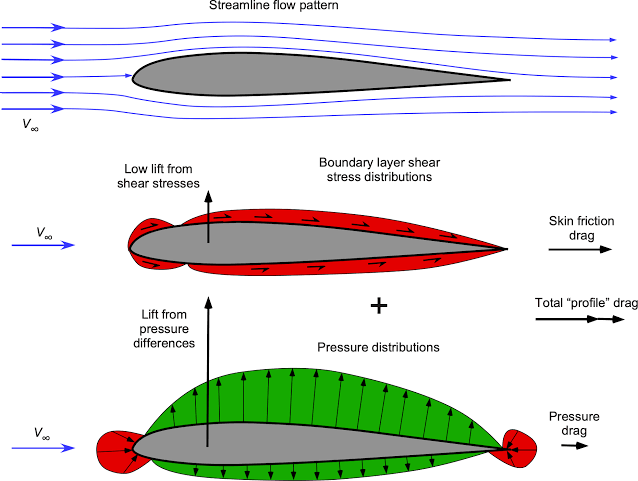
\includegraphics[width=0.5\linewidth]{Images/Chapter02/image.png}
    \caption{Aerodynamic forces on an airfoil. Source: Eagle Pubs}
    \label{fig:aerodynamic_forcex}
\end{figure}

\vspace{2ex}
As illustrated in Figure \ref{fig:aerodynamic_forcex}, the Cartesian force components $(F_x, F_y)$ are projected into the aerodynamic reference frame using the angle of attack $\alpha$:
\begin{equation}
  D = F_x\cos\alpha + F_y\sin\alpha, \qquad
  L = -F_x\sin\alpha + F_y\cos\alpha.
\end{equation}
\vspace{2ex}

The forces are normalized by the dynamic pressure $q_\infty$ and the
reference surface $S_\text{ref}$ (which corresponds to the chord length in 2D simulations):
\begin{equation}
  q_\infty = \tfrac{1}{2}\rho U_\infty^2, \qquad
  C_L = \frac{L}{q_\infty S_\text{ref}}, \qquad
  C_D = \frac{D}{q_\infty S_\text{ref}}.
\end{equation}

\paragraph{Implementation details}

This procedure is encapsuled in a header-only utility class \texttt{AerodynamicCoefficientsEvaluator} that exposes a single method:
\begin{lstlisting}[style=cppstyle, caption={Method from \texttt{AerodynamicCoefficientsEvaluator}.}]
compute_coefficients(tag, density, U_inf, S_ref, alpha)
\end{lstlisting}
It is registered as a callback via \texttt{FluidDynamics::set\_end\_timestep\_callback}, so it executes
automatically after each successful NS time step. Results are then appended to a CSV file (\texttt{force.csv}) with columns \texttt{time, F\_lift, F\_drag, C\_L, C\_D}.

% MODIFICA 3 — parametro di configurazione
\subsubsection{Configuration}

The turbulence model is selected via the parameter \texttt{"Turbulence model": "Spalart-Allmaras"} in the JSON configuration file.\\

For backward compatibility, \texttt{FluidDynamicsSA} also accepts the legacy value \texttt{"None"}, overriding it internally with \texttt{Turbulence::SpalartAllmaras} after \texttt{parse\_parameters}.\\

The \texttt{enum class Turbulence} in \texttt{fluid\_dynamics.hpp} was extended accordingly:
\begin{lstlisting}[style=cppstyle, caption={Extension of the class \texttt{Turbolence}.}]
enum class Turbulence { None, VMS_LES, SpalartAllmaras };
\end{lstlisting}

% ---------------------------------------------------------------
\subsection{Computational framework and execution workflow}

This section details the computational environment and the end-to-end workflow established for the simulation.

\subsubsection{HPC platform and software stack}

All simulations were executed on \textbf{Leonardo} at CINECA (Bologna), targeting the \texttt{dcgp\_usr\_prod} partition (Intel Sapphire Rapids nodes, 112~cores per node) under the EuroHPC allocation \texttt{EUHPC\_D35\_025}, with job submission managed by the SLURM scheduler.\\

The simulation framework is \texttt{LifeX} 2.1, introduced in Section~\ref{sec:lifex_impl}, compiled against \dealii 9.7.1 with \textbf{Trilinos} as the linear-algebra backend, MPICH 4.0 for distributed-memory parallelism, and HDF5 1.14.5 for field output in XDMF format. Meshes are generated externally with Gmsh and read by \textbf{\lifex} in MSH~2.2 format.\\

The full software stack is delivered to the compute nodes through an Apptainer image (\texttt{lifex\_env.sif}) maintained by the \textbf{\lifex} developers, which removes the need for any host-level \texttt{module load} of HPC libraries; the build procedure and the rationale behind this choice are detailed in Section~\ref{sec:container_build}.\\

The resources allocated for each run of the simulation campaign are summarized in Table~\ref{tab:hpc_resources}.

\begin{table}[H]
  \centering
  \begin{tabular}{ll}
    \hline
    \textbf{Component} & \textbf{Specification} \\
    \hline
    Cluster & Leonardo @ CINECA (EuroHPC) \\
    Partition & \texttt{dcgp\_usr\_prod} \\
    CPU & Intel Sapphire Rapids \\
    Cores per node & 112 \\
    MPI ranks per simulation & 8 \\
    Wall-time per run & up to 24~h \\
    Software stack & LifeX 2.1 / deal.II 9.7.1 / Trilinos / MPICH 4.0 / HDF5 1.14.5 \\
    Container runtime & Apptainer 1.4.5 (image \texttt{lifex\_env.sif}) \\
    \hline
  \end{tabular}
  \caption{Computational resources for the simulation campaign on Leonardo.}
  \label{tab:hpc_resources}
\end{table}


\subsubsection{Containerization and build process}
\label{sec:container_build}

The compute nodes of Leonardo do not expose a pre-configured HPC software stack through the \texttt{module} command, which only loads base system libraries. A native build of \textbf{\lifex} on the cluster would therefore require manually compiling \dealii~9.7 together with all its required backends\footnote{\texttt{Trilinos} (used by \texttt{LinearAlgebraTrilinos} and the \texttt{sacado\_dfad} AD operators), PETSc, p4est, VTK, Boost, and HDF5}, an operation that is both fragile and not portable across nodes. The entire toolchain was therefore packaged into an Apptainer image and executed through the container runtime available on the compute nodes (Apptainer~1.4.5), so that the build environment is identical to the execution environment.\\

Identifying an image that simultaneously satisfies all \textbf{\lifex} dependencies required iterating over several candidates, summarized in Table~\ref{tab:container_attempts}, encountering a series of incompatibilities:
\begin{itemize}[itemsep=2ex, topsep=2ex]
    \item[-] the Spack stack pre-installed on Leonardo provides \texttt{dealii@9.6.2}, but only with the \texttt{\textasciitilde{}trilinos} variant, which is incompatible with \textbf{\lifex}~2.1;
    \item[-] the official \texttt{dealii/dealii} Docker images expose \dealii~9.7 with all required backends, but lack the \texttt{boost\_filesystemConfig.cmake} component required by the \textbf{\lifex} CMake configuration;
    \item[-] an earlier MOX \texttt{mk} container shipping \dealii~9.5.1 fails to compile \textbf{\lifex}~2.1 due to API changes in \texttt{get\_mpi\_communicator}, \texttt{CellStatus}, and \texttt{AffineConstraints} that occurred upstream between 9.5 and 9.7
\end{itemize}
The image finally adopted, \texttt{mk-dealiimaster\_latest.sif}, is the MOX MK container with the \dealii module tracking the upstream master branch (\dealii~9.7), together with matching \texttt{vtk}, \texttt{boost}, \texttt{trilinos}, \texttt{petsc}, \texttt{p4est}, and \texttt{hdf5} modules, activated inside the container by sourcing \texttt{/u/sw/etc/profile} and loading the relevant modules.

\begin{table}[h!]
  \centering
  \footnotesize
  \begin{tabular}{p{0.27\textwidth} p{0.33\textwidth} p{0.30\textwidth}}
    \hline
    \textbf{Stack} & \textbf{Components} & \textbf{Outcome} \\
    \hline
    Spack \texttt{dealii@9.6.2} (Leonardo) &
    deal.II \texttt{\textasciitilde{}trilinos}, PETSc, MPICH &
    Missing Trilinos/Sacado required by LifeX 2.1 \\
    \texttt{dealii/dealii} Docker images (\texttt{v9.7.1-jammy}, \texttt{master-jammy}, \texttt{v9.7.1-noble}) &
    deal.II 9.7.1 with Trilinos, PETSc, p4est, VTK, HDF5 &
    \texttt{boost\_filesystemConfig.cmake} missing in the image \\
    MOX \texttt{mk} container (deal.II 9.5.1) &
    deal.II 9.5.1, Boost 1.76, VTK, HDF5 &
    API mismatch: LifeX 2.1 requires deal.II $\geq$ 9.7 \\
    \texttt{mk-dealiimaster\_latest.sif} &
    MK toolchain with deal.II master ($\geq$ 9.7), Boost, VTK, Trilinos, PETSc, p4est, HDF5 &
    \textbf{Adopted} for the simulation campaign \\
    \hline
  \end{tabular}
  \caption{Container strategies evaluated for building LifeX on Leonardo.}
  \label{tab:container_attempts}
\end{table}

\vspace{2ex}

The CMake configuration is invoked through \texttt{apptainer exec --cleanenv --bind}, which strips host environment contamination and mounts the workspace inside the container. Because the simulation campaign is purely two-dimensional, the build is configured with \texttt{-DLIFEX\_DIM=2} and restricted to the two example targets actually used, \texttt{example\_fluid\_dynamics\_airfoil} and \texttt{example\_fluid\_dynamics\_external\_flow}. A global \texttt{make all} cannot be used in 2D because some files in the test suite (e.g.\ \texttt{tests/multidomain\_laplace/laplace.cpp}) rely on overloads of \texttt{GridTools::rotate} that exist only for three-dimensional triangulations, and the resulting compilation error stops the whole build.\\
The complete build script is reported in Listing~\ref{lst:job_build}.

\begin{lstlisting}[style=bashstyle, caption={SLURM build script for LifeX on Leonardo (\texttt{job\_build\_leonardo.sh}). The Apptainer image is invoked through the legacy \texttt{singularity} command alias.}, label={lst:job_build}]
#!/bin/bash
#SBATCH -A EUHPC_D35_025
#SBATCH -p dcgp_usr_prod
#SBATCH --time=00:24:00
#SBATCH -N 1
#SBATCH --ntasks-per-node=112
#SBATCH --job-name=lifex_build

set -euo pipefail

WORK_DIR="$HOME/Ice_acceleration_model_on_airplane_wing"
SIF="${WORK_DIR}/containers/mk-dealiimaster_latest.sif"
SRC_SUBDIR="external/lifex-public"
BUILD_SUBDIR="external/lifex-public/build_2d"

rm -rf "${WORK_DIR}/${BUILD_SUBDIR}"

singularity exec --cleanenv \
  --bind "${WORK_DIR}:/work" \
  --bind /dev/shm:/dev/shm \
  "${SIF}" bash -c "
    source /u/sw/etc/profile
    module load gcc-glibc dealii vtk

    cmake -B /work/${BUILD_SUBDIR} -S /work/${SRC_SUBDIR} \
      -DCMAKE_BUILD_TYPE=Release \
      -DLIFEX_DIM=2 \
      -DDEAL_II_DIR=\${mkDealiiPrefix} \
      -DLin_ALG=Trilinos

    cmake --build /work/${BUILD_SUBDIR} \
      --target example_fluid_dynamics_airfoil \
                example_fluid_dynamics_external_flow \
      -j 112
  "
\end{lstlisting}

\subsubsection{Mesh generation and pre-processing pipeline}\label{sec:mesh}

The computational meshes are generated with Gmsh from parametric \texttt{.geo} scripts, driven by a set of Python generators (\texttt{generate\_geo*.py}, \texttt{naca\_generator\_v*.py}) that expose the airfoil profile (NACA~0006 through NACA~0018), the domain extent, and the boundary-layer structure as input parameters.\\

The resulting mesh is hybrid: a structured layer of quadrilaterals wraps the airfoil surface to resolve the boundary layer, while the outer region is filled with unstructured triangles. Boundary entities follow a fixed tagging convention (\texttt{1}~=~inlet, \texttt{2}~=~outlet, \texttt{3}~=~airfoil wall) matching the tags expected by the \textbf{\lifex} configuration (Section~\ref{sec:lifex_impl}), and the mesh is exported in the MSH~2.2 format read natively by \dealii.\\

In accordance with the wall-resolved turbulence modeling approach described in Section~\ref{sec:02_bc}, the near-wall region is carefully refined. The height of the first cell layer is adjusted until the estimated dimensionless wall distance satisfies the criterion $y^+ \lesssim 1$ at a Reynolds number of $\mathrm{Re}=10^6$. This ensures that the use of a homogeneous Dirichlet condition for $\tilde{\nu}$ is physically valid.\\

Because a single malformed mesh wastes hours of allocated CPU time, every mesh is screened by a pre-processing pipeline before submission. Four independent Python checks are run in sequence:
\begin{itemize}[itemsep=2ex, topsep=2ex]
  \item[-] \texttt{mesh\_info.py} reports the node and element counts grouped by element type and physical tag and verifies that the inlet, outlet, and airfoil tags are all present;
  \item[-] \texttt{check\_extents.py} computes the bounding box of each tagged boundary, confirming that the inlet, outlet and airfoil entities are positioned where the geometry expects them;
  \item[-] \texttt{check\_jacobians.py} reads the mesh through \texttt{meshio} and computes the signed area of every quadrilateral via the cross product of its diagonals, flagging inverted or non-convex cells that would produce a negative Jacobian;
  \item[-] \texttt{check\_yplus.py} estimates the wall-normal $y^+$ at the first node by measuring the height of the cells adjacent to the airfoil edges and applying a flat-plate skin-friction correlation ($u_\tau/U_\infty \approx 0.036$), consistent with the estimate in Section~\ref{sec:02_bc}.
\end{itemize}
Any mesh that fails one or more of these checks is automatically discarded and regenerated. An example of a mesh that has passed this quality control pipeline, used for the NACA~0012 simulations, is shown in Figure~\ref{fig:mesh}.

\begin{figure}[!htbp]
  \centering
  \subfloat[Overall domain]{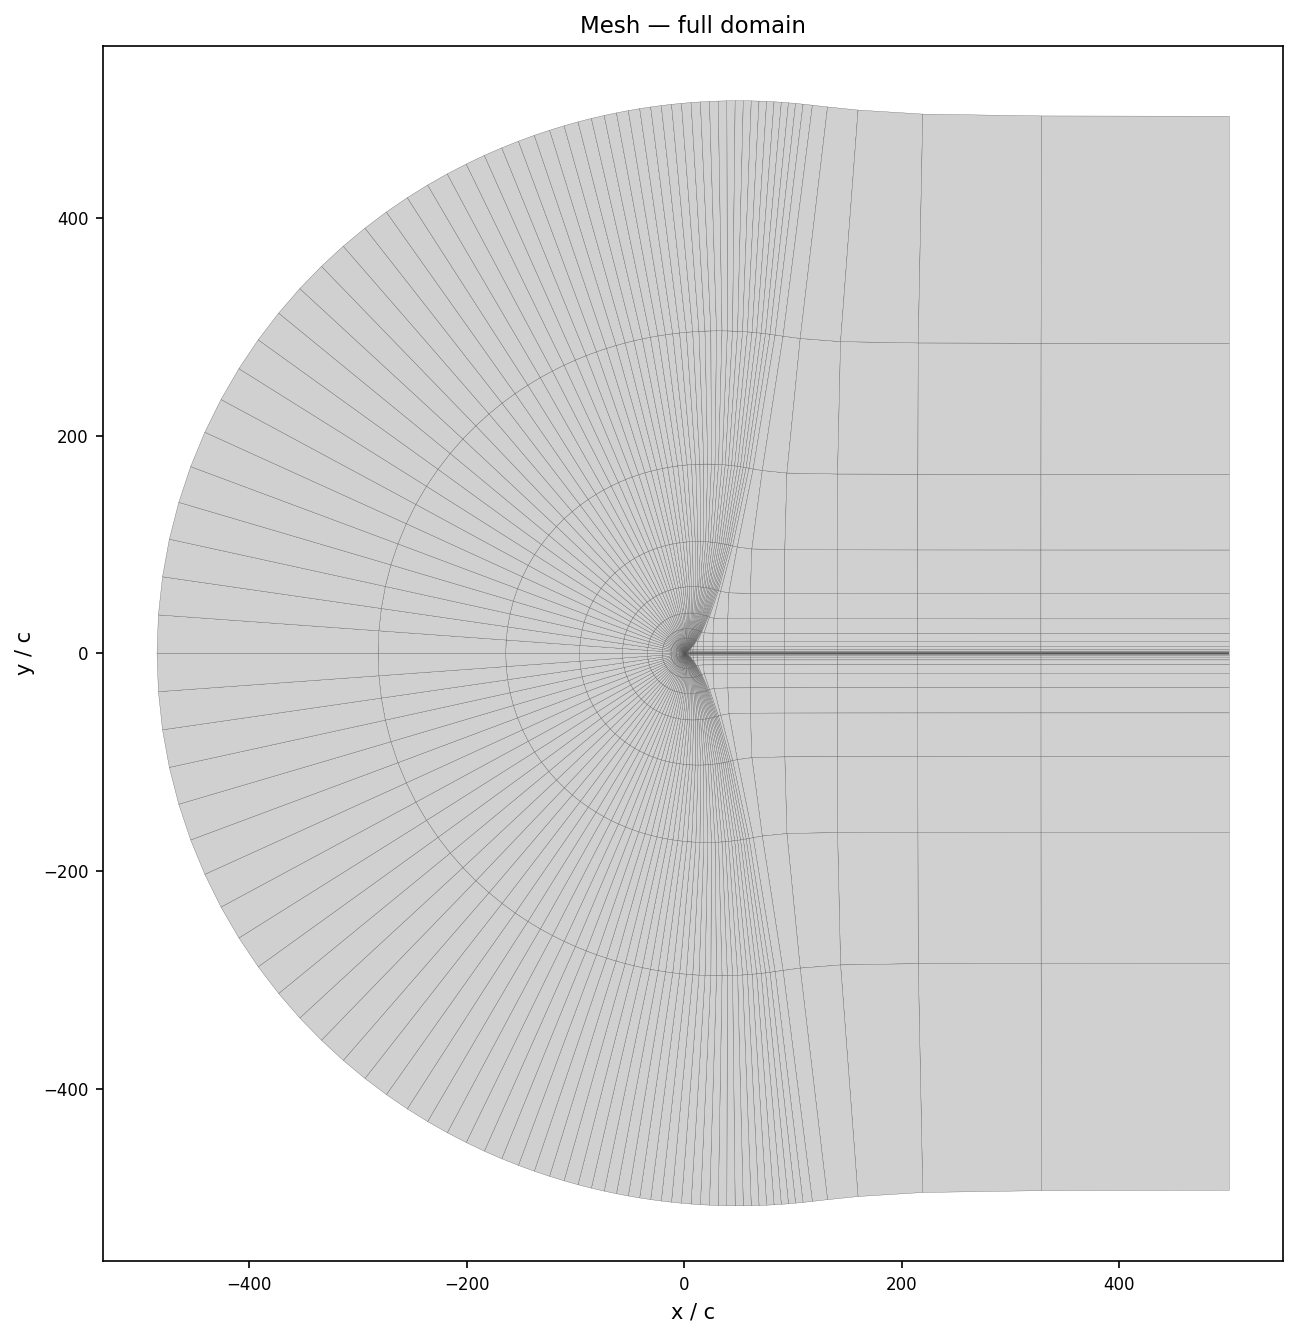
\includegraphics[width=0.45\textwidth]{Chapter02/mesh_overview.png}}
  \hfill
  \subfloat[Leading edge detail]{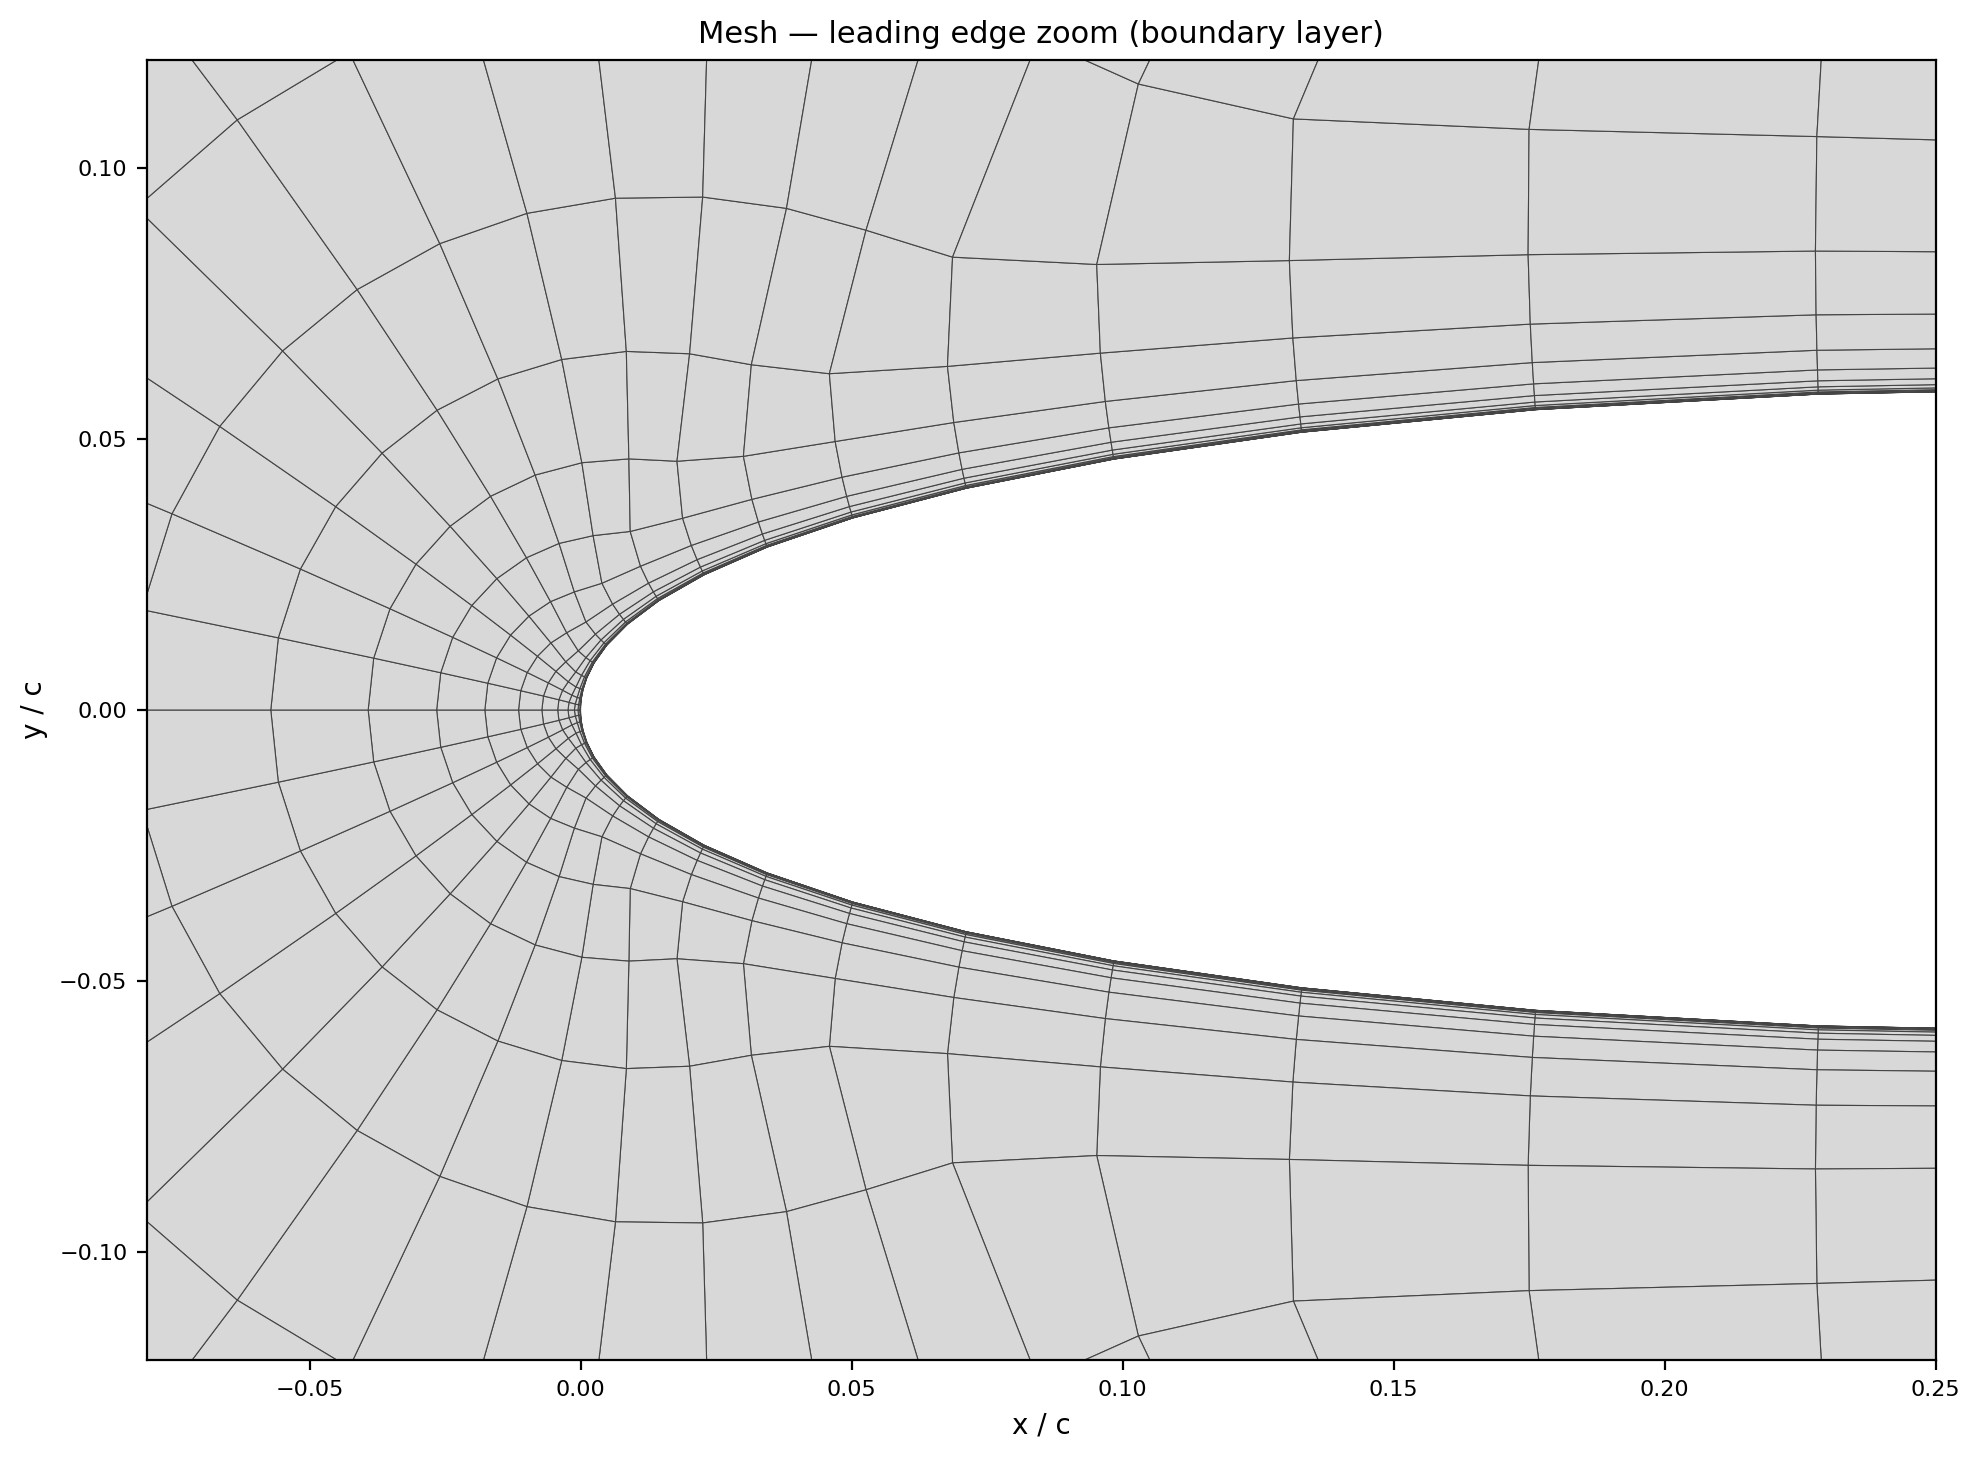
\includegraphics[width=0.45\textwidth]{Chapter02/mesh_LE_zoom.png}}
  \caption{Computational mesh for the NACA~0012 airfoil. (a) Overall domain, with a structured quadrilateral boundary layer around the profile and an unstructured triangular outer region. (b) Detail of the wall-resolved boundary layer at the leading edge, refined to give $y^+ \lesssim 1$ at $\mathrm{Re}=10^6$.}
  \label{fig:mesh}
\end{figure}

\subsubsection{Simulation execution and post-processing}
\label{sec:execution}

Each simulation is launched as a single-node SLURM job that runs the \textbf{\lifex} executable inside the Apptainer container with \texttt{mpirun -n 8}, distributing the mesh across eight MPI ranks on the \texttt{dcgp\_usr\_prod} partition.\\

The workspace is bind-mounted into the container and the run-time configuration is supplied as a JSON file, following the parameter structure described in Section~\ref{sec:lifex_impl}: the turbulence model is activated through \texttt{"Turbulence model": "Spalart-Allmaras"}, and the Reynolds number is set implicitly through the kinematic viscosity ($\nu = 10^{-6}$ with $U_\infty = 1$ and chord $c = 1$, giving $\mathrm{Re} = 10^6$). Before execution, the configuration file is copied into the run directory \texttt{output/run\_\$\{SLURM\_JOB\_ID\}/} as \texttt{config\_used.json}, so that every result remains paired with the exact parameters that produced it.\\

During the run, the solver generates two primary forms of output: a time history of the aerodynamic coefficients, which is appended to \texttt{force.csv}, and the full velocity, pressure, and turbulent-viscosity fields, saved as HDF5 files with corresponding XDMF descriptors for visualization in ParaView. The complete SLURM submission script orchestrating this process is reported in Listing~\ref{lst:job_run}.\\

\begin{lstlisting}[style=bashstyle,
  caption={SLURM run script for a single simulation (\texttt{job\_run\_leonardo.sh}).},
  label={lst:job_run}]
#!/bin/bash
#SBATCH -A EUHPC_D35_025
#SBATCH -p dcgp_usr_prod
#SBATCH --time=24:00:00
#SBATCH -N 1
#SBATCH --ntasks-per-node=8
#SBATCH --job-name=lifex_run
#SBATCH -o output/run_%j/solver.log

set -euo pipefail

WORK_DIR="$HOME/Ice_acceleration_model_on_airplane_wing"
SIF="${WORK_DIR}/containers/mk-dealiimaster_latest.sif"
EXEC="/work/external/lifex-public/build_2d/examples/fluid_dynamics_airfoil
      /lifex_example_fluid_dynamics_airfoil"
CONFIG="/work/cases/naca0012/config_new_method.json"
RUN_DIR="${WORK_DIR}/output/run_${SLURM_JOB_ID}"

mkdir -p "${RUN_DIR}"
cp "${WORK_DIR}/cases/naca0012/config_new_method.json" "${RUN_DIR}/config_used.json"

singularity exec --cleanenv \
  --bind "${WORK_DIR}:/work" \
  --bind /dev/shm:/dev/shm \
  "${SIF}" bash -c "
    source /u/sw/etc/profile
    module load gcc-glibc dealii vtk
    export LD_LIBRARY_PATH=/work/external/lifex-public/build_2d/lib:\$LD_LIBRARY_PATH

    cd /work/output/run_${SLURM_JOB_ID}
    mpirun -n 8 ${EXEC} ${CONFIG}
  "
\end{lstlisting}

The field output is inspected in ParaView, while the coefficient time histories are plotted with the \texttt{plot\_forces.py} script (matplotlib with the \texttt{Agg} backend, so that figures are rendered without a display on the compute nodes).\\

Figures~\ref{fig:cp} and \ref{fig:vorticity} show representative output for the NACA~0012 at $\alpha = 4^\circ$ and $\mathrm{Re} = 10^6$. The pressure coefficient field (Figure~\ref{fig:cp}) exhibits the suction peak on the upper surface near the leading edge that generates the net lift; the velocity field (Figure~\ref{fig:velocity}) shows the flow accelerating over the suction side and the thin viscous wake downstream of the trailing edge; the spanwise vorticity (Figure~\ref{fig:vorticity}) isolates the shed boundary layers in the wake.

\begin{figure}[!htbp]
  \centering
  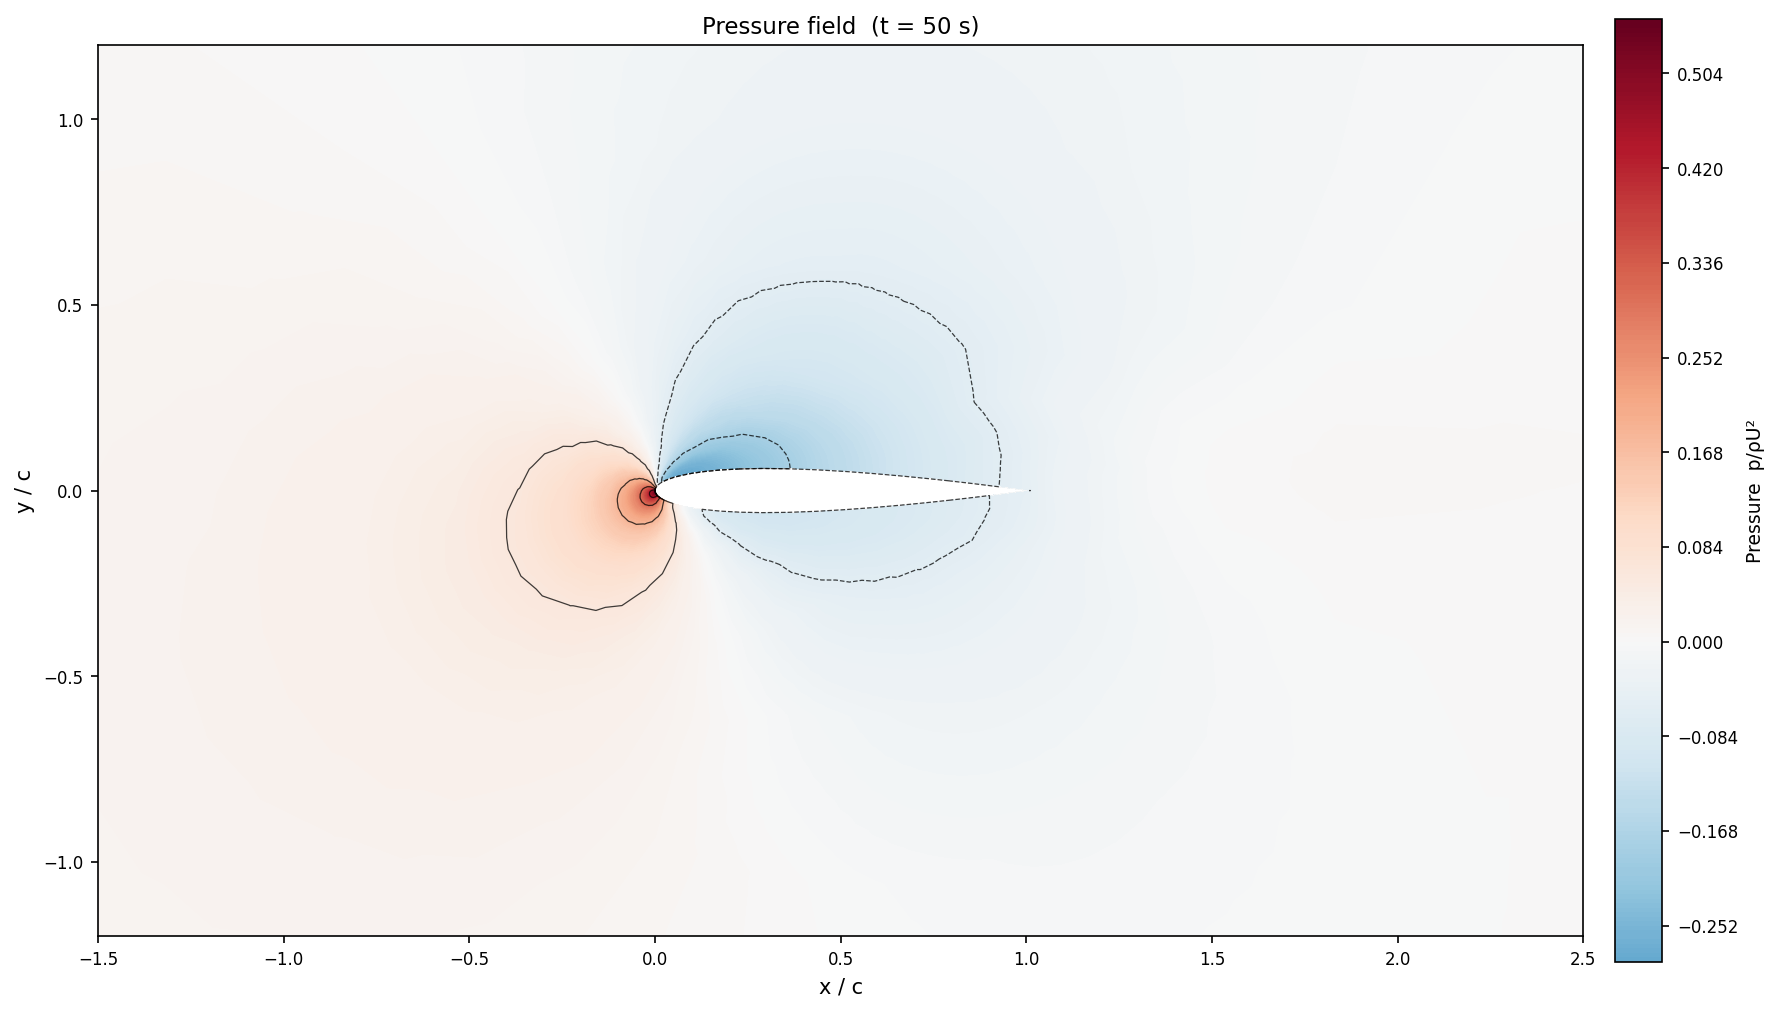
\includegraphics[width=0.65\textwidth]{Chapter02/Cp_field.png}
  \caption{Pressure coefficient field around the NACA~0012 at $\alpha = 4^\circ$, $\mathrm{Re} = 10^6$. The suction peak on the upper surface near the leading edge and the stagnation region on the lower side generate the net lift.}
  \label{fig:cp}
\end{figure}

\begin{figure}[!htbp]
  \centering
  \subfloat[Velocity magnitude with superimposed streamlines.]
    {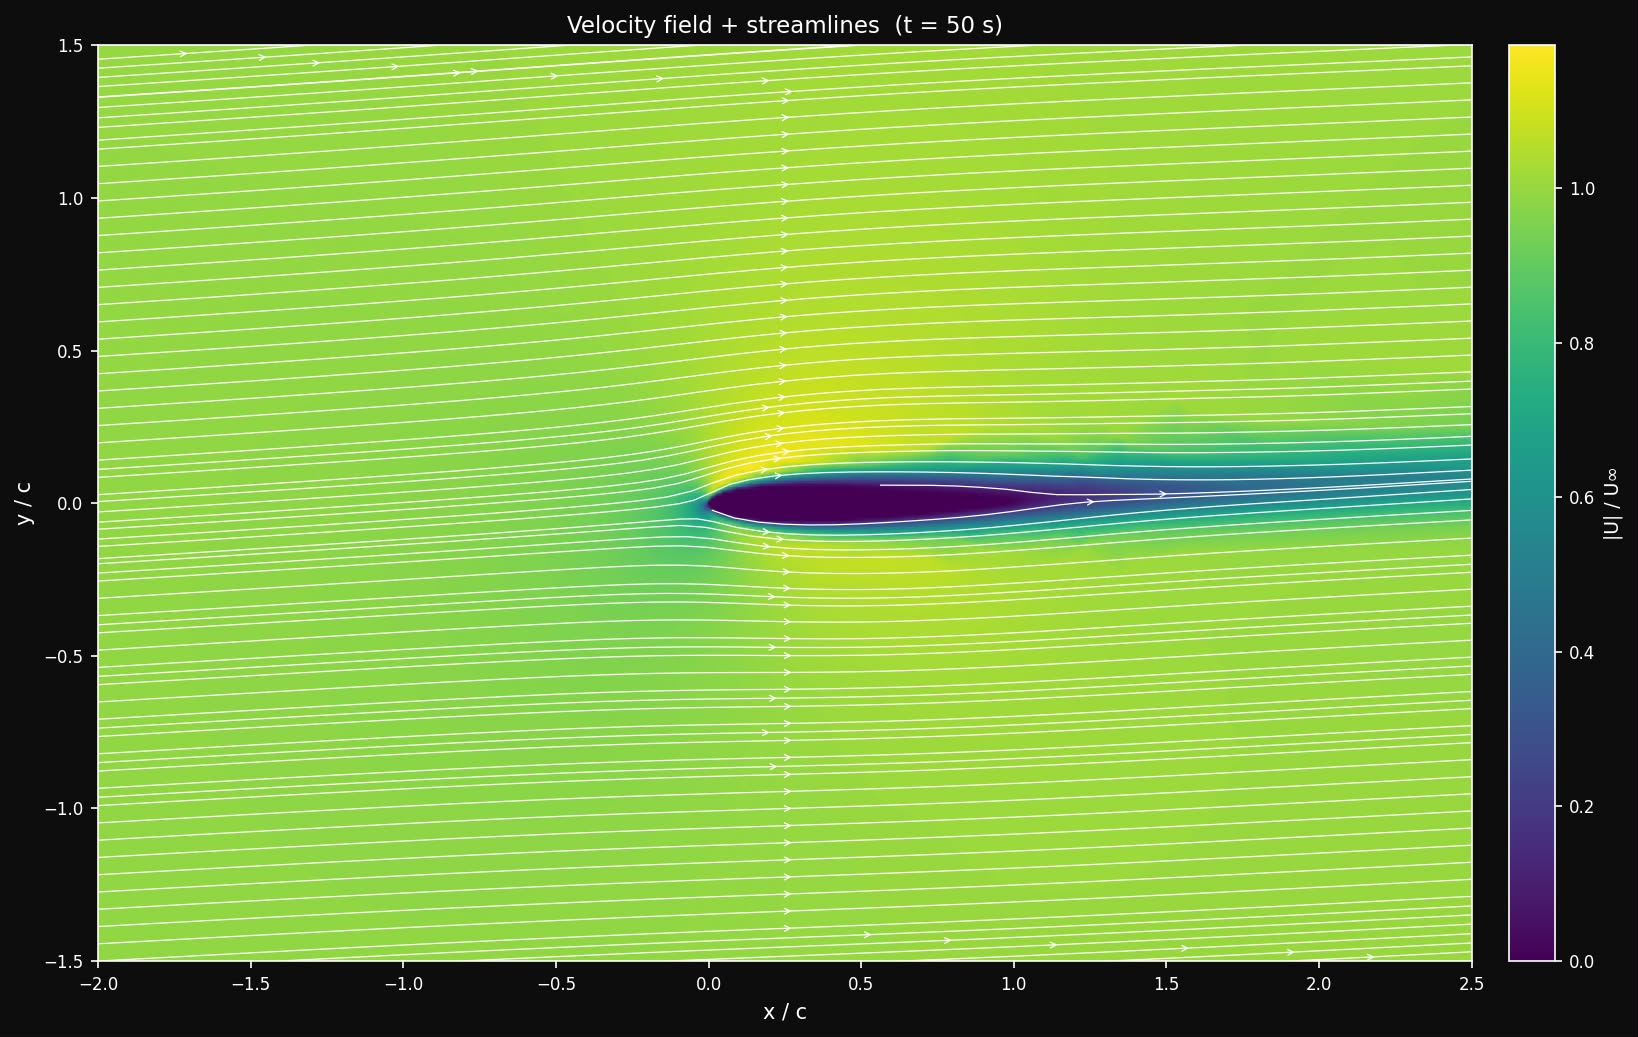
\includegraphics[width=0.45\textwidth]{Images/Chapter02/velocity_streamlines.jpeg}\label{fig:velocity}}
  \hfill
  \subfloat[Spanwise vorticity in the wake.]
    {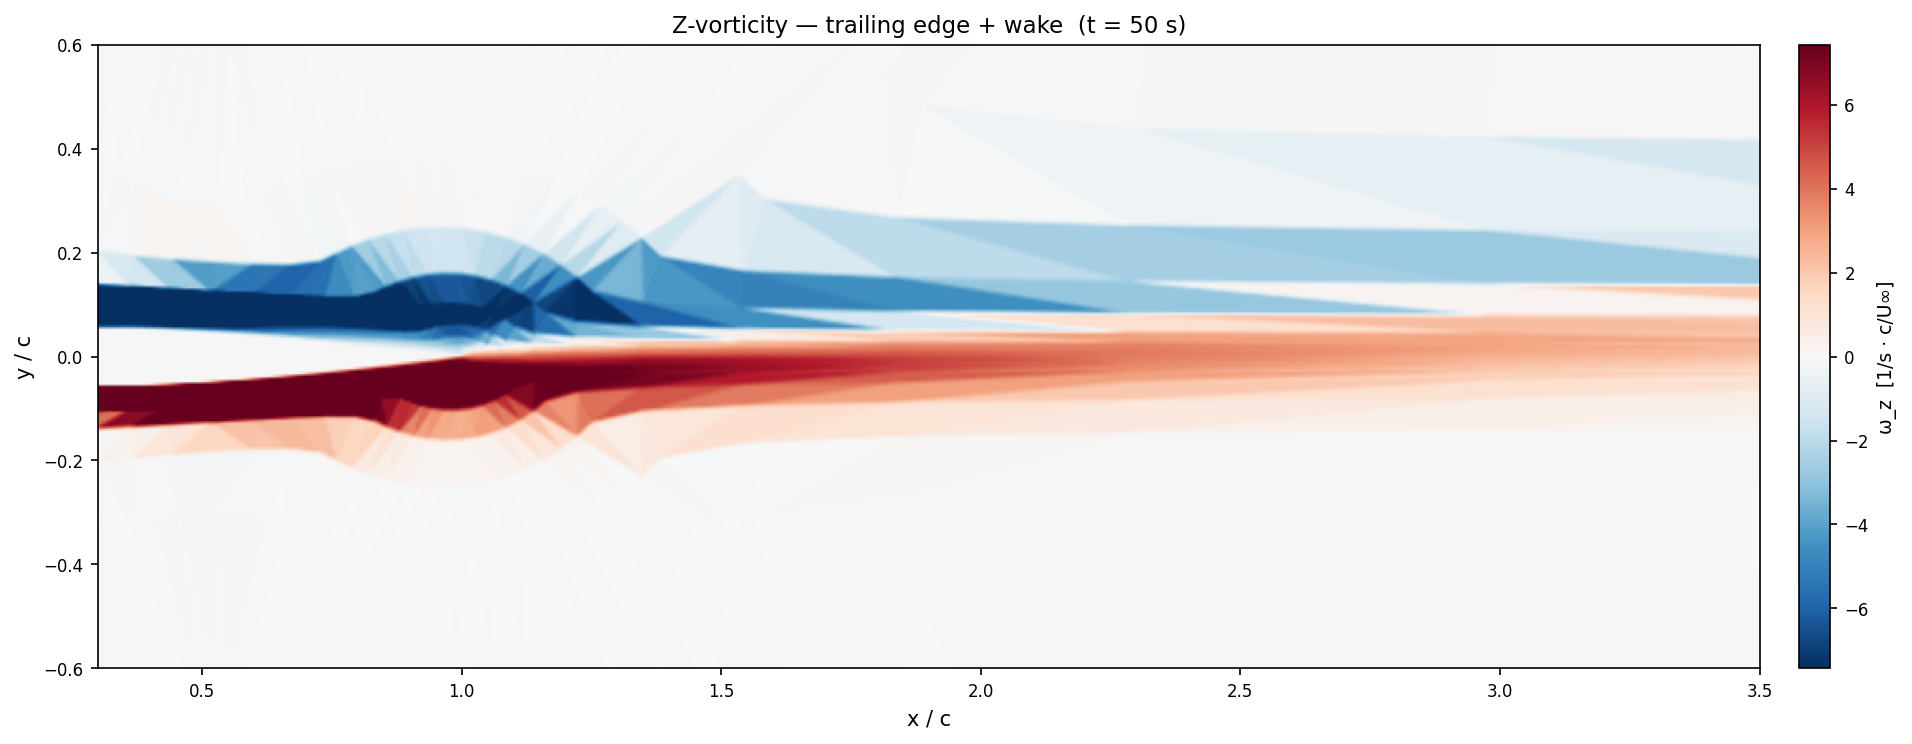
\includegraphics[width=0.45\textwidth]{Images/Chapter02/vorticity_wake.png}\label{fig:vorticity}}
  \caption{Flow field around the NACA~0012 at $\alpha = 4^\circ$, $\mathrm{Re} = 10^6$. (a) The flow accelerates over the suction side and produces a thin viscous wake downstream of the trailing edge. (b) The spanwise vorticity isolates the shed boundary layers.}
\end{figure}

\subsubsection{Dataset generation for the surrogate model}
\label{sec:dataset}

The simulation is not an end in itself: its role is to build the training set for the convolutional surrogate model presented in Section~\ref{sec:03_Convolutional_Neural_Network}.\\

To build a comprehensive dataset, the parameter space was systematically explored. For each airfoil profile in a family of symmetric NACA sections (NACA~0006 to NACA~0018), the angle of attack was swept over the range $\alpha \in \{-14^\circ, -12^\circ, \ldots, +14^\circ\}$ using templated configuration files (\texttt{config\_isa\_aoa\_*.json}).\\

For each configuration, the pipeline produces a single label: the converged lift coefficient, $C_L$. These labels populate the \texttt{Y\_cl} array of the final dataset, which is stored in the compressed NumPy format (\texttt{.npz}). The corresponding inputs are the Signed Distance Function representation of each geometry and the scalar pair of physical parameters $(\mathrm{Re}, \alpha)$.\\

Computing the lift labels with the turbulence-resolved solver, rather than with a low-fidelity panel method, is what allows the surrogate to be trained against high-fidelity data in the high-incidence regime where thin-airfoil theory no longer holds.\\ 

The same workflow extends to the iced-airfoil geometries. A modified leading edge produced by an icing model could be created in future workflows and processed through the identical execution and post-processing chain, so that the dataset can later be augmented with iced profiles without any change to the simulation pipeline. The complete workflow is summarized in Figure~\ref{fig:pipeline}.

\begin{figure}[H]
  \centering
  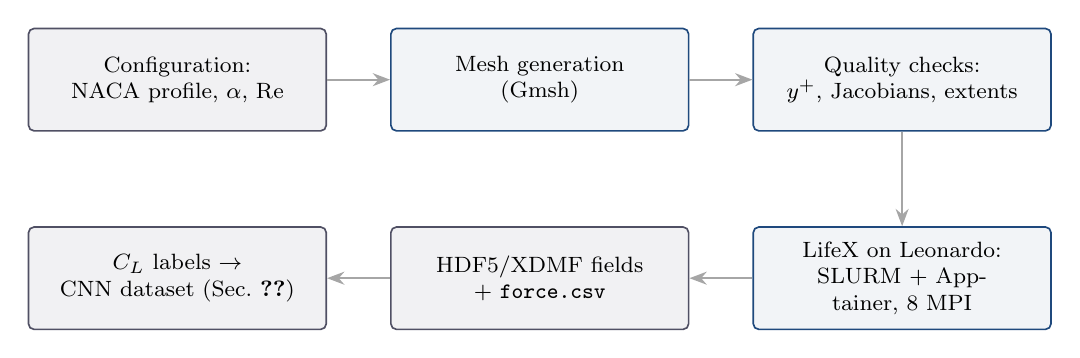
\begin{tikzpicture}[
    node distance=12mm and 8mm,
    every node/.style={font=\footnotesize},
    stage/.style={
      rectangle, rounded corners=2pt, draw=flowblue, line width=0.6pt,
      fill=flowblue!6, text width=3.5cm, align=center, inner sep=4pt,
      minimum height=13mm},
    data/.style={
      rectangle, rounded corners=2pt, draw=flowslate, line width=0.6pt,
      fill=flowslate!8, text width=3.5cm, align=center, inner sep=4pt,
      minimum height=13mm},
    arr/.style={-{Stealth[length=2.2mm]}, line width=0.7pt, draw=gray!70}
  ]

    \node[data]               (b1) {Configuration: NACA profile, $\alpha$, $\mathrm{Re}$};
    \node[stage, right=of b1] (b2) {Mesh generation\\(Gmsh)};
    \node[stage, right=of b2] (b3) {Quality checks:\\$y^+$, Jacobians, extents};
    \node[stage, below=of b3] (b4) {LifeX on Leonardo:\\SLURM + Apptainer, 8 MPI};
    \node[data,  left=of b4]  (b5) {HDF5/XDMF fields\\$+$ \texttt{force.csv}};
    \node[data,  left=of b5]  (b6) {$C_L$ labels $\rightarrow$\\CNN dataset (Sec.~\ref{sec:03_Convolutional_Neural_Network})};

    \draw[arr] (b1) -- (b2);
    \draw[arr] (b2) -- (b3);
    \draw[arr] (b3) -- (b4);
    \draw[arr] (b4) -- (b5);
    \draw[arr] (b5) -- (b6);

  \end{tikzpicture}
  \caption{End-to-end simulation pipeline (top row left to right, then bottom row right to left). Mesh generation and quality control run interactively on the login node; the solver runs as a SLURM batch job inside the Apptainer container on the compute nodes; the resulting lift coefficients feed the convolutional surrogate model of Section~\ref{sec:03_Convolutional_Neural_Network}.}
  \label{fig:pipeline}
\end{figure}
\FloatBarrier

%-----------------------------------------------------------------------------
% CAPITOLO GIULIO E ALESSIA
%-----------------------------------------------------------------------------

\section{Convolutional Neural Network}
\label{sec:03_Convolutional_Neural_Network}

Building upon the dataset established in the preceding Section \ref{sec:02_Navier-Stokes_Simulation}, this Section introduces a surrogate model designed to approximate the results of CFD simulations with a significant reduction in computational time.\\

Our approach is centered on a \textbf{Convolutional Neural Network (CNN)}, a deep learning architecture adept at learning the complex physical relationships that govern aerodynamic performance directly from simulation data. \\

Specifically, the network is designed to predict the lift coefficient ($C_L$) as a function of three key inputs: 
\begin{enumerate}
    \item the airfoil shape, represented as a \textbf{Signed Distance Function};
    \item the angle of attack ($\alpha$);
    \item the Reynolds number ($\mathrm{Re}$).
\end{enumerate}
By training on the generated simulation results, the CNN effectively learns to emulate the fluid dynamics solver, enabling near-instantaneous predictions.\\

The following sections will provide a comprehensive overview of this CNN model, from its underlying mathematical principles to its custom implementation designed for high-performance computing.

% ===================================================================
% MATHEMATICAL BACKGROUND
% ===================================================================

\subsection{Mathematical Background}

This section details the mathematical foundations of our surrogate modeling approach.\\
We first introduce the \textbf{Signed Distance Function (SDF)}, which transforms the airfoil's complex geometry into a structured grid suitable for a neural network. We then provide a comprehensive breakdown of the \textbf{Convolutional Neural Network architecture}, explaining the mathematical operations within each layer and the physics-informed training algorithm used to learn the mapping from geometry and flow conditions to the aerodynamic lift coefficient.

\subsubsection{Geometric Representation with Signed Distance Function}
\label{sec:03_SDF}

To construct a deep learning model capable of predicting aerodynamic coefficients, we need a robust method for representing the geometry of the airfoil $\Omega \subset \mathbb{R}^2$ and its boundary $\partial\Omega$ in a format suitable for Convolutional Neural Networks. Traditional boundary representations, such as coordinates of boundary points, are challenging to process with standard convolutional operators because they lack fixed spatial grids. To address this limitation, we represent the airfoil geometry using a \textbf{Signed Distance Function}, obtaining for each airfoil the result shown in Figure \ref{fig:SDF}.\\

\begin{figure}[h]
    \centering
    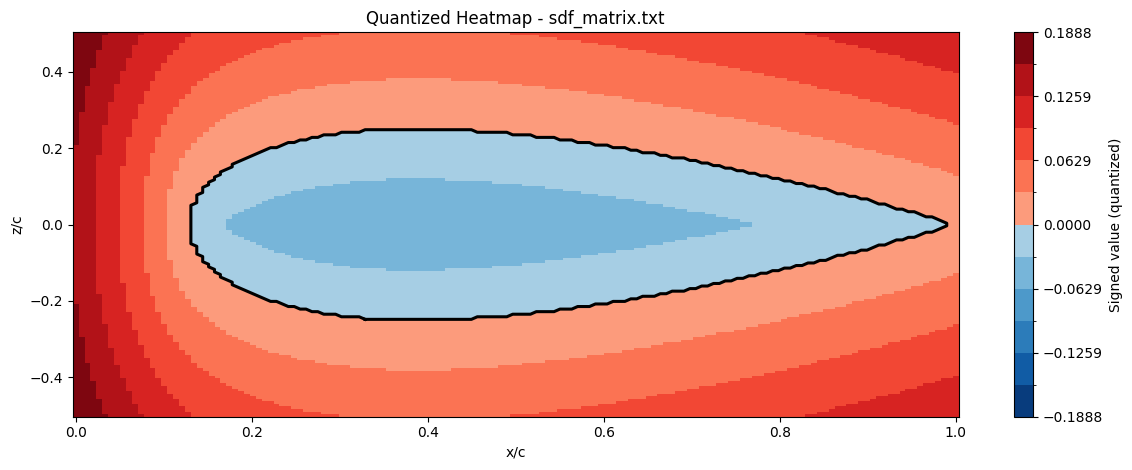
\includegraphics[width=0.65\linewidth]{Images//Chapter03/SDF.png}
    \caption{The Signed Distance Field representation of a NACA 0012 airfoil, discretized on a uniform grid. Negative values (blue) correspond to the airfoil interior, positive values (red) to the exterior while the boundary is represented by the zero-level contour (black line).}
    \label{fig:SDF}
\end{figure}

The SDF $\Phi: \mathbb{R}^2 \to \mathbb{R}$ maps any point $P = (x, z)$ in the spatial domain to its signed distance from the boundary $\partial\Omega$:
\begin{equation}
    \Phi(P) = \begin{cases}
        -d(P, \partial\Omega) & \text{if } P \in \Omega \\
        \phantom{-} d(P, \partial\Omega) & \text{if } P \notin \Omega
    \end{cases}
    \label{eq:sdf_definition}
\end{equation}
where $d(P, \partial\Omega)$ represents the Euclidean distance from the point $P$ to the boundary $\partial\Omega$:
\begin{equation}
    d(P, \partial\Omega) = \inf_{Q \in \partial\Omega} \|P - Q\|_2
    \label{eq:distance_to_boundary}
\end{equation}
Using this definition, the boundary of the airfoil is implicitly defined as the zero-level set of the function:
\begin{equation}
    \partial\Omega = \{P \in \mathbb{R}^2 \mid \Phi(P) = 0\}
\end{equation}
while the interior corresponds to negative values ($\Phi(P) < 0$) and the exterior to positive values ($\Phi(P) > 0$).\\

In our numerical implementation, the boundary $\partial\Omega$ is defined as a closed polygon composed of an ordered set of $n$ vertices $\{V_0, V_1, \dots, V_{n-1}\}$.\\
To guarantee scale invariance, the coordinates of the airfoil profile are first normalized by the chord length $c$, defined as the Euclidean distance between the leading edge point $(x_{\min}, z|_{x_{\min}})$ and the trailing edge point $(x_{\max}, z|_{x_{\max}})$:
\begin{equation}
 c = \sqrt{(x_{\max} - x_{\min})^2 + (z_{\text{at } x_{\max}} - z_{\text{at } x_{\min}})^2}
\end{equation}
where $x_{\max}$, $x_{\min}$, $z_{\max}$, and $z_{\min}$ are the extreme coordinates computed over the boundary vertices. Each vertex is then scaled by dividing its coordinates by $c$:
\begin{equation}
    V_i = \left(\frac{x_{V_i}}{c}, \frac{z_{V_i}}{c}\right)
\end{equation}
The boundary $\partial\Omega$ is then represented as the union of $n$ linear segments $S_i = [V_i, V_{i+1}]$ (with $V_n = V_0$). The minimum distance from a grid point $P$ to the boundary $\partial\Omega$ is computed by finding the minimum distance to each individual segment $S_i$:
\begin{equation}
    d(P, \partial\Omega) = \min_{i=0, \dots, n-1} d(P, S_i)
\end{equation}
For a given segment $S_i$ defined by the endpoints $A = V_i$ and $B = V_{i+1}$, any point on the infinite line passing through $A$ and $B$ can be parameterized as $P(t) = A + t(B-A)$ for $t \in \mathbb{R}$. The orthogonal projection of the point $P$ onto this line is obtained by minimizing the distance $\|P - P(t)\|^2$, which yields the projection parameter:
\begin{equation}
    t^* = \frac{(P - A) \cdot (B - A)}{\|B - A\|_2^2}
    \label{eq:03_orthogonal_projection}
\end{equation}
To restrict the projection to the finite line segment $S_i$, $t^*$ is clamped to the interval $[0, 1]$:
\begin{equation}
    t = \max\left(0, \min\left(1, t^*\right)\right)
    \label{eq:03_clamping}
\end{equation}
The projection point on the segment is then $P_{\text{proj}} = A + t(B-A)$, and the distance to the segment is:
\begin{equation}
    d(P, S_i) = \|P - P_{\text{proj}}\|_2
\end{equation}

To determine the sign of the distance field, we implement the \textbf{Winding Number Algorithm} to check whether a grid point $P$ lies inside or outside the closed boundary. The winding number $wn(P)$ computes the number of times the boundary curve wraps around the point $P$. For a closed polygon, it is computed by casting a horizontal ray starting from $P$ and pointing in the positive $x$-direction, and counting the signed crossings of this ray with the polygon edges:
\begin{itemize}
    \item[-] an \textbf{upward crossing} occurs if an edge $S_i = [V_i, V_{i+1}]$ crosses the horizontal ray from below, i.e., $V_{i, z} \le z_P < V_{i+1, z}$ and $P$ lies to the left of the directed line segment;
    \item[-] a \textbf{downward crossing} occurs if an edge $S_i$ crosses the horizontal ray from above, i.e., $V_{i+1, z} \le z_P < V_{i, z}$ and $P$ lies to the right of the directed line segment.
\end{itemize}
The relative position of the point $P$ with respect to the directed segment $[A, B]$ is determined mathematically using the 2D cross product:
\begin{equation}
    \text{cross}(P, A, B) = (A_x - x_P)(B_z - z_P) - (B_x - x_P)(A_z - z_P)
    \label{eq:cross_product}
\end{equation}
If $\text{cross}(P, A, B) > 0$, the point $P$ lies to the left of the directed segment, whereas if $\text{cross}(P, A, B) < 0$, it lies to the right. The winding number is incremented by 1 for every upward crossing and decremented by 1 for every downward crossing. A point $P$ is strictly inside the domain $\Omega$ if and only if the total winding number is non-zero:
\begin{equation}
    P \in \Omega \iff wn(P) \ne 0
\end{equation}
Once the signed distance is computed for any point, we project it onto a discrete uniform grid. The spatial domain is discretized into a Cartesian grid of size $N \times N = 150 \times 150$ over the bounding box $[X_{\min}, X_{\max}] \times [Z_{\min}, Z_{\max}]$, with:
\begin{equation}
    X_{\min} = -0.15, \quad X_{\max} = 1.01, \quad Z_{\min} = -0.12, \quad Z_{\max} = 0.12
\end{equation}
The grid spacing is defined by:
\begin{equation}
    \Delta x = \frac{X_{\max} - X_{\min}}{N-1}, \quad \Delta z = \frac{Z_{\max} - Z_{\min}}{N-1}
\end{equation}
For each grid node indexed by $(row, col)$ for $row, col = 0, \dots, N-1$, the corresponding spatial coordinates are given by:
\begin{equation}
    x_{col} = X_{\min} + col \cdot \Delta x, \quad z_{row} = Z_{\max} - row \cdot \Delta z
\end{equation}
This discretized representation yields a 2D matrix of shape $150 \times 150$, where each entry contains the signed distance value. This matrix provides a spatially structured representation of the geometry that preserves boundary details, making it perfectly suited as an input to the convolutional branch of the neural network.\\

\subsubsection{Convolutional Neural Networks for Aerodynamic Prediction}

The architecture of our \textbf{Convolutional Neural Network} is designed as a multi-input model to effectively process both the spatial geometric data and the scalar physical parameters. A high-level schematic of this design, inspired by the model presented by \cite{Cuozzo2026AIDriven}, is depicted in Figure \ref{fig:cnn_architecture}.\\

\begin{figure}[H]
    \centering
    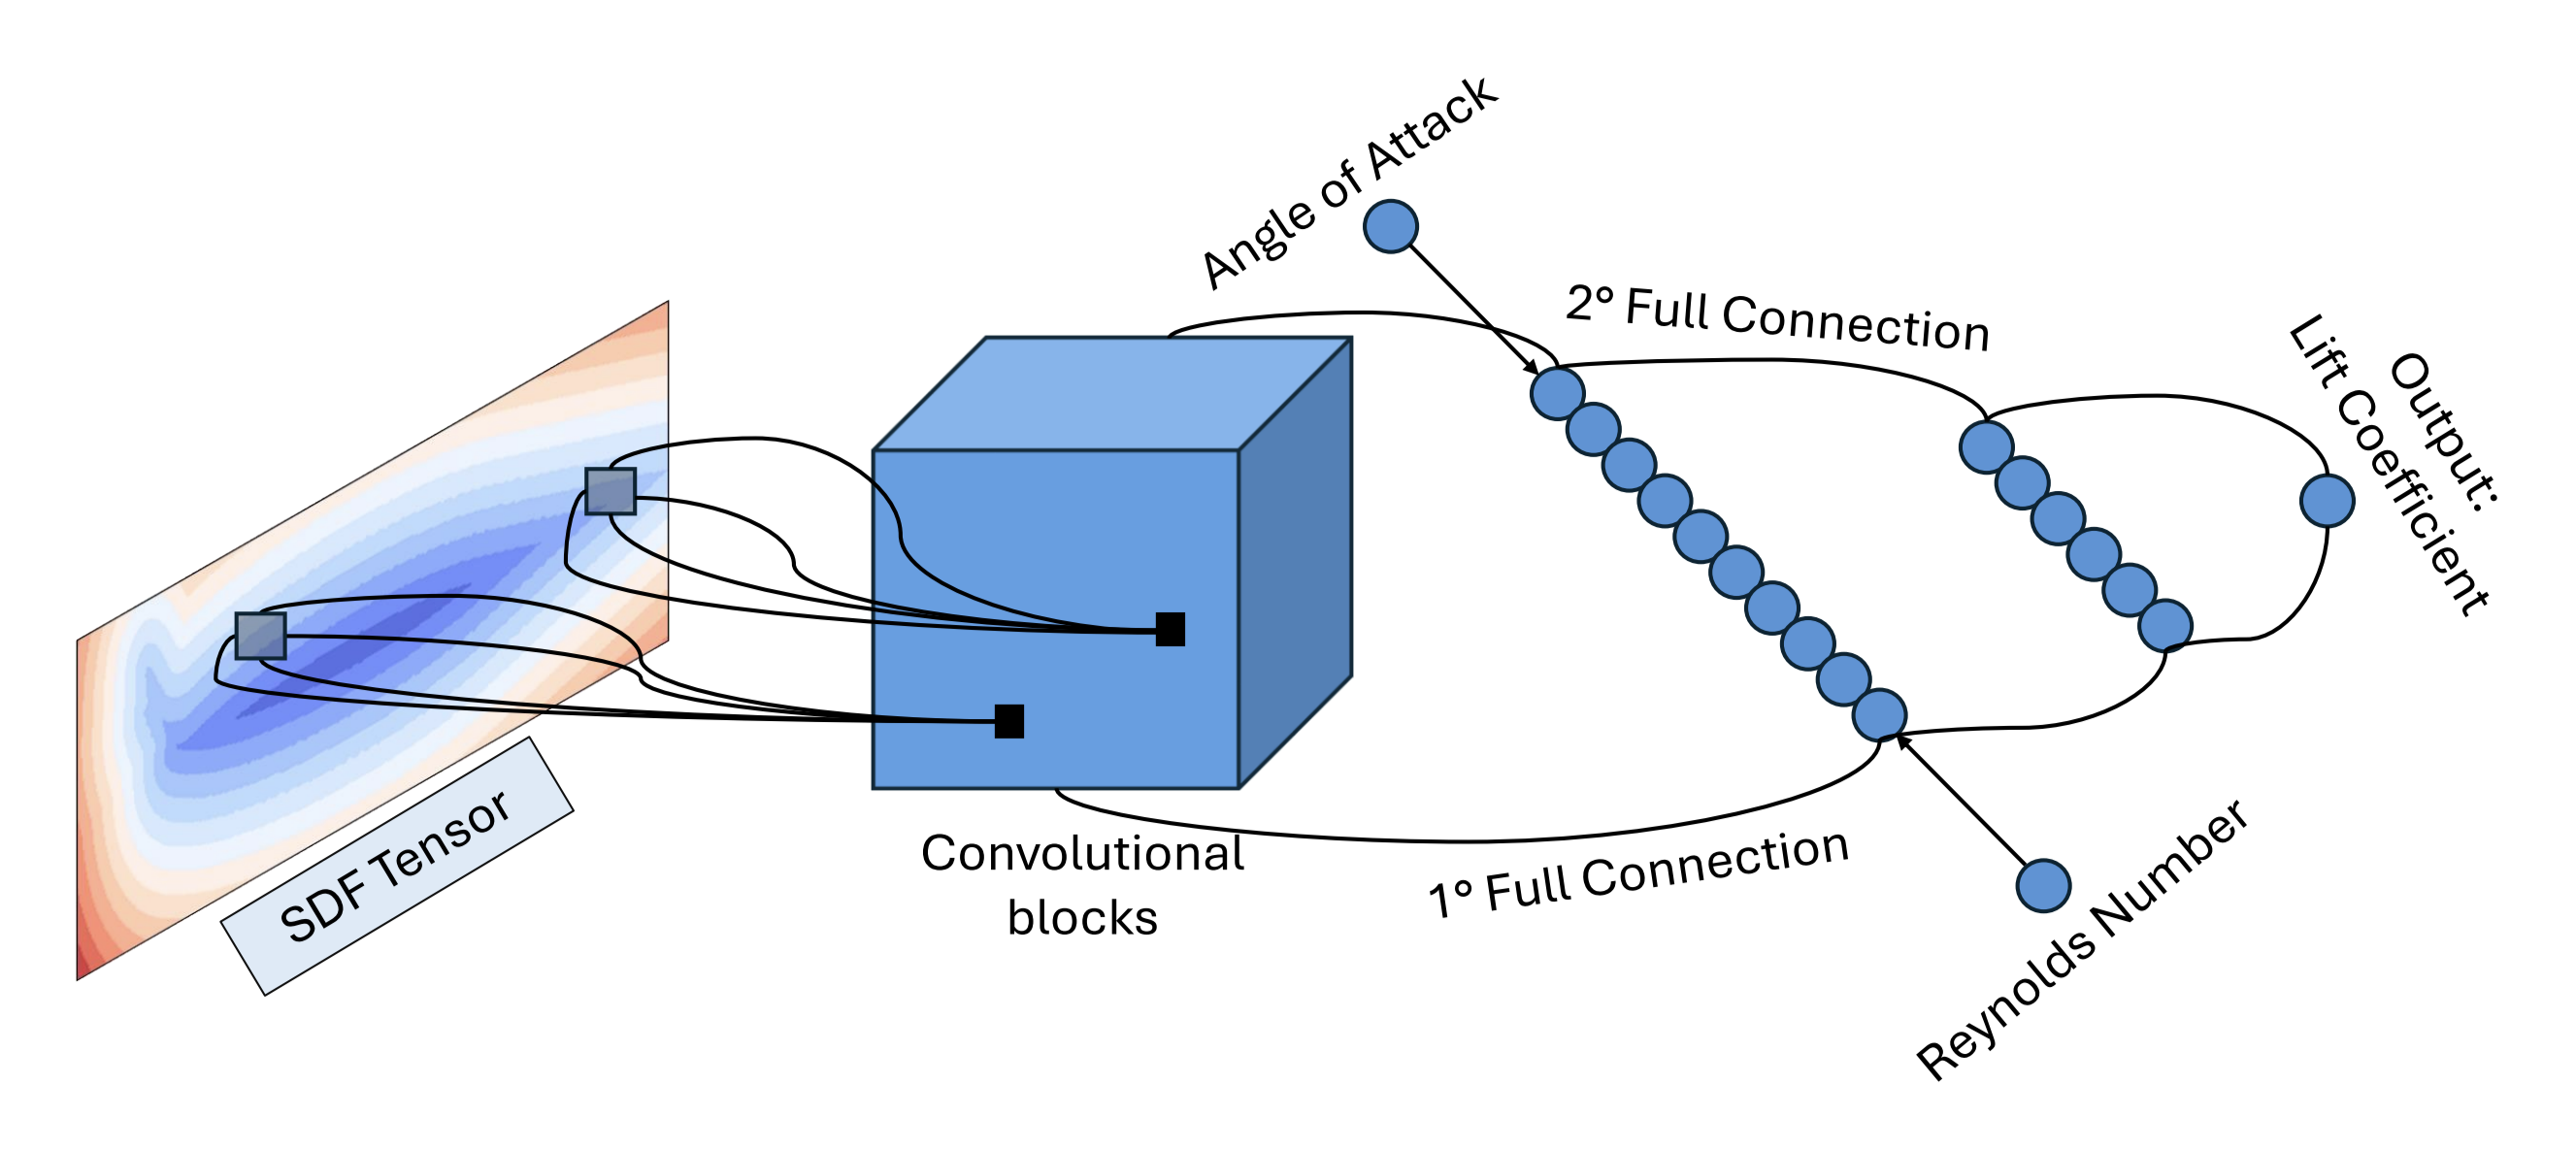
\includegraphics[width=0.8\linewidth]{Images/Chapter03/cnn_architecture.png}
    \caption{Architecture of the Convolutional Neural Network used for aerodynamic prediction.}
    \label{fig:cnn_architecture}
\end{figure}

The network is logically divided into three main components:\\ 
\begin{enumerate}[itemsep=2ex]
    \item a convolutional feature extractor, responsible for interpreting the airfoil geometry. It accepts the 2D SDF matrix as input and processes it through a series of \texttt{Conv2DLayer}s, each followed by a \texttt{LeakyReLULayer} activation. This stack of layers hierarchically extracts relevant spatial features, such as leading-edge curvature and surface details. The resulting multi-channel feature maps are then transformed into a one-dimensional vector by a \texttt{FlattenLayer}, producing a learned representation of the airfoil's shape;
    \item a feature fusion stage, in which, the flattened geometric feature vector from the convolutional branch is concatenated with the scalar physical parameters (the angle of attack and the Reynolds number) tensor using a \texttt{ConcatenateLayer}. This creates a single feature vector that contains comprehensive information about both the airfoil's shape and the current flow conditions;
    \item finally the unified vector is passed to the regression head, which consists of a sequence of \texttt{DenseLayer}s. This fully-connected network maps the combined high-level features to a single scalar output, which represents the predicted lift coefficient, $C_L$.
\end{enumerate}

\paragraph{Convolutional Layer}

The \textbf{Convolutional Layer} (\texttt{Conv2DLayer}) is an operator specifically designed to process grid-like data such as the 2D SDF. Its primary function is to detect local spatial patterns within the input by applying a set of learnable filters. The difference with the dense layer, which treats all input pixels independently, is that a convolutional layer preserves the spatial relationship between pixels by operating on localized neighborhoods.\\

At its core, the operation is a discrete 2D convolution, which can be understood as a \textit{sliding window dot product}. A small matrix of learnable weights, known as the kernel ($K$), slides over the input feature map ($I$). At each position, an element-wise multiplication between the kernel and the overlapping region of the input is performed, and the results are summed up to produce a single pixel in the output feature map ($O$).\\

For a single-channel input $I$ of size $H\times W$ and a kernel of size $F\times F$, the value of the output $O$ at position $(i,j)$ is given by:
\begin{equation}
    O(i,j)=\sum_{m=0}^{F-1}\sum_{n=0}^{F-1}I(i-m,j-n)\cdot K(m,n)+b
    \label{eq:convolutional_sum}
\end{equation}
where $b$ is a learnable scalar bias term applied to the entire output feature map.\\

The key principle here is parameter sharing: the \textit{same} kernel $K$ and bias $b$ are used across all positions of the input, allowing the network to detect the same feature regardless of where it appears in the SDF\footnote{In more details, if the kernel learns to recognize a leading edge curve of a profile, it will successfully detect the curve whether it appears at the top of the grid or in a bottom corner.}.\\

In deep networks, layers typically process multi-channel inputs. If the input feature map has $C_{in}$ channels\footnote{This is not our case, since in the SDF we have only one input channel ($C_{in}=1$).}, the kernel must be three-dimensional, with a size of $F\times F\times C_{in}$. The convolution is then performed across all channels simultaneously. The results from each channel are then summed together to produce a single value for the 2D output map.\\

To generate an output with $C_{out}$ feature maps, we simply apply $C_{out}$ independent kernels. Each kernel is responsible for learning a different spatial feature, allowing the layer to build a complete representation of the input geometry.\\

The behavior of the convolution is controlled by two hyperparameters:\\
\begin{itemize}[itemsep=2ex]
    \item[-] the stride ($S$) defines the step size the kernel matrix as it traverses the input grid. While a unit stride ($S=1$) evaluates adjacent localized neighborhoods sequentially, a stride of $S > 1$ skips spatial coordinates, downsampling the spatial resolution of the resulting feature map;
    \item[-] padding ($P$)\footnote{In our implementation, padding is set to $0$.} consists in appending a perimeter of zero-valued elements around the input grid boundaries. This can be used to control the output dimensions and mitigate the loss of information at the edges.
\end{itemize}
\vspace{2ex}
The dimensions of the output feature map ($H_{out}\times W_{out}$) are determined by the input dimensions ($H_{in}\times W_{in}$), the kernel size ($F$), the stride ($S$) and the padding ($P$) using the following formula:
\begin{equation}
    W_{out}=\frac{W_{in}-F+2P}{S}+1\quad\text{and}\quad H_{out}=\frac{H_{in}-F+2P}{S}+1
    \label{eq:03_convol}
\end{equation}
From an implementation perspective, this operation is typically realized as a set of nested loops that iterate over each position in the output map, each element of the kernel, and each input channel, performing the required multiply-accumulate operations\footnote{We will explain in a better way highlighting our \cpp implementation in Section \ref{sec:03_conv} regarding our implementation in \cpp}.

\paragraph{Non-Linear Activation (Leaky ReLU)}

After each \texttt{Conv2DLayer} or \texttt{DenseLayer} performs its linear operation, an activation function applies a non-linear transformation element-wise to its output. Without this, a deep neural network, regardless of its number of layers, would behave as a single, large linear model. The introduction of non-linearity is what gives the network its power to approximate arbitrarily complex, non-linear relationships, such as the one between airfoil geometry and lift coefficient.\\

In this project, a \textbf{Leaky Rectified Linear Unit} (Leaky ReLU) is implemented as the \texttt{LeakyReLULayer}. This function, shown in Figure \ref{fig:03_relu}, is a popular and effective choice in modern deep learning due to its computational efficiency and its ability to mitigate some of the common problems encountered during training.\\

\begin{figure}[h!]
    \centering
    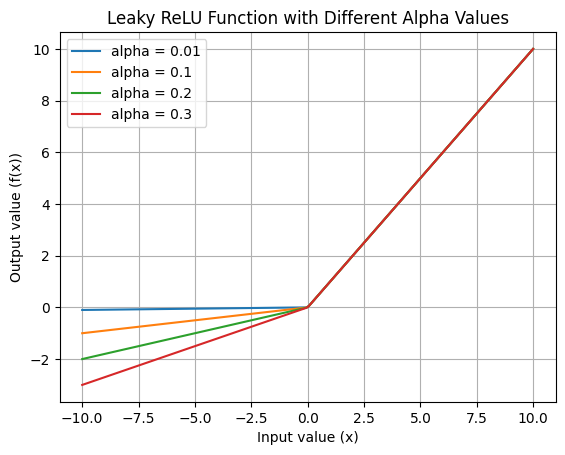
\includegraphics[width=0.4\linewidth]{Images/Chapter03/relu.png}
    \caption{Example of Leaky ReLU function with different $\alpha$.}
    \label{fig:03_relu}
\end{figure}

The Leaky ReLU function is defined mathematically as:
\begin{equation}
    \text{LeakyReLU(x)}=\begin{cases}
        x & \text{ if } x>0\\
        \alpha x&\text{ if } x\le 0
    \end{cases}
    \label{eq:03_leaky_relu}
\end{equation}
where $\alpha$ is a small, positive constant (a hyperparameter, typically set to a value like $0.01$).\\

The function behaves as a simple identity for all positive input values. For negative input values, instead of mapping them to zero like the standard ReLU function, it allows a small, non-zero gradient to pass through.\\

The primary advantage of the Leaky ReLU over the standard ReLU is its handling of negative inputs. In a standard ReLU, if a neuron's input is consistently negative, its gradient will always be zero. This means the neuron's weights will never be updated, and it can effectively "die", ceasing to contribute to the network's learning process. The Leaky ReLU prevents this "dying ReLU" problem by ensuring that a small gradient always exists, even for negative inputs.\\

From the backpropagation algorithm, the gradient of the Leaky ReLU is simple and computationally inexpensive to calculate:
\begin{equation}
    \frac{d}{dx}\text{LeakyReLU(x)}=\begin{cases}
        1 & \text{ if } x>0\\
        \alpha &\text{ if } x\le 0
    \end{cases}
    \label{eq:03_derivative_leaky_relu}
\end{equation}

During the backward pass of training, this straightforward derivative is used to scale the incoming gradient from the subsequent layer:
\begin{itemize}
    \item[-] if the input to the activation function was positive during the forward pass, the gradient passes through unchanged;
    \item[-] if it was negative, the gradient is scaled down by the factor $\alpha$.
\end{itemize}
This simple conditional check makes the backward pass for the \texttt{LeakyReLULayer} extremely fast, contributing to the overall efficiency of the training process.

\paragraph{Structural Layers}
\label{sec:03_struct_layer}

After the convolutional network has extracted a hierarchy of spatial features, the resulting multi-channel feature maps must be prepared for integration with the scalar parameters and for final processing by the regression head. This preparation is handled by two complementary \textbf{structural layers}, the \texttt{FlattenLayer} and the \texttt{ConcatenateLayer}, that are parameter-free: they do not contain any learnable weights or biases since their sole purpose is to rearrange data tensors.\\

\textbf{Flatten Layer}\\

The \texttt{FlattenLayer} links the convolutional layers and the fully-connected layers. Convolutional layers output a 4D tensor with a shape of \texttt{[Batch Size, Channels, Height, Width]}, preserving spatial information. However, dense layers require their input to be a 2D tensor of shape \texttt{[Batch Size, Features]}, where each row is a one-dimensional vector representing a single sample.\\

The flatten operation reshapes an input tensor $T_{in}$ with dimensions $[B\times C_{out}\times H_{out}\times W_{out}]$ into an output tensor $T_{out}$ with dimensions $[B\times D]$, where the new feature dimension $D$ is the product of the input's channel, height and width dimensions:
\begin{equation}
    D=C_{out}\times H_{out}\times W_{out}
\end{equation}
During the forward pass, this is a straightforward memory rearrangement.\\
During  the backward pass for backpropagation, the \texttt{FlattenLayer} performs the inverse operation: it receives an incoming gradient tensor of shape $[B\times D]$ and reshapes it back to the original 4D shape $[B\times C_{out}\times H_{out}\times W_{out}]$. This ensures that the gradients are correctly propagated back to the preceding convolutional layer in the required spatial format.\\

\textbf{Concatenate Layer}\\

Once the geometric features have been flattened into a vector, they must be combined with the scalar physical parameters by the \texttt{ConcatenateLayer}, that takes multiple input tensors and joins them together along a specified axis\footnote{In our case, this is the feature axis (axis 1)}.\\

Mathematically, given the flattened geometric feature tensor $T_{flat}$ of shape $[B\times D_1]$ and the scalar input tensor $T_{scalar}$ (containing angle of attack and Reynolds number) of shape $[B\times D_2]$, the Concatenate Layer produces an output tensor $T_{concat}$ of shape $[B\times (D_1+D_2)]$. This operation creates a unified feature vector that encodes both geometric and physical information for the network to make a prediction.\\

During backpropagation, the process is reversed. The incoming gradient tensor is split according to the original input sizes:
\begin{itemize}
    \item[-] the first $D_1$ elements of the gradient vector are passed back to the \texttt{FlattenLayer}'s branch;
    \item[-] the $D_2$ elements corresponding to the scalar inputs are also computed, although they terminate at the input layer.
\end{itemize}
\vspace{2ex}
After this fusion step, the resulting unified tensor is ready to be processed by the final regression head of the network.

\paragraph{Dense Layer and final regression}
\label{sec:03_dense_layer}

The final computational stage of the network is handled by the\textbf{ Dense Layer} (\texttt{DenseLayer}), known as a fully-connected layer. Its role is to learn the final mapping from the feature space to the target scalar value (the lift coefficient $C_L$).\\

A dense layer applies a linear transformation to its input vector. For an input vector $\mathbf x\in \mathbb R^{D_{in}}$, the layer computes an output vector $\mathbf y\in \mathbb R^{D_{out}}$ using a learnable weight matrix $W\in \mathbb R^{D_{out}\times D_{in}}$ and a learnable bias vector $\mathbf b\in\mathbb R^{D_{out}}$. The operation is defined as:
\begin{equation}
    \mathbf y=W\mathbf x+\mathbf b
\end{equation}
This operation performs a weighted sum of all input features to compute each output feature. Every neuron in the input layer is connected to every neuron in the output layer, allowing the network to model complex interactions between all elements of the input feature vector.\\

This layer is used in the regression head, which consists of a sequence of \texttt{DenseLayer}s, each followed by a \texttt{LeakyReLULayer} activation:
\begin{itemize}
    \item[-] the initial dense layers take concatenated feature vector as input. Their purpose is to find and amplify the non-linear correlations between the learned geometric features from the SDF and the raw physical parameters ($\alpha$ and $\mathrm{Re}$);
    \item[-] the last layer is configured to have a single output neuron ($D_{out}=1$) and does not have a subsequent activation function. This single neuron's output directly corresponds to the network's prediction for the lift coefficient ($C_L$).
\end{itemize}
\vspace{2ex}
During the backward pass, the dense layer must compute three distinct gradients based on the incoming gradient from the subsequent layer $\frac{\partial L}{\partial \mathbf y}$, where $L$ is the loss:
\begin{itemize}
    \item[-] the gradient with respect to the weights ($W$) is calculated as the outer product of the incoming gradient and the layer's input vector from the forward pass:
    \begin{equation}
        \frac{\partial L}{\partial W}=\frac{\partial L}{\partial \mathbf y}\cdot \underbrace{\mathbf{x^T}}_{\frac{\partial\mathbf{y}}{\partial\mathbf{W}}}
    \end{equation}
    \item[-] the gradient with respect to the biases ($b$) is equal to the incoming gradient:
    \begin{equation}
        \frac{\partial L}{\partial \mathbf b}=\frac{\partial L}{\partial \mathbf y}
    \end{equation}
    \item[-] the gradient with respect to the input ($x$) must be passed back to the preceding layer. It is computed by multiplying the transposed weight matrix by the incoming gradient:
    \begin{equation}
        \frac{\partial L}{\partial \mathbf x}=W^T\cdot\frac{\partial L}{\partial \mathbf y}
    \end{equation}
\end{itemize}
These calculations are the fundamental operations that enable the network's regression head to learn from the training data.

\paragraph{Network Training}
\label{sec:03_loss}

The process of training the neural network involves iteratively adjusting its parameters to minimize a loss function, which quantifies the discrepancy between the model's predictions and the desired outcomes. Our approach embeds physical knowledge directly into the training process, making our model a type of \textbf{Physics-Informed Neural Network (PINN)}. This is achieved through a composite loss function that balances empirical data accuracy with a theoretical physical constraint.\\

The total loss, $L$, is a weighted sum of data-driven term and a physics-informed term:
\begin{equation}
    L=L_{\text{data}}+\lambda L_{\text{physics}}
\end{equation}
where $\lambda$ is a hyperparameter that controls the strength of the physical regularization.\\

The first component is the standard \textbf{Mean Squared Error} (MSE), which measures the difference between the network's predicted lift coefficients ($P_i$) and the ground-truth values from the CFD simulations ($T_i$):
\begin{equation}
    L_{\text{data}}=\frac 1N\sum_{i=1}^N\left(P_i-T_i\right)^2
\end{equation}
This term ensures the network learns to faithfully replicate the high-fidelity simulation data generated for this work.\\

The second component acts as a physical constraint, guiding the network's predictions to be consistent with established aerodynamic theory. This term is based on \textbf{Thin-Airfoil Theory}, which provides an analytical approximation for the lift coefficient at small angles of attack. The general form of this relationship is $C_L=2\pi(\alpha-\alpha_{L=0})$, where $\alpha_{L=0}$ is the zero-lift angle of attack.\\

For symmetric airfoils, such as those in our dataset, the zero-lift angle of attack is, by definition, $\alpha_{L=0}=0$. This simplifies the theoretical relationship to the linear form:
\begin{equation}
    C_L\approx 2\pi \alpha
\end{equation}
The physical loss in the network leverages this simplified form, penalizing deviations from this theoretical relationship:
\begin{equation}
    L_{\text{physics}}=\frac 1N\sum_{i=1}^NM_i\cdot (P_i-2\pi\alpha_i)^2
\end{equation}
where $M_i$ is a mask function, introduced because Thin-Airfoil Theory is only valid in the linear flight regime. Therefore, the mask is defined as:
\begin{equation}
    M_i=\begin{cases}
        1&\text{if }|\alpha_i|\le10^\circ\\
        0&\text{if }|\alpha_i|>10^\circ
    \end{cases}
    \label{eq:03_mask}
\end{equation}
This ensures the physical constraint is only active at low angles of attack.\\
In the non-linear, high-angle-of-attack regime, the mask deactivates this term ($M_i=0$), forcing the network to rely entirely on the empirical CFD data, which accurately captures the complex flow separation phenomena.\\

By explicitly building in the assumption of symmetry, this physics-informed regularizer provides a robust theoretical anchor for the network's predictions without being applied in regimes where its underlying assumptions would be violated.

\paragraph{Optimization with Adam}
\label{sec:03_adam}

Once the backpropagation algorithm has computed the gradient of the loss function with respect to every trainable parameter in the network ($\nabla L(\theta)$, where $\theta$ represents all weights and biases), the final step in the learning process is to update these parameters. This is done using the \textbf{Adam (Adaptive Moment Estimation)} optimizer, which guides the parameters toward a minimum in the loss landscape.\\

Adam combines the advantages of the \textbf{RMSprop} and \textbf{Momentum} optimization methods. It maintains an exponentially decaying moving average of both the past gradients (first moment, the momentum term) and the past squared gradients (second moment, the adaptive learning rate term).\\

Let $g_t=\nabla L(\theta_{t-1})$ be the gradient at timestep $t$. The optimizer updates two moving averages:
\begin{itemize}
    \item[-] first moment (momentum):
    \begin{equation}
        m_t=\beta_1m_{t-1}+(1-\beta_1)g_t
    \end{equation}
    \item[-] second moment (adaptive learning rate):
    \begin{equation}
        v_t=\beta_2v_{t-1}+(1-\beta_2)g_t^2
    \end{equation}
\end{itemize}
where $\beta_1$ and $\beta_2$ are hyperparameters (typically close to 1, e.g., 0.9 and 0.999 respectively).\\

These raw moment estimates are then bias-corrected to account for their initialization at zero:
\begin{equation}
    \hat m_t=\frac{m_t}{1-\beta_1^t}\quad\text{and}\quad \hat v_t=\frac{v_t}{1-\beta_2^t}
\end{equation}
\vspace{2ex}
Finally, the parameters are updated using these corrected estimates. The update rule for a parameter $\theta$ is:
\begin{equation}
    \theta_t=\theta_{t-1}-\eta \frac{\hat m_t}{\sqrt{\hat v_t}+\varepsilon}
\end{equation}
where $\eta$ is the learning rate and $\varepsilon$ is a small constant (e.g., $10^{-8}$) to prevent division by zero.\\

The key intuition is that the update step is scaled by both a running average of the gradients (providing momentum to navigate flat regions) and an adaptive, per-parameter learning rate (scaling down updates for frequently changing parameters and scaling up updates for sparse ones). This adaptive nature makes Adam robust and generally leads to faster convergence compared to standard stochastic gradient descent.

% ===================================================================
% CODE IMPELMENTATION
% ===================================================================

\subsection{Code Implementation}

We implemented our CNN and SDF generator using an \textbf{object-oriented paradigm}. Figure \ref{fig:03_cnn_uml} provides a comprehensive \textbf{UML class diagram} detailing the structural layout, member attributes and method signatures of the system.

\begin{figure}[h!]
    \centering
    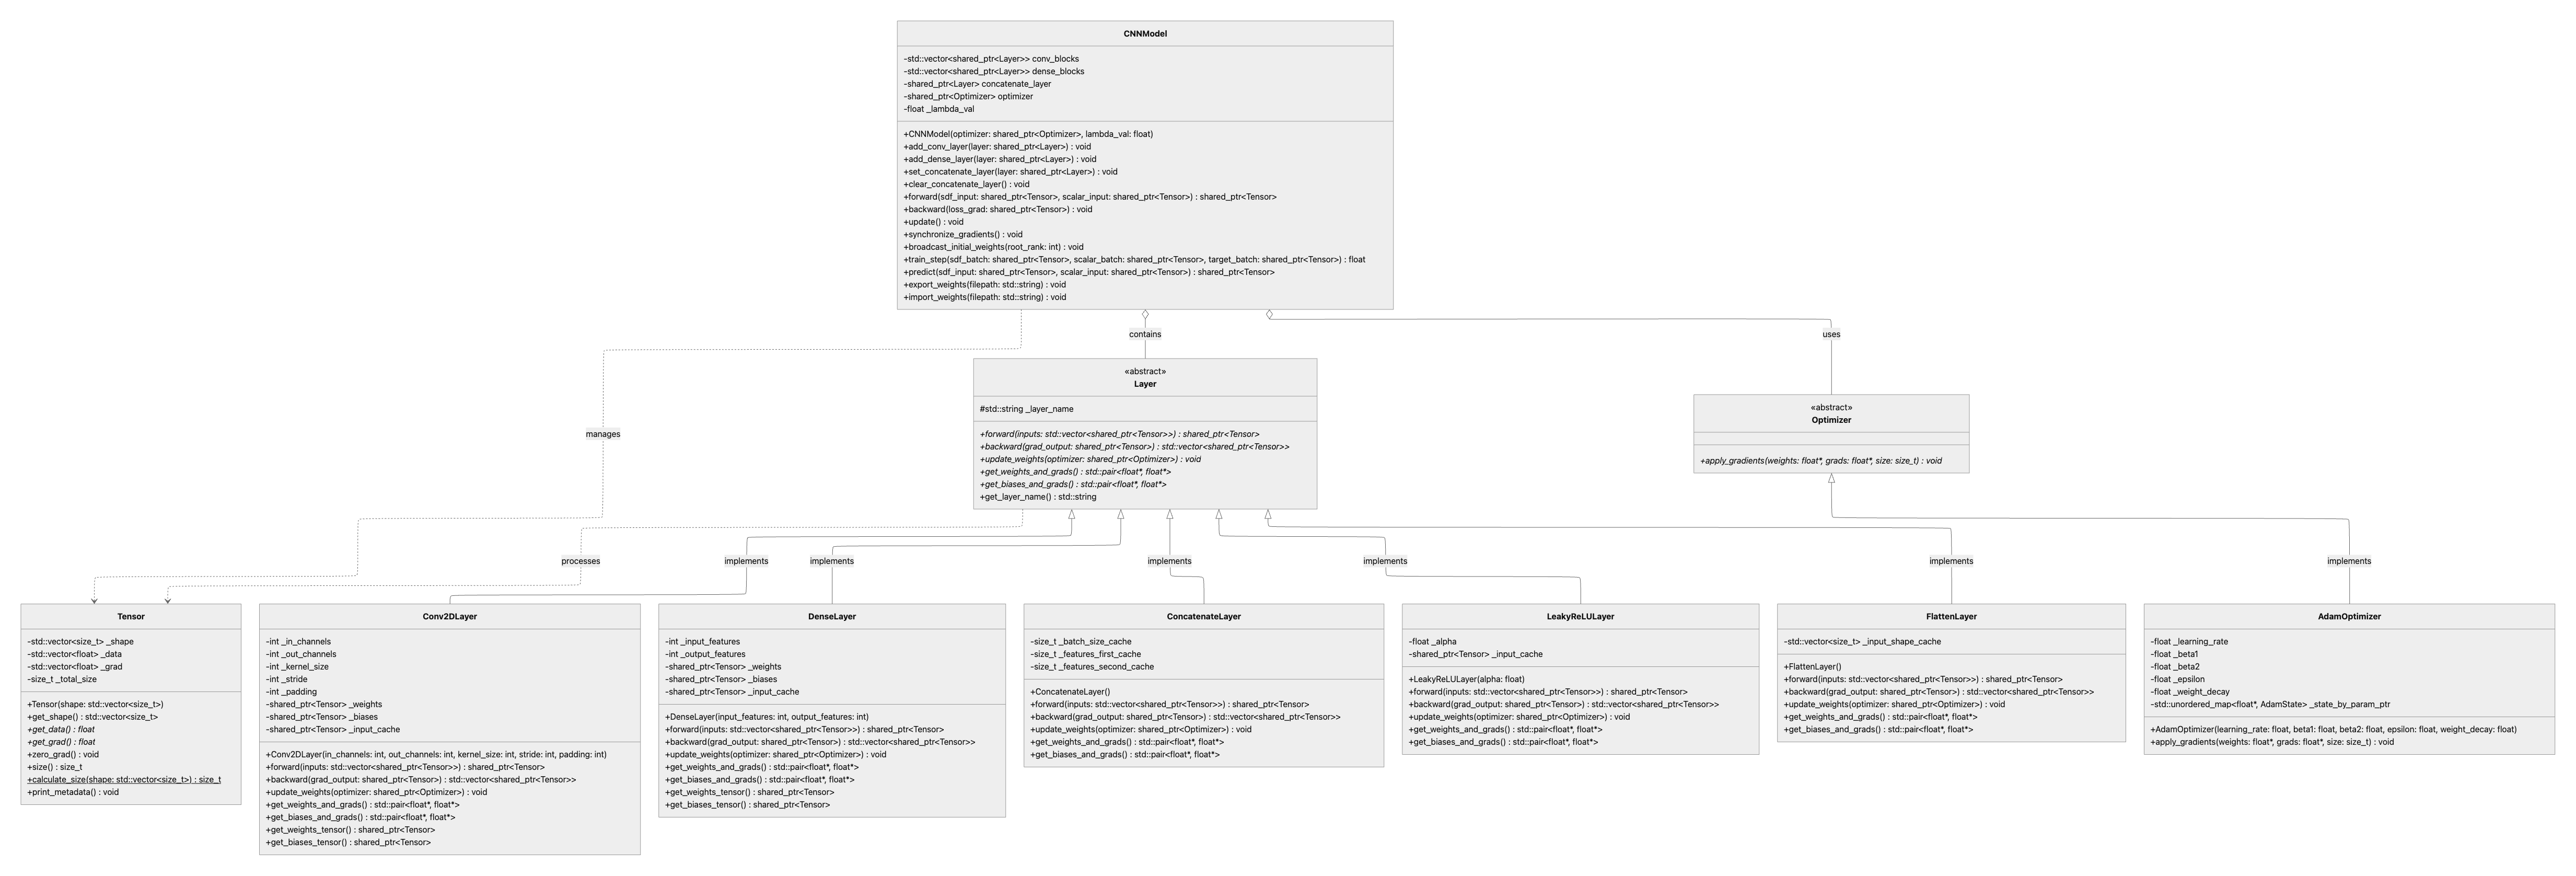
\includegraphics[width=1\linewidth]{Images/Chapter03/uml_diagram.png}
    \caption{UML class diagram illustrating the object-oriented design of the \cpp Convolutional Neural Network.}
    \label{fig:03_cnn_uml}
\end{figure}

In the following sections, we decide to highlight the most interesting implementations of these components, detailing key choices and memory optimization layouts, as well as providing an explanation of the core functions implemented.

\subsubsection{Geometric Preprocessing: SDF Generator}

The generation of the Signed Distance Function is encapsulated within the \texttt{SDFGenerator} class, which maps airfoil geometries to structured 2D tensors suitable for convolutional processing.\\

To maximize CPU cache efficiency and minimize cache misses during spatial calculations, boundary vertices are stored in a \texttt{std::vector<Point>}, where \texttt{Point} is a simple structure holding \texttt{x} and \texttt{z} coordinates. This choice creates a single contiguous array for the boundary data.\\

Upon initialization, the constructor ensures scale invariance (as detailed in Section \ref{sec:03_SDF}) by calling two private helper methods: \textbf{\texttt{computeCord()}} calculates the chord length $c$ using \texttt{std::hypot} to prevent numerical overflow\footnote{This function scales intermediate values before performing the sum of squares, avoiding the premature overflow or underflow that can occur when computing the norm directly as $\sqrt{\Delta x^2 + \Delta z^2}$} and \textbf{\texttt{normalizePoint()}} scales all vertex coordinates accordingly\footnote{This normalization step will be valuable for future implementations aimed at studying the effect of ice accumulation on the lift coefficient.}.\\

With a normalized boundary in place, the \texttt{SDFGenerator} computes the signed distance for each point on the target grid. This is achieved through a set of optimized geometric kernel functions:
\begin{itemize}
    \item[-] \textbf{\texttt{computeDistance(...) const}} calculates the minimum Euclidean distance from a grid point to a boundary segment (as it is shown in Equations \eqref{eq:03_orthogonal_projection} and \eqref{eq:03_clamping}). It includes a safety check for degenerate edges (where the two end-point of the segment coincide) to prevent division-by-zero errors;
    \item[-] \textbf{\texttt{getMinDistance(...) const}} iterates through all boundary edges of the airfoil, calling for each one \texttt{computeDistance} and returning the absolute minimum distance found. Additionally, we used \\\texttt{static\_cast<int>(airfoil.boundary.size())} to safely convert the unsigned vector size to a signed integer, preventing signed/unsigned comparison warnings;
    \item[-] finally, the \textbf{\texttt{windingAlgorithm(...) const}} implements the Winding Number Algorithm previously explained (Section \ref{sec:03_SDF}) to verify whether a grid point $p$ lies inside or outside the closed boundary. This is computed by analyzing edge crossings and using the 2D cross product (Equation \eqref{eq:cross_product})\footnote{Implemented through the \textbf{\texttt{crossProduct(Point p, Point a, Point b) const}} with each point passed by value, in order improve performance for small \texttt{structs} by allowing them to be passed directly in CPU registers, avoiding memory indirection.}, returning \texttt{true} if the point is inside the domain.
\end{itemize}
\vspace{2ex}

Once these values are computed for every grid point, the \textbf{\texttt{mappingToMatrix}} function converts the resulting 1D flattened SDF data into the required $150 \times 150$ 2D matrix format and writes it to a file, utilizing the \textbf{RAII (Resource Acquisition Is Initialization)} paradigm via \texttt{std::ofstream outfile(filename)} that automatically closes the file descriptor when \texttt{outfile} goes out of scope, in order to prevent system resource leaks in case of exceptions.\\

The most computationally intensive part of the process is executing these kernels for each one of the $150 \times 150 = 22,500$ points on the grid. This task is a classic example of an \textit{embarrassingly} parallel problem and it is implemented in the \texttt{generateTensorMPI} method, the details of which are provided in Section \ref{sec:03_parallelism}.

\subsubsection{Core abstractions and memory management}

To achieve high computational throughput while preserving a flexible design, the system introduces two core abstractions: a unified multi-dimensional tensor representation and a polymorphic layer interface.

\paragraph{Tensor}

The foundational data structure of our CNN implementation is the \texttt{Tensor} class, which manages both forward activation data (\texttt{\_data}) and backward gradients (\texttt{\_grad}) as multi-dimensional arrays of single-precision floating-point numbers.\\

First of all, the constructor \textbf{\texttt{Tensor(std::vector<size\_t> shape)}} initializes the shape descriptor and sets the \texttt{\_total\_size} member through a member \textbf{initializer list}. It pre-allocates and zero-initializes the storage vectors using \texttt{std::vector::resize}, that guarantees contiguous memory allocation. Direct access to this underlying memory is provided via the \texttt{get\_data()} and \texttt{get\_grad()} methods, which return raw pointers (\texttt{float*}) using the \texttt{.data()} member function.\\

Beyond raw pointer access, the class provides safe, native array-like indexing for flattened 1D elements through overloaded \texttt{operator[]} methods, offering both mutable and read-only (\texttt{const}-qualified) references. Utility functions are also optimized: gradient values are efficiently reset before each backward pass using the \texttt{std::fill} algorithm within the \texttt{zero\_grad()} method.\\

Furthermore, the total element count is computed by \texttt{calculate\_size()}, which is declared as a \texttt{static} method\footnote{This allows the method to be invoked without a class instance, for example, within a member initializer list.} and accepts a constant reference to avoid the overhead of copying the shape vector.\\

Finally, the class strictly adheres to \texttt{const} correctness, ensuring that utility methods like \texttt{print\_metadata()} are executed safely without modifying the object's internal state.

\paragraph{Layer}

The abstract base class \texttt{Layer}, defined in \texttt{Layer.hpp}, establishes a unified interface for all CNN components by leveraging runtime polymorphism to decouple the high-level network topology from the specific implementations of individual layers.\\

\textbf{Runtime polymorphism} is achieved through virtual functions and dynamic dispatch. When a class declares virtual methods, the compiler generates a virtual method table (\texttt{vtable}) containing pointers to these functions. Each object instance is implicitly equipped with a pointer (\texttt{vptr}) to its class's \texttt{vtable}. During execution, when a virtual method is called via a base class pointer, the program resolves the call dynamically: it dereferences the object's \texttt{vptr} to access the \texttt{vtable} and executes the overridden method corresponding to the actual derived type.\\

This mechanism is fundamental to our design. Rather than relying on conditional logic to handle the different mathematical operations, polymorphism allows the model to store and manage all layers uniformly within a single container (\texttt{std::vector<std::shared\_ptr<Layer>}). In addition, this design ensures high scalability and the effortless integration of new layer types simply by inheriting from the \texttt{Layer} base class.\\

Following the idea of implementing the polymorphism, we declared a virtual destructor \textbf{\texttt{\textasciitilde Layer() = default}}, ensuring that when a derived layer object is destroyed via a base class pointer, the derived class's destructor is executed, preventing resource leaks of dynamically allocated memory.\\

The core operations of the network are declared as pure virtual functions (indicated by the \texttt{= 0} suffix), which must be overridden by every concrete layer subclass. Specifically, we implemented:
\begin{itemize}
    \item[-] \textbf{\texttt{forward}}, that computes forward activations, and \textbf{\texttt{backward}}, that performs backpropagation, both accepting and returning \texttt{std::shared\_ptr} in order to guarantee automatic memory deallocation when the tensors are no longer needed;
    \item[-] \textbf{\texttt{get\_weights\_and\_grads()}} and \textbf{\texttt{get\_biases\_and\_grads()}} that returns \texttt{std::pair<float*, float*>} packaging the weight/bias arrays and their corresponding gradients into a single return value. Returning non-const pointers allows the optimizer to modify the parameter values directly in place.
\end{itemize}
\vspace{2ex}

Finally, architectural decoupling is achieved through a forward declaration of the \texttt{Optimizer} class; this resolves potential circular dependencies while allowing the \texttt{update\_weights(std::shared\_ptr<Optimizer>)} method to delegate parameter updates to external optimization algorithms seamlessly.

\subsubsection{Computational and activation layers}

The computational layers manage the network's mathematical transformations and contain all trainable parameters, while activation layers introduce the necessary non-linear activation boundaries.

\paragraph{DenseLayer}

The concrete \texttt{DenseLayer} class implements the fully-connected linear transformation $\mathbf{y} = W \mathbf{x} + \mathbf{b}$, where $W$ is the weight matrix and $\mathbf{b}$ is the bias vector, as described in details in the Section \ref{sec:03_dense_layer}.\\

First of all, the constructor \texttt{DenseLayer(int input\_features, int output\_features)} allocates the weight and bias tensors utilizing \texttt{std::make\_shared} rather than direct initialization via \\\texttt{std::shared\_ptr(new Tensor(...))}. While this last one forces two separate heap allocations\footnote{One for the object and one for its control block.}, \\\texttt{std::make\_shared} performs a \textbf{single contiguous memory allocation} for both the reference-counting control block and the managed \texttt{Tensor} object, in order to reduce heap fragmentation and improve CPU cache locality by keeping the control metadata and the tensor data adjacent in memory.\\

To ensure gradient stability at the start of training, the weights are initialized according to the \textbf{Xavier/Glorot scheme}, drawing from a uniform distribution bounded by $\pm\sqrt{6 / (N_{\text{in}} + N_{\text{out}})}$ using \texttt{std::default\_random\_engine} and \texttt{std::uniform\_real\_distribution<float>}.\\

During the \texttt{forward} pass, the input tensor is explicitly cached (\texttt{\_input\_cache}) to satisfy the mathematical requirements of backpropagation, as the input vector $\mathbf{x}$ must be retained to compute the weight updates as $\frac{\partial L}{\partial W} = \mathbf{x} \otimes \frac{\partial L}{\partial \mathbf{y}}$.\\

Moreover, the linear transformation $Y = X W^T + \mathbf{b}$ is evaluated through three nested loops:
\begin{itemize}
    \item[-] the outermost loop iterates over the batch size $b$;
    \item[-] the middle loop iterates over the output features $j$;
    \item[-] the innermost loop iterates over the input features $i$ to evaluate the dot product $Y_{b,j} = \sum_i X_{b,i} W_{j,i} + b_j$.
\end{itemize}
The weight matrix $W$ is stored in a transposed format of shape $(N_{\text{out}}, N_{\text{in}})$. This ensures that as the innermost loop increments its index over the input features, it accesses both the input tensor $X$ and the weight tensor $W$ with a unit stride. This design maximizes spatial locality, reduces cache misses, and enables the compiler to generate efficient SIMD vector instructions.\\

To conclude, also the \texttt{backward} method computes the gradients through three distinct sets of nested loops:
\begin{enumerate}
    \item the gradient with respect to the inputs is calculated as $dX_{b,i} = \sum_j dY_{b,j} W_{j,i}$. In this loop structure, the weight matrix is traversed column-wise, resulting in non-contiguous memory access;
    \item the gradient with respect to the weights is accumulated as $dW_{j,i} = \sum_b dY_{b,j} X_{b,i}$ using loops over $j$, $i$, and the batch dimension $b$. The innermost loop iterates over $b$, calculating the outer product of the output gradients and cached inputs;
    \item the gradient with respect to the biases is accumulated as $dB_j = \sum_b dY_{b,j}$ by summing the output gradients across all batch elements for each output feature.
\end{enumerate}

\paragraph{LeakyReLULayer}

The concrete \texttt{LeakyReLULayer} class implements homonymous element-wise activation function shown in Equation \eqref{eq:03_leaky_relu}. The negative slope parameter $\alpha$ is configured into the constructor \texttt{LeakyReLULayer(float alpha = 0.05f)}.\\

The interesting thing in this code is the use of the ternary operator:
\begin{itemize}
    \item[-] in the \texttt{forward} method, the element-wise activation is evaluated inside a contiguous loop using raw pointers \texttt{out\_ptr[i] = (in\_ptr[i] > 0.0f) ? in\_ptr[i] : \_alpha * in\_ptr[i]};
    \item[-] in the \texttt{backward} method, that is used to evaluate the gradient with respect to the input by scaling the output gradient as shown in Equation \eqref{eq:03_derivative_leaky_relu}, implemented as \texttt{din\_ptr[i] = dout\_ptr[i] * ((cache\_ptr[i] > 0.0f) ? 1.0f : \_alpha)}.
\end{itemize}
Because the derivative of the activation function is conditioned on the sign of the original input activations, caching the forward input tensor inside \texttt{\_input\_cache} is necessary to retrieve the values during the backward pass.\\

To conclude this class, because the activation layer contains no learnable parameters, the overridden method \texttt{update\_weights} is implemented as a no-op. Moreover, the parameter accessors \texttt{get\_weights\_and\_grads()} and \texttt{get\_biases\_and\_grads()} return a pair of type-safe null pointers, \texttt{\{nullptr, nullptr\}}.

\paragraph{Conv2DLayer}
\label{sec:03_conv}

The concrete \texttt{Conv2DLayer} class extends the abstract \texttt{Layer} interface to perform 2D spatial convolutions on four-dimensional tensors, which logically represent \textbf{batch samples, channels, height and width}.\\

Upon instantiation, the constructor initializes the convolutional kernels using a \textbf{Gaussian Xavier scheme} to ensure variance stability across deep network layers. The standard deviation for this distribution is computed as $\sigma = \sqrt{2 / (F_{\text{in}} + F_{\text{out}})}$, where the fan-in and fan-out dimensions are defined as $F_{\text{in}} = C_{\text{in}} \times K^2$ and $F_{\text{out}} = C_{\text{out}} \times K^2$, with $K$ denoting the kernel size.\\

During the \texttt{forward} pass, the spatial dimensions of the output tensor are explicitly calculated using Equation \eqref{eq:03_convol} and the resulting tensor is allocated contiguously via \texttt{std::make\_shared}. Because the system flattens all multi-dimensional tensors into 1D contiguous vectors for optimal memory layout, the layer utilizes a private inline helper function, \texttt{idx4}, to resolve 4D indices to 1D offsets. This enforces a strict row-major mapping:
\begin{equation}
    \text{Offset}(a, b, c, d) = \left[ \left( a \times \text{dim}_b + b \right) \times \text{dim}_c + c \right] \times \text{dim}_d + d
\end{equation}
where $a, b, c, d$ represent the target indices across the batch, channel, and spatial dimensions.\\

The forward convolution operation is executed through seven-nested loop. The outer four loops iterate over the batch elements $n$, output channels $oc$ and spatial output coordinates $oh$ and $ow$, while the inner three loops traverse the input channels $ic$ and kernel dimensions $kh$ and $kw$. To handle boundaries without incurring the overhead of allocating memory for physical zero-padding, the implementation uses implicit padding. Source coordinates are dynamically evaluated at each step as $ih = oh \times S + kh - P$ and $iw = ow \times S + kw - P$:
\begin{itemize}
    \item[-] if these fall outside the input boundaries, the multiplication is safely bypassed using a \texttt{continue} statement;
    \item[-] otherwise, the flattened indices are retrieved via \texttt{idx4}, and the kernel-input products are accumulated into a running sum initialized with the appropriate channel bias.
\end{itemize}
\vspace{2ex}

Finally, the \texttt{backward} method evaluates gradients using two distinct loop structures:
\begin{enumerate}
    \item[-] the first structure computes the parameter gradients: the bias gradient ($dB$) aggregates the output gradients directly, while the weight gradient ($dW$) accumulates the product of the output gradients and the cached forward inputs;
    \item[-] the second structure computes the gradient with respect to the input ($dX$) by performing a full convolution between the output gradients and the flipped kernel filters. To achieve this, the loop accesses the weights using inverted spatial coordinates:
    \begin{equation}
        kh_{\text{orig}} = K - 1 - kh, \quad kw_{\text{orig}} = K - 1 - kw
    \end{equation}
\end{enumerate}

\subsubsection{Structural Layers}

The \textbf{structural layers} are parameter-free components designed to rearrange and route data tensors across the branches of the network.

\paragraph{FlattenLayer}

The \texttt{FlattenLayer} class extends the base \texttt{Layer} interface to perform a logical reshaping of the 4D feature maps (generated by the convolutional branch) into a 2D tensor suitable for the subsequent \texttt{ConcatenateLayer}.\\

The \texttt{forward} method calculates the flattened size $F = C \times H \times W$ and allocates a 2D output tensor of shape $[B \times F]$ via \texttt{std::make\_shared}. Since the flatten operation is basically a reshape, the data is copied from the input to the output tensor sequentially in a single loop, preserving the element order across contiguous memory arrays.\\

The \texttt{backward} method receives the 2D gradient tensor \texttt{grad\_output} (of shape $[B \times F]$), validates the batch size consistency, allocates a 4D gradient tensor matching the cached shape \texttt{\_input\_shape\_cache}\footnote{This member attribute of type \texttt{std::vector<size\_t>} preserves the original spatial dimensions ($C \times H \times W$) to reconstruct and propagate the gradient back.} and performs the inverse sequential copy \texttt{grad\_in\_ptr[i] = grad\_out\_ptr[i]}, reconstructing the 4D gradient layout for the preceding convolutional layer.

\paragraph{ConcatenateLayer}

The \texttt{ConcatenateLayer} class is used to obtain a single tensor that combines the information from the \textbf{Convolutional Layer} and the scalar values of the Reynolds number and angle of attack.\\

Beyond the mathematical formalism about the shape of the matrices described in a detailed way in Section \ref{sec:03_struct_layer}, the merge operations are implemented with nested loops:
\begin{itemize}
    \item[-] the outer loop iterates over the batch size $n$, computing the row offsets for the first input \\(\texttt{n * \_features\_first\_cache}), the second input (\texttt{n * \_features\_second\_cache}) and the output (\texttt{n * (\_features\_first\_cache + \_features\_second\_cache)});
    \item[-] two inner loops then copy the data, ensuring row-wise contiguous layout. 
\end{itemize}
\vspace{2ex}
During the \texttt{backward} method, this operation is inverted. The layer receives a combined gradient tensor of shape $[B \times (D_1 + D_2)]$ and must route the gradients back to their respective origins, reversing the copy logic: for each batch element, it copies the first $D_1$ components of the output gradient to the first input gradient buffer and the remaining $D_2$ components to the second input gradient buffer. Both elements are then returned in a standard vector \texttt{\{grad\_first, grad\_second\}}.

\subsubsection{Training pipeline, loss and optimizers}

The network's optimization and training pipeline is coordinated by mathematical loss functions and state-tracking optimization solvers.

\paragraph{Loss}

Unlike the object-oriented structure of the computational layers, the \textbf{physics-informed loss function} and its corresponding gradient are implemented as non-member utilities within the \texttt{Loss} namespace. This design choice avoids the overhead of object instantiation and maintains a functional style for stateless operations.\\

In the \texttt{forward} method\footnote{That accepts predictions, targets and angles of attack (\texttt{alphas}) tensors as \texttt{const std::shared\_ptr<Tensor>\&}.}, the composite physics-informed loss, described in Section \ref{sec:03_loss}, is computed in a single loop using raw pointers retrieved via \texttt{get\_data()} to ensure contiguous memory traversal. When computing the physics-informed penalty, the masking logic from Equation \eqref{eq:03_mask} is applied: the linear regime limit is saved in an anonymous namespace at the beginning of the file, in order to restrict the scope of this constant. The average data and physics terms are computed and normalized by the number of elements using \texttt{static\_cast<float>(n)}\\

Finally, the \texttt{backward} method is implemented in a similar way.

\paragraph{Optimizer and Adam Optimizer}

Similar to the layer architecture, the optimization logic is strictly decoupled from the neural network topology via an abstract \texttt{Optimizer} base class. This unified interface ensures that different numerical solvers can be swapped seamlessly, exposing a single pure virtual function (\texttt{apply\_gradients(float* weights, float* grads, size\_t size)}) to handle dynamic dispatch interface that must be implemented by concrete subclasses.\\

The only concrete implementation of this interface is the \texttt{AdamOptimizer}, which executes the \textbf{Adaptive Moment Estimation} algorithm detailed in Section \ref{sec:03_adam}.\\

To map specific weight and bias arrays to their corresponding optimization states without coupling the layers to the optimizer, the class utilizes a parameter-to-state lookup map as \texttt{std::unordered\_map<float*, AdamState> \_state\_by\_param\_ptr}\footnote{Where \texttt{AdamState} is a private structure that contains the first moment vector \texttt{std::vector<float> m}, the second moment vector \texttt{std::vector<float> v}, and an unsigned integer \texttt{timestep} to keep track of the parameter update steps.}, that provides average constant-time $\mathcal{O}(1)$ lookup complexity. Since weight and bias arrays are allocated once and reside in contiguous memory locations throughout the lifetime of the network, their raw memory addresses (\texttt{float*}) serve as unique keys. This pointer-based hashing avoids the overhead of index-based tracking or string-based lookups and enables on-the-fly initialization of the \texttt{AdamState} upon the first optimization step.

\paragraph{CNNModel}
\label{sec:03_CI_CNN}

The concrete class \texttt{CNNModel} coordinates the execution, training and state management of the entire neural network. It aggregates the layers of the convolutional branch and the dense branch, manages feature fusion, interfaces with the optimizer and implements utilities for distributed data-parallel training and weight serialization.\\

The \texttt{forward} method propagates input tensors sequentially through the model. To maximize efficiency, the iteration over the layer containers (\texttt{conv\_blocks} and \texttt{dense\_blocks}) utilizes \texttt{const auto\&}, thereby avoiding the performance overhead associated with incrementing reference counters on the underlying shared pointers. Conversely, the \texttt{backward} method employs reverse iterators to correctly propagate gradients upstream in strict accordance with the chain rule.\\

Another interesting detail is that in the \texttt{update} method gradient values are clipped to the interval $[-1.0, 1.0]$ to prevent gradient explosion\footnote{This choice has been made after training the model for the first time, where we have noticed very strong fluctuations of the loss value during the training process.}. This is executed via a local lambda function (\texttt{clip\_layer}) containing a nested \texttt{clip\_tensor} lambda, which directly modifies the elements in-place using standard pointer-based loops. \\

Whenever layer-specific parameters must be accessed for weight updates, gradient synchronization, or serialization, the model dynamically resolves the abstract base pointer types through runtime downcasting via \texttt{std::dynamic\_pointer\_cast} (e.g., casting from \texttt{std::shared\_ptr<Layer>} to \texttt{std::shared\_ptr<Conv2DLayer>}).\\

Finally, the model implements binary weight export and import methods using \texttt{std::ofstream} and \texttt{std::ifstream}, opened with the \texttt{std::ios::binary} flag. Binary data is written and read directly via type-unsafe low-level operations utilizing \texttt{reinterpret\_cast<const char*>} and \texttt{reinterpret\_cast<char*>} to map raw byte buffers, which minimizes I/O latency. During the import phase, after reading the shapes and element counts from the file, weight vectors are populated using \texttt{std::move} (from the \texttt{<utility>} header) to transfer the ownership of heap-allocated arrays into the target structures, bypassing expensive memory allocation and copying. To illustrate this efficient binary format, Table \ref{tab:weights_header_example} details the layout of the file header and the metadata corresponding to the initial \texttt{Conv2DLayer}.

\begin{table}[h!]
  \centering
  \caption{Example layout of the binary weight file header, showing the global count of layers followed by the name and weight/bias tensor metadata of the first layer (\texttt{Conv2DLayer}).}
  \label{tab:weights_header_example}
  \begin{tabular}{lll}
    \hline
    Byte Offset & Field Name & Value / Example \\
    \hline
    \texttt{0x00--0x07}   & Total layers in model ($N_{\text{layers}}$) & \texttt{8} \\
    \texttt{0x08--0x0F}   & Layer name length ($L_{\text{name}}$) & \texttt{39} \\
    \texttt{0x10--0x36}   & Layer name string & \texttt{"Conv2DLayer(1,8,5, stride=5, padding=0)"} \\
    \texttt{0x37}         & Weights presence flag & \texttt{true} (\texttt{0x01}) \\
    \texttt{0x38--0x3F}   & Weights tensor rank ($R_W$) & \texttt{4} \\
    \texttt{0x40--0x5F}   & Weights tensor shape & \texttt{[8, 1, 5, 5]} \\
    \texttt{0x60--0x67}   & Total weights count ($N_W$) & \texttt{200} \\
    \texttt{0x68--0x387}  & Weights raw data & \texttt{[-0.0125, 0.0841, \dots]} \\
    \texttt{0x388}        & Biases presence flag & \texttt{true} (\texttt{0x01}) \\
    \texttt{0x389--0x390} & Biases tensor rank ($R_B$) & \texttt{1} \\
    \texttt{0x391--0x398} & Biases tensor shape & \texttt{[8]} \\
    \texttt{0x399--0x3A0} & Total biases count ($N_B$) & \texttt{8} \\
    \texttt{0x3A1--0x3C0} & Biases raw data & \texttt{[0.0, 0.0, \dots]} \\
    \hline
  \end{tabular}
\end{table}

\subsubsection{Data Pipelines: \texttt{NPZDataLoader}}

The \texttt{NPZDataLoader} class manages the retrieval, normalization, and partitioning of datasets stored in the compressed NumPy (\texttt{.npz}) format. This format was explicitly selected because it packages multiple named multidimensional arrays within a single ZIP archive, acting as an efficient bridge between Python-based preprocessing scripts (such as \texttt{build\_dataset.py}) and the \cpp training pipeline without the severe parsing overhead of text-based formats like CSV.\\

Specifically, the dataset is structured into four core arrays:
\begin{itemize}
    \item[-] \texttt{X\_sdf}, representing the $150 \times 150$ SDF of the airfoil geometries;
    \item[-] \texttt{X\_scalars}, storing the Reynolds number ($\mathrm{Re}$) and the angle of attack ($\alpha$);
    \item[-] \texttt{Y\_cl}, containing the ground-truth lift coefficient ($C_L$) labels computed from the Navier-Stokes simulations;
    \item[-] \texttt{metadata}, containing the specific NACA airfoil profile labels.
\end{itemize}
This class provides a complete input pipeline, converting these raw data arrays into normalized, formatted tensor batches for network training.\\

To import the data without introducing heavy external \cpp NumPy parsing libraries, the internal reading method establishes a read-only POSIX pipe to execute a brief Python script, that utilizes Python's native numpy library to load the specified array, converts it to raw single-precision bytes and streams the output directly to the standard output. The \cpp program then intercepts this byte stream, reading it sequentially into a standard vector buffer before safely closing the process and verifying its exit status.\\

Once the arrays are loaded into memory, the constructor applies Z-score standardization across the SDF, scalar parameters and target lift coefficients, to prevent numerical instability during the training phase. Then, the class handles the sequential feeding of this data during training. The batching process partitions the normalized dataset into mini-batches by maintaining an internal cursor that tracks the current read position. For each requested batch, it allocates new tensor objects and utilizes standard library copying algorithms to transfer the exact slice of data from the internal buffers to the newly created tensors.

\subsubsection{Main execution of the CNN}

The main execution entry point of the neural network workflow is defined in \texttt{main.cpp}. It coordinates the loading of datasets, the structural composition of the CNN layers and the training and validation loops over successive epochs.\\

The program begins by instantiating the training and testing pipelines using \texttt{NPZDataLoader} to load the compressed NumPy datasets. It then creates a shared instance of the \texttt{AdamOptimizer} wrapped in a \texttt{std::shared\_ptr} via \texttt{std::make\_shared} with a designated learning rate of $10^{-5}$. This optimizer is passed to initialize the \texttt{CNNModel} instance.\\

The architecture of the neural network is composed using the model's builder methods:
\begin{enumerate}[itemsep=2ex, topsep=2ex]
    \item the convolutional branch is constructed by adding a \texttt{Conv2DLayer} with 1 input channel, 8 output channels, a $5 \times 5$ kernel, and a stride of 5, followed by a \texttt{LeakyReLULayer} (with an activation slope $\alpha = 0.05$) and a \texttt{FlattenLayer} to reduce the spatial feature maps to a one-dimensional representation of size 7200;
    \item the feature fusion stage is enabled by registering a \texttt{ConcatenateLayer} via \texttt{set\_concatenate\_layer()}, which merges the geometry features with the two physical flow parameters (Reynolds number and angle of attack);
    \item the fully-connected regression head is built using three sequential \texttt{DenseLayer}s of dimensions $7202 \to 128$, $128 \to 64$, and $64 \to 1$, separated by \texttt{LeakyReLULayer} activations, resulting in a single scalar prediction representing the lift coefficient ($C_L$).
\end{enumerate}
\vspace{2ex}
The training process iterates for 100 epochs. Within each epoch, it resets the data loaders and processes the dataset in mini-batches. For each batch, it invokes \texttt{train\_step} on the model instance to run the forward pass, evaluate the PINN loss function, compute parameter gradients via backpropagation and update the weights. After the training phase of each epoch, it runs a validation pass by propagating the validation samples through the network via \texttt{forward()} to monitor generalization and check for overfitting by computing the MSE against the validation targets.

% ===================================================================
% PARALLELISM AND SCALABILITY
% ===================================================================

\subsection{Parallelism}
\label{sec:03_parallelism}

To achieve high-performance capabilities and scale the computational workflow to large-scale grids and datasets, the codebase employs distributed-memory parallelism using the \textbf{Message Passing Interface (MPI)} standard. The parallelization strategy is implemented at two distinct stages: the geometric preprocessing phase (for parallel SDF generation) and the neural network training phase (for distributed data-parallel training).

\subsubsection{Parallel SDF Generation}

The computation of the SDF, as described in Section \ref{sec:03_SDF}, is an embarrassingly parallel task, since the evaluation of the signed distance for each point on the $150 \times 150$ grid is independent of all other points.\\

To do this, upon initializing the MPI environment via \texttt{MPI\_Init}, the total number of grid points ($N_{\text{total}} = 22,500$) is partioned by the communicator size ($S$, retrieved using \texttt{MPI\_Comm\_size}). Because there could be some cases where $N_{\text{total}}$ is not perfectly divisible by $S$, the remainder ($R = N_{\text{total}} \bmod S$) is distributed among the first $R$ processes\footnote{This partitioning guarantees perfect load balancing, as the workload of any two processes differs by at most a single grid point.}. Each process (with rank ID $r$, retrieved via \texttt{MPI\_Comm\_rank}) computes its local count and offset as:
\begin{equation}
    N_{\text{local}} = \lfloor N_{\text{total}} / S \rfloor + \mathbb{I}(r < R)\quad\text{and}\quad O_{\text{local}} = r \lfloor N_{\text{total}} / S \rfloor + \min(r, R)
\end{equation}
where $\mathbb{I}$ is the indicator function.\\

Each process independently computes the SDF values for its assigned local grid points. To reconstruct the complete 2D matrix, the local chunks must be gathered into a global vector of size $N_{\text{total}}$, using \texttt{MPI\_Allgatherv}, which performs a vector gather-to-all communication. The collective call requires \texttt{recvcounts}, which stores the number of elements expected from each rank, and \texttt{displs}, which specifies the starting byte displacement of each segment in the global buffer. \texttt{MPI\_Allgatherv} ensures that all processes receive the full SDF image.\\

Finally, the root process (rank 0) writes the complete matrix to disk via the \texttt{mappingToMatrix} method, while other ranks proceed to the next file or terminate safely via \texttt{MPI\_Finalize}.

\subsubsection{Distributed Data-Parallel Training}

The training of the Convolutional Neural Network is parallelized in \texttt{CNN/main.cpp} and \texttt{CNNModel.cpp} using a data-parallel training strategy to scale to large datasets and decrease training epoch time.\\

In \texttt{CNN/main.cpp}, data parallelism is implemented by distributing the training batch across multiple processes. The global mini-batch size is scaled according to $B_{\text{global}} = B_{\text{local}} \times S$, with a local batch size of $B_{\text{local}} = 64$. To prevent redundant memory duplication, each process uses a custom \texttt{slice\_batch\_tensor} method to extract only its specific segment of the global dataset, beginning at the index offset $r \times B_{\text{local}}$.\\

To guarantee consistent optimization across the distributed environment, the training pipeline enforces MPI synchronization at three critical stages:
\begin{enumerate}[itemsep=2ex, topsep=2ex]
    \item initially, the root process generates the network weights and distributes them to all other ranks using \texttt{MPI\_Bcast} on the raw tensor buffers, ensuring an identical starting state\footnote{With all the weights initialized to the same value.} across the entire communicator;
    \item during the backpropagation phase, each process computes gradients based on its local batch slice. Before applying the Adam optimization step, these local gradients are aggregated via an in-place \texttt{MPI\_Allreduce} operation. By utilizing the \texttt{MPI\_SUM} operator directly on the existing memory buffers, the system efficiently avoids redundant data allocations. The accumulated gradients are then divided by the total number of processes $S$ to compute a global average, which guarantees that every rank applies the exact same mathematical update to its local parameters;
    \item finally, at the conclusion of each epoch, the local training losses, validation losses, and processed sample counts are gathered back to the root process via \texttt{MPI\_Reduce}, allowing it to calculate and report the consolidated global statistics.
\end{enumerate}

% ===================================================================
% RESULTS
% ===================================================================

\subsection{Results}

Given the significant model size of 930,513 trainable parameters, performing the training process on standard personal computers was computationally impractical within a reasonable timeframe. To overcome this limitation, the training was conducted on the high-performance computing (HPC) resources of the \textbf{CINECA Leonardo cluster}. Specifically, we utilized a full single node configured with two Intel Xeon Platinum 8480+ (Sapphire Rapids) processors, providing a total of 112 physical cores, backed by 512 GiB of DDR5 RAM operating at 4800 MHz. This hardware acceleration reduced the total execution time from several hours to approximately five minutes.\\

\begin{lstlisting}[style=bashstyle,
  caption={SLURM run script for CNN training (\texttt{run\_cnn.sh}).},
  label={lst:job_run}]
#!/bin/bash
#SBATCH --job-name=cnn_training
#SBATCH --account=EUHPC_D35_025
#SBATCH --partition=dcgp_usr_prod
#SBATCH --nodes=1
#SBATCH --ntasks-per-node=1
#SBATCH --cpus-per-task=112
#SBATCH --time=01:00:00
#SBATCH --output=cnn_%j.out
#SBATCH --error=cnn_%j.err


cd /leonardo/home/userexternal/gdonnine/CNN/Ice_acceleration_model_on_airplane_wing/CNN

module purge
module load python/3.11.7
module load gcc/11.3.0
module load intel-oneapi-compilers
module load intel-oneapi-mpi

srun ./cnn_mpi_executable
\end{lstlisting}

The network was trained for 100 epochs on a synthetically generated dataset of 2D SDF, representing five \textbf{symmetric NACA airfoil profiles} (NACA 0006, 0008, 0010, 0012 and 0018) across varying angles of attack ($\alpha$) and Reynolds numbers ($\mathrm{Re}$). Partitioned via an 80/20 split, the dataset yielded 1,713 training samples and 429 validation samples\footnote{All of which have been made publicly available on \href{https://www.kaggle.com/datasets/giulioenzodonninelli/sdf-symmetric-airfoil-high-reynolds-number}{\textcolor{blue}{Kaggle}}}.

\paragraph{Initial Unstable Training Run}

In our first training attempt, we adopted a standard learning rate of $10^{-3}$, without applying input feature normalization or gradient clipping. This configuration resulted in severe numerical instability during the optimization process. As illustrated in Figure \ref{fig:incorrect_training}, the training and validation losses exhibit chaotic, erratic oscillations, fluctuating wildly by over seven orders of magnitude (ranging from $10^{-1}$ to $10^6$ in log scale). The presence of massive loss spikes\footnote{Such as the prominent peaks around epochs 40, 60, 70 and 85.} is a clear indicator of exploding gradients. Without gradient clipping, large backpropagated gradients led to excessive parameter updates, pushing the weights into unstable regions of the loss landscape and preventing the optimizer from settling into a local minimum.

\begin{figure}[h!]
  \centering
  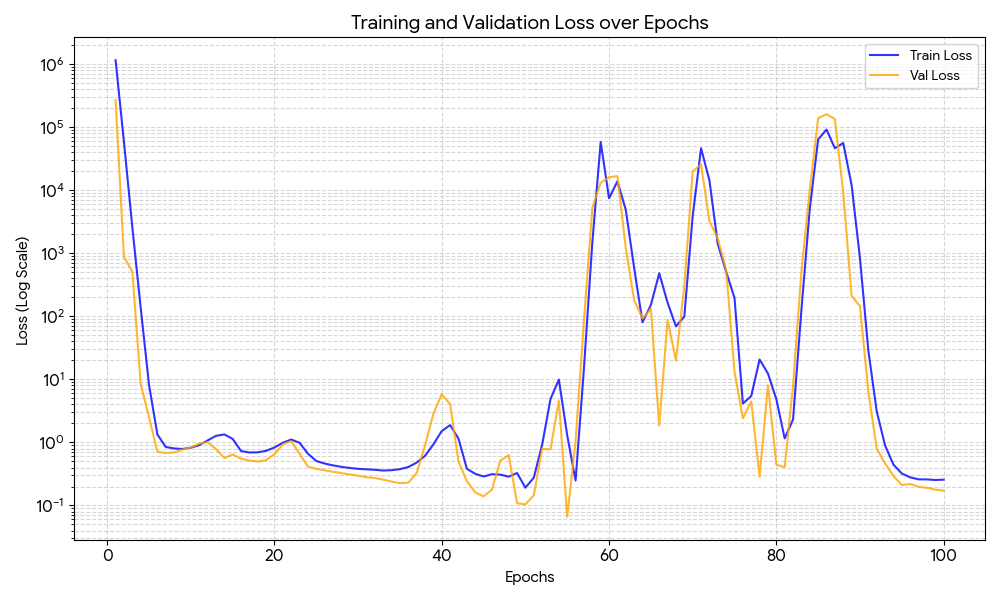
\includegraphics[width=0.70\linewidth]{Images/Chapter03/Incorrect_training.png}
  \caption{Log-scale evolution of the training and validation losses over 100 epochs during the initial unstable training attempt. The extreme oscillations and sudden spikes up to $10^6$ highlight the numerical instability caused by an excessively high learning rate and the absence of gradient clipping or feature normalization.}
  \label{fig:incorrect_training}
\end{figure}

\paragraph{Optimized Successful Training Run}

To resolve the numerical instability and ensure smooth convergence, three key modifications were implemented in the training pipeline:
\begin{enumerate}
    \item the Adam optimizer's learning rate ($\eta$) was reduced from $10^{-3}$ to $10^{-5}$;
    \item standard Z-score normalization was applied during the data-loading phase to scale the inputs (SDF and physical scalars) and targets (lift coefficients) to zero-mean and unit-variance;
    \item gradient clipping was enabled in the update phase to clamp all gradient components strictly within the interval $[-1.0, 1.0]$ (as detailed in Section \ref{sec:03_CI_CNN}).
\end{enumerate}
These modifications successfully stabilized the training trajectory.\\

As shown in Figure \ref{fig:correct_training}, the loss curves exhibit highly stable, monotonic convergence. The left plot (Full View) shows the rapid decay of the loss during the initial epochs, indicating that the network quickly learned the dominant physical relationships. The right plot (Zoomed View, Epochs 5-100) highlights the smooth, continuous reduction of both training and validation losses, with no signs of overfitting. The validation loss consistently tracks slightly lower than the training loss; this is a common characteristic when model regularization (such as L2 weight decay) is active during training or when the z-score normalization effectively centers the distribution of test cases.\\

This optimized training process completed in likely 5 minutes and 11 seconds, achieving a final training loss of 0.0104216 and a validation loss of 0.00784775, demonstrating both the efficiency and accuracy of our implementation.

\begin{figure}[h!]
  \centering
  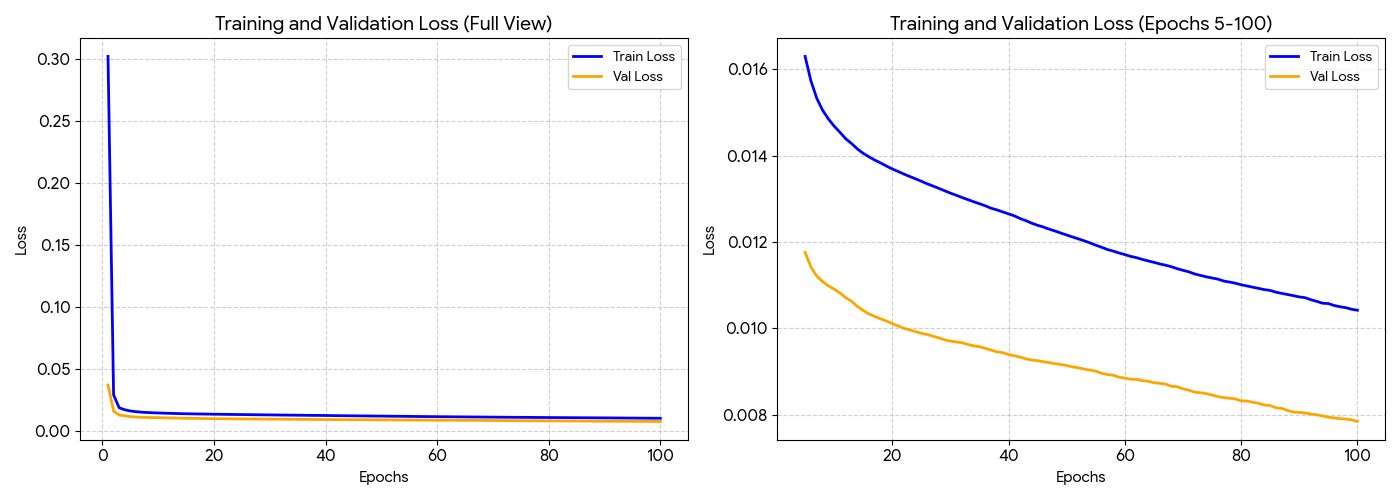
\includegraphics[width=0.85\linewidth]{Images/Chapter03/Correct_training.png}
  \caption{Evolution of training and validation losses for the optimized training run. The full view (left) illustrates the rapid initial convergence, while the zoomed-in view from epoch 5 to 100 (right) highlights the smooth, monotonic decrease of both metrics, confirming the effectiveness of Z-score normalization and gradient clipping.}
  \label{fig:correct_training}
\end{figure}

%-----------------------------------------------------------------------------
% Tuning
%-----------------------------------------------------------------------------

\section{Tuning}
\label{sec:04_Tuning}

The Convolutional Neural Network described and implemented in Chapter~\ref{sec:03_Convolutional_Neural_Network} provides the starting point for the numerical study presented in this chapter. Although the initial model is already able to approximate the lift coefficient from the airfoil geometry and the flow parameters, our objective is not limited to obtaining a working implementation. We also want to understand which choices of architecture, optimization algorithm, regularization, activation function, and learning rate allow the surrogate model to obtain more accurate and more reliable predictions. For this reason, we performed a sequence of controlled tuning experiments. In each experiment one group of quantities was varied, while the other settings were kept fixed as far as the corresponding driver allowed. The results were then analysed not only through the final validation error, but also through the evolution of the training objective, the physical validation error, the gradient norms, the actual parameter updates, and the activation distributions.

The order of the study follows the development of the model. First, we investigated the topology of the network, because the feature representation and the capacity of the regression head influence every subsequent experiment. We then considered dropout, the optimizer, the weight of the SIMM physical term, and L1 and L2 regularization. Once these settings had been examined, we compared the available activation functions and finally studied both the magnitude and the schedule of the learning rate. The last part of the chapter describes the long ordinary training run performed with the production executable and collects the conclusions that can be drawn from the complete tuning campaign.

\subsection{Cross-validation and diagnostic methodology}
\label{sec:04_cross_validation}

All the tuning experiments use the training dataset stored in \texttt{dataset/cnn\_dataset\_train.npz}, which contains 1713 samples. Each sample consists of a $150\times150$ Signed Distance Function, the scalar pair $(\mathrm{Re},\alpha)$, and the corresponding lift coefficient $C_L$. The separate file \texttt{dataset/cnn\_dataset\_test.npz}, containing 429 samples, is not used to compare candidates. In the intended procedure, it is loaded only after a candidate has been selected and the selected model has been refitted on the complete training dataset. This separation is important because using test data during the search would turn the final error into a selection quantity rather than an independent estimate.

The comparisons are performed with the project implementation of \texttt{RandomKFold}. The samples are shuffled with seed $42$ and divided into five folds. The splitter works at sample level, rather than keeping all observations belonging to one airfoil in the same fold. Consequently, the experiment measures interpolation over the sampled dataset and does not constitute a strict test of generalization to an entirely unseen airfoil family. In every fold, approximately eighty percent of the samples are used for training and the remaining twenty percent for validation. In the recorded runs, the validation sets contain 342 or 343 samples and the training sets contain 1370 or 1371 samples. The fold plan is generated once and reused for every candidate within a tuning experiment, so two candidates are compared on exactly the same validation observations.

Before a fold is trained, the normalization statistics are fitted only on that fold's training indices. The same statistics are subsequently applied to the corresponding validation samples. The angle of attack is read in degrees from the scalar input and converted to radians before it is used in the SIMM residual. Every candidate and every fold constructs a fresh model and a fresh optimizer. Therefore, neither the weights, the activation caches, nor the optimizer moments are transferred from another candidate or fold. The distributed training uses a global batch size, so changing the number of MPI ranks changes the distribution of the work but not the nominal batch size or the definition of the metrics.

The primary selection quantity is the physical-unit mean squared error on the validation samples. If $\widehat{C}_{L,i}$ is the predicted coefficient and $C_{L,i}$ is the CFD value, the physical MSE of fold $k$ is
\begin{equation}
    \mathrm{MSE}_{\mathrm{val}}^{(k)} =
    \frac{1}{n_k}\sum_{i\in\mathcal{V}_k}
    \left(\widehat{C}_{L,i}-C_{L,i}\right)^2,
    \label{eq:04_validation_mse}
\end{equation}
where $\mathcal{V}_k$ is the validation subset and $n_k$ is its number of samples. The candidate score is the sample-weighted aggregation returned by \texttt{CrossValidator}, rather than a comparison of the standardized SIMM objective. This distinction matters because the training objective contains a data term and, in some experiments, a physics term expressed in fold-specific standardized target units, whereas Equation~\eqref{eq:04_validation_mse} is expressed in the squared physical lift-coefficient units. The fold standard deviation is reported together with the mean to show the sensitivity to the data split.

The training objective is monitored through \texttt{train\_objective}, while the physical training and validation errors are read from \texttt{epoch\_metrics.csv}. The public cross-validation history is normally stored every ten epochs, although diagnostics contain a validation value at every epoch. The following diagnostic quantities are used throughout the chapter. The gradient norm is read from rows with \texttt{parameter\_scope=all}; it is measured after the MPI weighted gradient aggregation and before clipping and the optimizer update. The parameter update ratio is the actual movement of the parameters relative to their norm,
\begin{equation}
    r_{\theta} =
    \frac{\lVert\theta_{\mathrm{after}}-\theta_{\mathrm{before}}\rVert_2}
    {\max\left(\lVert\theta_{\mathrm{before}}\rVert_2,10^{-12}\right)},
    \label{eq:04_update_ratio}
\end{equation}
and is not simply a learning rate multiplied by a gradient. It includes the optimizer moments, clipping, decay, the numerical epsilon, and the current parameter values. Finally, activation statistics are distinguished between the pre-activation tensor entering a non-linearity and the post-activation tensor returned by it. Their mean, variance, minimum, maximum, and fixed-bin histograms are used to identify signal attenuation, saturation, or growth of the activation scale. In all cases, we checked the raw CSV files for non-finite values and for late-epoch increases before describing a run as numerically stable.

\subsection{Topology tuning}
\label{sec:04_topology_tuning}

The first tuning activity concerned the topology because the convolutional trunk determines how the $150\times150$ SDF is compressed, while the dense head determines how the geometric representation is combined with the two scalar flow parameters. A model that is too small may not represent the dependence of $C_L$ on geometry and angle of attack, whereas a model that is unnecessarily large may increase the number of trainable parameters without improving generalization. The experiment therefore varied the convolutional kernel size and the widths and depth of the dense head while keeping the optimizer, loss weight, training budget, and fold plan fixed. This type of structural comparison is also consistent with the surrogate-model motivation introduced in Chapter~\ref{sec:03_Convolutional_Neural_Network} and with the role of activation and gradient propagation in deep networks discussed by Glorot and Bengio~\cite{glorot2010understanding}.

For a two-dimensional convolution with input size $H_{\mathrm{in}}\times W_{\mathrm{in}}$, kernel size $K$, stride $S$, and zero padding $P$, the output dimensions are
\begin{equation}
    H_{\mathrm{out}} = \frac{H_{\mathrm{in}}-K+2P}{S}+1,
    \qquad
    W_{\mathrm{out}} = \frac{W_{\mathrm{in}}-K+2P}{S}+1.
    \label{eq:04_topology_convolution}
\end{equation}
The topology experiment used $P=0$ and set the stride equal to the kernel size. The $5\times5$ alternative consequently produces eight feature maps of size $30\times30$, or 7200 flattened features. After concatenation with the two scalar inputs, the first dense layer receives 7202 values. A head with widths $(w_1,\ldots,w_m)$ then applies successive transformations $\mathbf{h}_{j+1}=\sigma(W_j\mathbf{h}_j+\mathbf{b}_j)$ and ends with a linear scalar output. Increasing the widths mainly increases the capacity of the first dense transformation, while adding hidden layers changes the depth of the nonlinear mapping.

The search contained 18 candidates and therefore 90 fold evaluations. Each fold was trained for 100 epochs with global batch size 64, Adam at learning rate $10^{-5}$, SIMM physics weight $0.25$, LeakyReLU with negative slope $0.05$, and seed 42. The baseline was \texttt{conv5x5-dense-128-64}. The candidate selection was based on physical validation MSE, and the untouched test set was evaluated only after refitting the winning topology on all 1713 training samples.

\begin{table}[h!]
    \centering
    \begin{tabular}{lcc}
        \hline
        Candidate & Mean validation MSE & Fold standard deviation \\
        \hline
        \texttt{conv5x5-dense-1024-512-256-128} & 0.004560 & 0.000946 \\
        \texttt{conv5x5-dense-1024-512-256-128-64} & 0.004626 & 0.000918 \\
        \texttt{conv5x5-dense-1024-512} & 0.004851 & 0.000911 \\
        \texttt{conv5x5-dense-512-256-128-64} & 0.004872 & 0.001125 \\
        \texttt{conv5x5-dense-512-256} & 0.005052 & 0.001067 \\
        \texttt{conv5x5-dense-128-64} (baseline) & 0.006010 & 0.000823 \\
        \texttt{conv3x3-dense-512-256} & 0.006459 & 0.001318 \\
        \hline
    \end{tabular}
    \caption{Representative topology candidates selected from the complete 18-candidate grid.}
    \label{tab:04_topology_results}
\end{table}

The lowest observed validation MSE was obtained by \texttt{conv5x5-dense-1024-512-256-128}, with $0.004560\pm0.000946$. It improved on the baseline in all five folds. The refit of this topology produced an untouched-test MSE of $0.002805$. The result is not explained by depth alone. At width $(512,256)$, increasing the head from two to four hidden layers reduced the mean error from $0.005052$ to $0.004872$, while at width $(1024,512)$ the corresponding increase in depth reduced it from $0.004851$ to $0.004560$. Increasing width also helped at fixed depth, but the gains became smaller and then reversed: the depth-two sequence from $(512,256)$ to $(1024,512)$ improved the score, while the wider $(1536,768)$ and $(2048,1024)$ candidates became worse. The selected depth is therefore interior to the tested depth range, while its first-layer width is at the upper boundary of the grid. It is more accurate to describe the choice as the result of a moderate interaction between capacity and depth than to attribute it to one of these quantities alone.

The kernel comparison gives a second clear result. The $5\times5$ convolution was better than the corresponding $3\times3$ convolution in each paired comparison available in the grid. For the $(128,64)$, $(256,128)$, and $(512,256)$ heads, the differences in mean MSE were approximately $0.000321$, $0.000710$, and $0.001407$, respectively, always favouring the larger kernel. This suggests that the larger receptive field was useful for the SDF representation at the tested stride, although the experiment does not establish that a $5\times5$ kernel is universally preferable. The topology result also has a capacity limitation: the selected head has approximately 8.065 million parameters and the width axis was not extended beyond the largest tested family. The observed reversal of the very widest depth-two heads supports the selected configuration, but a new grid would be required to establish behaviour beyond it.

\subsection{Dropout tuning}
\label{sec:04_dropout_tuning}

Dropout was considered as a stochastic regularizer for the dense head. During training, an activation is multiplied by a Bernoulli mask and, with inverted dropout, the surviving values are scaled by the reciprocal of the survival probability. If $z_j$ is a hidden activation, the training value is
\begin{equation}
    \widetilde{z}_j = \frac{m_j}{1-p}z_j,
    \qquad m_j\sim\mathrm{Bernoulli}(1-p),
    \label{eq:04_dropout}
\end{equation}
where $p$ is the dropout rate. During inference the mask is disabled and the identity path is used. The method is intended to reduce excessive co-adaptation in large networks, which is the motivation of the original dropout formulation~\cite{srivastava2014dropout}. In our implementation the layer was placed after each hidden activation in the dense head, and the candidate grid was $p\in\{0,0.1,0.2,0.3,0.5\}$.

The committed dropout sweep used the same five-fold split, 100 epochs, batch size 64, Adam with learning rate $10^{-5}$, physics weight $0.25$, and LeakyReLU with $\alpha=0.05$. The historical executable used the smaller head $(128,64)$, although the experiment driver has now been corrected to construct the selected topology \texttt{conv5x5-dense-1024-512-256-128}. This provenance correction is recorded in \texttt{dropout\_tuning/README.md} in the result directory. Since the sweep was not rerun, the values in Table~\ref{tab:04_dropout_results} remain measurements of the smaller head and are not presented as corrected measurements of the large topology.

\begin{table}[h!]
    \centering
    \begin{tabular}{ccc}
        \hline
        Dropout rate $p$ & Mean validation MSE & Fold standard deviation \\
        \hline
        0.0 & 0.005835 & 0.001125 \\
        0.1 & 0.006687 & 0.001184 \\
        0.2 & 0.007630 & 0.000962 \\
        0.3 & 0.008467 & 0.001275 \\
        0.5 & 0.011765 & 0.002912 \\
        \hline
    \end{tabular}
    \caption{Historical dropout sweep on the earlier $(128,64)$ dense head.}
    \label{tab:04_dropout_results}
\end{table}

The rate $p=0$ had the lowest observed validation MSE. Increasing the rate caused a monotonic deterioration, so the recorded experiment gives no evidence of an overfitting problem that dropout could remove within the fixed 100-epoch budget. The paired differences against the rate-zero reference were positive for every nonzero rate. The strongest rate, $p=0.5$, increased the mean error by approximately $0.00593$. The diagnostic values remained finite, and the rate-zero run had a peak gradient norm of 37.84, a peak post-activation variance of 0.186, and a gradient norm that decreased to 2.69 at epoch 100. These observations indicate a stable but unnecessarily noisy optimization path for the nonzero rates. The conclusion is therefore limited to the historical smaller-topology sweep: it selected no dropout, while a corrected large-topology conclusion requires a future five-fold run with the updated driver.

\subsection{Optimizer comparison}
\label{sec:04_optimizer_tuning}

The optimizer controls how the gradient is converted into a parameter update. For plain stochastic gradient descent, the update is
\begin{equation}
    \theta_{t+1}=\theta_t-\eta g_t,
    \label{eq:04_sgd}
\end{equation}
where $g_t$ is the synchronized mini-batch gradient and $\eta$ is the learning rate. Momentum introduces an accumulated direction, while AdaGrad uses the cumulative squared gradients to construct a coordinate-wise scale. RMSprop replaces the cumulative sum with an exponential average. Adam combines exponential first and second moments and applies bias correction~\cite{duchi2011adaptive,kingma2015adam}:
\begin{equation}
    m_t=\beta_1m_{t-1}+(1-\beta_1)g_t,
    \qquad
    v_t=\beta_2v_{t-1}+(1-\beta_2)g_t^2,
    \label{eq:04_adam_moments}
\end{equation}
\begin{equation}
    \widehat{m}_t=\frac{m_t}{1-\beta_1^t},
    \qquad
    \widehat{v}_t=\frac{v_t}{1-\beta_2^t},
    \qquad
    \theta_{t+1}=\theta_t-\eta\frac{\widehat{m}_t}{\sqrt{\widehat{v}_t}+\varepsilon}.
    \label{eq:04_adam_update}
\end{equation}
The experiment compared the five optimizers implemented in the project at the common learning rate $10^{-5}$, with momentum $0.9$ for SGD with momentum, decay $0.9$ for RMSprop, and Adam parameters $\beta_1=0.9$, $\beta_2=0.999$, and $\varepsilon=10^{-8}$. Every candidate received a fresh optimizer state in every fold.

The selected topology \texttt{conv5x5-dense-1024-512-256-128} was fixed, together with the SIMM physics weight $0.25$, batch size 64, 100 epochs, and seed 42. Adam obtained the lowest validation MSE, as shown in Table~\ref{tab:04_optimizer_results}. The complete ranking is consistent with the expected distinction between adaptive and non-adaptive updates: RMSprop was second, AdaGrad followed it, momentum SGD was worse, and plain SGD was substantially worse at this learning rate.

\begin{table}[h!]
    \centering
    \begin{tabular}{lcc}
        \hline
        Optimizer & Mean validation MSE & Fold standard deviation \\
        \hline
        Adam & 0.004427 & 0.000887 \\
        RMSprop & 0.005216 & 0.000653 \\
        AdaGrad & 0.006185 & 0.001238 \\
        SGD with momentum & 0.007151 & 0.001412 \\
        SGD & 0.017927 & 0.006229 \\
        \hline
    \end{tabular}
    \caption{Cross-validation comparison of the five optimizers at learning rate $10^{-5}$.}
    \label{tab:04_optimizer_results}
\end{table}

Adam reduced the mean validation error by approximately 15.1 percent relative to RMSprop and by 38.1 percent relative to momentum SGD. Plain SGD also had the largest fold spread, indicating that its poor mean was accompanied by greater sensitivity to the validation split. The result does not mean that Adam is independent of the learning rate; it only establishes Adam as the best optimizer among the candidates at $10^{-5}$ under this fixed topology, loss, and training budget. The final refit of the selected optimizer produced a recorded untouched-test MSE of $0.003655$. The final diagnostics remained finite, and the actual update ratios were small compared with the parameter norms, which is consistent with a convergent rather than an unstable trajectory.

\subsection{Physics-weight tuning}
\label{sec:04_physics_weight_tuning}

The physics-informed loss introduced in Chapter~\ref{sec:03_loss} combines the data error with a SIMM residual. In standardized target units, the loss used by the trainer can be written as
\begin{equation}
    \mathcal{L}=\mathcal{L}_{\mathrm{data}}+\lambda\mathcal{L}_{\mathrm{physics}},
    \label{eq:04_simm_loss}
\end{equation}
where $\lambda$ controls the influence of the physical relation. For the symmetric profiles considered in this project, the thin-airfoil relation is $C_L\approx2\pi\alpha$ in the low-angle regime. The physics residual is masked according to
\begin{equation}
    M_i=\begin{cases}
        1, & |\alpha_i|\leq 10^\circ,\\
        0, & |\alpha_i|>10^\circ,
    \end{cases}
    \qquad
    \mathcal{L}_{\mathrm{physics}}=
    \frac{1}{N}\sum_{i=1}^{N}M_i
    \left(\widehat{C}_{L,i}-2\pi\alpha_i\right)^2.
    \label{eq:04_physics_mask}
\end{equation}
The relation is transformed into the fold's standardized target space during training, but the candidate selection remains the physical-unit validation MSE.

The committed experiment tested $\lambda\in\{0,0.05,0.1,0.25,0.5,1,2\}$ with Adam at $10^{-5}$, batch size 64, 100 epochs, and five folds. As with dropout, the historical driver used the smaller $(128,64)$ head. The source has now been corrected to construct the selected large topology, and the provenance of the existing values is recorded in \texttt{physics\_weight\_tuning/README.md} in the result directory. The existing measurements are therefore retained as historical results and are not treated as a new experiment on the corrected topology.

\begin{table}[h!]
    \centering
    \begin{tabular}{ccc}
        \hline
        $\lambda$ & Mean validation MSE & Fold standard deviation \\
        \hline
        0.00 & 0.005602 & 0.001228 \\
        0.05 & 0.005639 & 0.001270 \\
        0.10 & 0.005630 & 0.001247 \\
        0.25 & 0.005708 & 0.001337 \\
        0.50 & 0.006027 & 0.001334 \\
        1.00 & 0.006583 & 0.001510 \\
        2.00 & 0.007408 & 0.001698 \\
        \hline
    \end{tabular}
    \caption{Historical physics-weight sweep on the earlier $(128,64)$ dense head.}
    \label{tab:04_physics_results}
\end{table}

The lowest recorded error was obtained at $\lambda=0$. Increasing the weight did not improve either of the two angle groups. For the reference case, the low-angle validation MSE was $0.004097$ over 1442 samples and the high-angle MSE was $0.013604$ over 271 samples. At $\lambda=2$, these values increased to $0.005843$ and $0.015727$, respectively. Thus, the stronger prior did not produce a targeted reduction in the region where it is active. It also increased the peak gradient norm from 56.87 at $\lambda=0$ to 149.44 at $\lambda=2$, while all recorded values remained finite. The historical result therefore favours the data-only candidate for this fixed architecture and budget, but it must not be generalized to the corrected large topology until the sweep is rerun.

\subsection{Weight regularization}
\label{sec:04_regularization_tuning}

Weight regularization was introduced to test whether reducing parameter magnitude could improve generalization. The two penalties considered in the experiment are applied to weight tensors, not to biases. For a weight vector $\mathbf{w}$, the L1 and L2 contributions can be expressed as
\begin{equation}
    \mathcal{L}_{\mathrm{L1}}=\lambda_1\lVert\mathbf{w}\rVert_1,
    \qquad
    \mathcal{L}_{\mathrm{L2}}=\lambda_2\lVert\mathbf{w}\rVert_2^2.
    \label{eq:04_regularization}
\end{equation}
The L1 term promotes sparsity through a sign-dependent subgradient, whereas the L2 term continuously penalizes large weights. These loss penalties are distinct from optimizer weight decay. The experiment used two independent one-dimensional grids so that the effect of L1 could be separated from the effect of L2.

The large selected topology was used here: \texttt{conv5x5-dense-1024-512-256-128}, with Adam at $10^{-5}$, physics weight $0.25$, batch size 64, five folds, seed 42, and 100 epochs. There were eight L1 candidates and eight L2 candidates. The reference value $0$ was included independently on both axes. The available result is a historical reference run preserved in the experiment README rather than a current raw result tree, so the values below are reported with that limitation.

\begin{table}[h!]
    \centering
    \begin{tabular}{rcc}
        \hline
        $\lambda_1$ & Mean validation MSE & Fold standard deviation \\
        \hline
        0 & 0.004419 & 0.000794 \\
        $6.75\times10^{-7}$ & 0.004424 & 0.000788 \\
        $2.13\times10^{-6}$ & 0.004436 & 0.000800 \\
        $6.75\times10^{-6}$ & 0.004478 & 0.000811 \\
        $2.13\times10^{-5}$ & 0.004540 & 0.000832 \\
        $6.75\times10^{-5}$ & 0.004684 & 0.000902 \\
        $2.13\times10^{-4}$ & 0.005100 & 0.000950 \\
        $6.75\times10^{-4}$ & 0.006462 & 0.001189 \\
        \hline
    \end{tabular}
    \caption{L1 regularization sweep on the selected topology.}
    \label{tab:04_l1_results}
\end{table}

\begin{table}[h!]
    \centering
    \begin{tabular}{rcc}
        \hline
        $\lambda_2$ & Mean validation MSE & Fold standard deviation \\
        \hline
        0 & 0.004419 & 0.000794 \\
        $10^{-4}$ & 0.004483 & 0.000819 \\
        $3.16\times10^{-4}$ & 0.004580 & 0.000859 \\
        $10^{-3}$ & 0.004768 & 0.000932 \\
        $3.16\times10^{-3}$ & 0.005092 & 0.000992 \\
        $10^{-2}$ & 0.005902 & 0.001100 \\
        $3.16\times10^{-2}$ & 0.006994 & 0.001217 \\
        $10^{-1}$ & 0.008453 & 0.001080 \\
        \hline
    \end{tabular}
    \caption{L2 regularization sweep on the selected topology.}
    \label{tab:04_l2_results}
\end{table}

In both axes the zero-penalty candidate had the lowest observed validation MSE. The nonzero values degraded the error monotonically, and no candidate met the pre-registered paired criterion of improving at least four of the five folds with a mean paired difference larger than its own spread. The regularization terms were nevertheless active: the sum of squared weights fell from approximately 2993 at zero L2 to 582 at the largest L2 value, while the training MSE increased more rapidly than the validation MSE. This behaviour indicates that the penalties were restricting the fit rather than correcting a substantial overfitting gap. The validation minus training gap decreased, but the improvement was not sufficient to compensate for the loss in training accuracy. The selected configuration is consequently $\lambda_1=0$ and $\lambda_2=0$ for the tested learning rate and epoch budget.

\subsection{Activation-function tuning}
\label{sec:04_activation_tuning}

The activation function determines the nonlinear transformation and the gradient transmitted between consecutive affine layers. The experiment compared Tanh, Sigmoid, ReLU, and three LeakyReLU slopes. The LeakyReLU function used in the implementation is
\begin{equation}
    \sigma(x)=\begin{cases}
        x, & x>0,\\
        \alpha x, & x\leq0,
    \end{cases}
    \qquad
    \sigma'(x)=\begin{cases}
        1, & x>0,\\
        \alpha, & x\leq0.
    \end{cases}
    \label{eq:04_activation}
\end{equation}
ReLU is recovered when the negative branch is set to zero, whereas Tanh and Sigmoid bound their outputs and can enter saturation at large absolute inputs. The comparison of these effects is relevant to the observed activation variances and gradient norms, and is consistent with the analysis of saturation and layer-wise signal propagation in~\cite{glorot2010understanding}.

The fixed topology was \texttt{conv5x5-dense-1024-512-256-128}. Adam used learning rate $10^{-5}$, the physics weight was $0.1$, dropout and L1/L2 regularization were zero, and the batch size, epoch count, fold count, and seed were 64, 100, 5, and 42. The six candidates and their measured scores are listed in Table~\ref{tab:04_activation_results}.

\begin{table}[h!]
    \centering
    \begin{tabular}{lcc}
        \hline
        Activation & Mean validation MSE & Fold standard deviation \\
        \hline
        LeakyReLU, $\alpha=0.05$ & 0.004427 & 0.000865 \\
        LeakyReLU, $\alpha=0.01$ & 0.004448 & 0.000876 \\
        ReLU & 0.004454 & 0.000876 \\
        LeakyReLU, $\alpha=0.1$ & 0.004545 & 0.000966 \\
        Tanh & 0.005466 & 0.001045 \\
        Sigmoid & 0.008971 & 0.001250 \\
        \hline
    \end{tabular}
    \caption{Activation-function comparison on the selected topology.}
    \label{tab:04_activation_results}
\end{table}

LeakyReLU with $\alpha=0.05$ had the lowest mean error and the smallest final fold dispersion. Its peak gradient norm was 20.14 and its peak weight update ratio was $4.50\times10^{-4}$. All metrics remained finite. The Tanh candidate had a higher peak gradient norm of 111.51, which is consistent with a stronger transient during the early optimization, while Sigmoid showed a much larger mean checkpoint fold standard deviation of 0.02919, consistent with slower and less uniform early convergence. These observations do not by themselves prove that saturation caused the ranking, but they support the interpretation that the selected LeakyReLU provided a more regular signal scale for this model. The final refit of the selected activation achieved an untouched-test physical MSE of $0.002739$.

\subsection{Learning-rate and schedule tuning}
\label{sec:04_learning_rate_tuning}

After choosing the topology, optimizer, loss settings, and activation, we studied the learning rate. In Adam, the learning rate multiplies the bias-corrected adaptive direction in Equation~\eqref{eq:04_adam_update}. It therefore controls the scale of the actual parameter movement even though the denominator adapts to the history of each parameter. The experiment considered constant rates, step decay, cosine annealing, and warm-up followed by cosine decay. For a constant rate, $\eta_e=\eta_0$. For step decay, the implementation uses
\begin{equation}
    \eta_e=\eta_0\gamma^{\lfloor e/S\rfloor},
    \label{eq:04_step_schedule}
\end{equation}
where $S$ is the step interval and $\gamma$ is the multiplicative factor. The cosine candidates use
\begin{equation}
    \eta_e=\eta_{\min}+\frac{1}{2}(\eta_{\max}-\eta_{\min})
    \left[1+\cos\left(\frac{e}{E-1}\pi\right)\right],
    \label{eq:04_cosine_schedule}
\end{equation}
and the warm-up candidate first increases linearly from $10^{-5}$ to $10^{-1}$ over five epochs before applying the cosine decay. These expressions describe the configured rate; the diagnostic file records the effective rate used at each epoch.

The fixed model was \texttt{conv5x5-dense-1024-512-256-128}, with Adam, physics weight $0.25$, batch size 64, 100 epochs, five folds, and seed 42. Eleven candidates were evaluated. The constant $10^{-3}$ candidate produced the lowest validation error, while every candidate that reached $10^{-1}$ diverged.

\begin{table}[h!]
    \centering
    \begin{tabular}{lcc}
        \hline
        Candidate & Mean validation MSE & Fold standard deviation \\
        \hline
        \texttt{const\_1e-3} & 0.003609 & 0.001335 \\
        \texttt{step\_s15\_1e-3} & 0.004005 & 0.000704 \\
        \texttt{step\_s30\_1e-3} & 0.004072 & 0.000785 \\
        \texttt{const\_1e-5} & 0.004419 & 0.000790 \\
        \texttt{step\_s30\_1e-5} & 0.005034 & 0.000901 \\
        \texttt{step\_s15\_1e-5} & 0.005094 & 0.000905 \\
        \texttt{const\_1e-1} & $2.13\times10^{17}$ & $3.12\times10^{17}$ \\
        \hline
    \end{tabular}
    \caption{Representative learning-rate candidates. The complete grid also contained four additional candidates that reached $10^{-1}$ and diverged.}
    \label{tab:04_learning_rate_results}
\end{table}

The selected constant rate $10^{-3}$ improved the mean validation MSE by approximately 18.3 percent relative to the constant $10^{-5}$ baseline. The step schedules starting at $10^{-3}$ were stable, but their early reductions prevented the parameters from continuing to move through the useful part of the loss surface within the 100-epoch budget. The schedules starting at $10^{-5}$ became even less effective after their reductions. In contrast, all five candidates involving a rate of $10^{-1}$ produced errors from approximately $2.09\times10^8$ to $8.31\times10^{17}$, depending on the schedule and fold. Even the five-epoch warm-up did not avoid the instability associated with the high peak rate. The data therefore support $10^{-3}$ as the lowest observed rate setting for this search, rather than a universal stability threshold. Its final refit produced an untouched-test MSE of $0.003254$.

\subsection{Final production training}
\label{sec:04_final_training}

The final ordinary training was launched through the production path rather than through one of the search drivers. This distinction is necessary because a tuning winner and the configuration used by the production executable are not automatically identical. In the current \texttt{CNN/main.cpp}, the ordinary model is built with a $5\times5$ convolution having eight output channels and stride five, followed by LeakyReLU with $\alpha=0.05$, flattening, scalar concatenation, and the dense head $(128,64,1)$. The production source defaults use Adam with learning rate $10^{-3}$, physics weight $0.10$, no dropout, no L1 or L2 penalty, gradient clipping at 1, batch size 257, and seed 42. The final SLURM command used 64 MPI ranks and increased the epoch budget to 2500. Early stopping used a validation fraction of 0.10, minimum epoch and patience settings of 20, an overfit ratio of 0.15, and restoration of the best checkpoint.

The selected epoch in the recorded final run was 1505. At that checkpoint, the physical training MSE was $0.0004932$ and the validation MSE was $0.0005995$. The independent test evaluation over 429 samples gave $0.0006727$. The test error was $0.0005468$ over the 363 samples with $|\alpha|\leq10^\circ$ and $0.0013653$ over the 66 samples outside that range. The higher error at high angle is consistent with the fact that the SIMM relation is masked there, although the error split alone does not establish the cause. The diagnostic files for this run contained finite metrics, and the training history continued beyond the selected epoch before the best checkpoint was restored.

The final run should not be compared numerically with every cross-validation value without qualification. The tuning experiments use fold-specific normalization and approximately 80 percent of the training samples in each fold, whereas ordinary training uses a 90/10 split and the final refit uses the complete training set before evaluating the test data. In addition, the production source still contains the smaller $(128,64)$ head, while the topology search selected the larger head. The final numbers are therefore the performance of the recorded production configuration, not a test score for the large topology winner. They are nevertheless the appropriate values for describing the executable that was finally used.

\subsection{Conclusions}
\label{sec:04_tuning_conclusions}

The tuning campaign shows that the largest improvement among the structural choices came from replacing the initial $(128,64)$ dense head with the selected topology \texttt{conv5x5-dense-1024-512-256-128}. Its cross-validated physical MSE was $0.004560$, compared with $0.006010$ for the topology baseline, and the improvement was observed in all five folds. Adam was the best optimizer at the tested rate $10^{-5}$, with a mean validation MSE of $0.004427$. The activation comparison selected LeakyReLU with $\alpha=0.05$, and the learning-rate search selected a constant Adam rate of $10^{-3}$, which reduced the cross-validated error to $0.003609$ for that experiment. These choices are supported not only by the mean scores, but also by finite diagnostics, small actual update ratios, and the absence of late-epoch divergence in the selected candidates.

The regularization results were different from what might be expected for a large network. Both dropout and weight penalties increased the recorded validation error, and the physics-weight sweep also selected the zero-weight reference. The dropout and physics-weight values must be read as historical results from the earlier $(128,64)$ head, because those searches were completed before their C++ drivers were corrected to construct the selected large topology. The mismatch is explicitly documented beside the result trees, and no corrected numerical claim is made without a new run. For the large topology, the L1 and L2 study likewise selected zero penalty, indicating that at the tested learning rate and 100-epoch budget the reduction in the training and weight norms did not compensate for the loss in fitting accuracy.

The final ordinary training produced a substantially lower physical test MSE of $0.0006727$ after refitting the production model and restoring its best checkpoint. This value reflects the full training procedure, the longer 2500-epoch budget, the 90/10 ordinary split, and the production defaults in \texttt{CNN/main.cpp}; it is not an unbiased test estimate for every tuning candidate. Overall, the experiments demonstrate that the accuracy of the surrogate depends on a coordinated choice of topology, optimizer, activation, and learning rate rather than on adding regularization indiscriminately. They also show why numerical diagnostics and explicit provenance are necessary: a low validation value is meaningful only when the topology, split, metric, and training configuration that produced it are stated alongside the result.


%-----------------------------------------------------------------------------
% CONCLUSIONS
%-----------------------------------------------------------------------------

\section{Conclusions}
\label{sec:05_Conclusions}

This work successfully demonstrates an integrated approach to aerodynamic analysis, combining high-fidelity numerical simulation with a data-driven surrogate model. The primary achievement was the extension of the \textbf{\lifex} library to handle turbulent external aerodynamic flows through the integration of the \textbf{Spalart-Allmaras RANS model}. This new capability was validated on the \textbf{Leonardo HPC cluster}, establishing a robust pipeline for generating reference-quality simulation data. Additionally, a \textbf{Convolutional Neural Network} was developed and trained on this data, creating a surrogate model capable of near-instantaneous aerodynamic prediction.\\

The CFD simulations of the NACA airfoil produced lift coefficients that were physically consistent, though moderately underestimated compared to some experimental data. This behavior is physically consistent with the modeling choices made: the VMS-LES formulation employed in the Navier-Stokes step acts as an implicit filter that dissipates small-scale turbulent structures, suppressing the contribution of fine-grained vortical activity to the overall lift generation. Nonetheless, the results remain well within the range of published numerical and experimental values, confirming the physical validity of the simulation framework by \cite{ladson1988} and \cite{mccroskey1988}.\\

A further modeling assumption concerns the compressibility of the flow. The simulations were performed at a Mach number significantly below $0.3$, a regime in which the relative density variations induced by pressure fluctuations are negligible, making the incompressible Navier-Stokes equations an appropriate model.\\

Regarding the deep learning implementation, the results demonstrate that a relatively simple Convolutional Neural Network architecture can guarantee robust performance, achieving a Mean Squared Error of $0.0104$ on the validation set. The primary advantage of this approach lies in its computational efficiency: while a high-fidelity CFD simulation requires approximately 3 hours on an HPC node, the trained CNN inference time is under one second. Even when accounting for the 5 minutes and 11 seconds required for training, this deep learning framework achieves a remarkable 35.11$\times$ speedup compared to conventional methods. This outcome strongly aligns with the premises established by \cite{Cuozzo2026AIDriven}, extending their insights to regular profiles, whereas their approach specifically accounted for deformed airfoils due to ice accretion.\\

This contrast between computational cost and prediction speed places our work within the context of modern aerodynamic design. From a broader perspective, the high-fidelity approach developed here occupies the opposite end of the cost spectrum from purely surrogate-based methods. For instance, the framework proposed by \citet{Cuozzo2026AIDriven} achieves a $10^3-10^4\times$ reduction in wall-clock time at the cost of a $\sim14\%$ underestimation of the iced lift curve slope. The present work, instead, prioritizes physical fidelity to provide the reference-quality data that such surrogate models ultimately depend on for training and validation. The two approaches are therefore complementary rather than competing, and the framework developed here constitutes a natural candidate as a high-fidelity data source for future surrogate-based pipelines targeting iced airfoil configurations.\\

Nevertheless, certain limitations inherent to each method must be acknowledged. These include the computational demand of the RANS simulations and, for the data-driven model, the absence of an \textit{a priori} error estimate, the strict dependency on a training dataset that accurately resembles the target inference domain\footnote{As noted, since the training data from the CFD was slightly biased, we expect this bias persists in the surrogate model.}, and the general lack of interpretability characteristic of black-box models.\\

Looking forward, the framework developed here opens up promising avenues for engineering design and analysis. The speed of the trained CNN makes it ideal for real-time applications and rapid design iterations on consumer-grade hardware, completely bypassing the need for constant HPC access. This capability is particularly relevant for the agile aerodynamic design and field-testing of components for Unmanned Aerial Vehicles and quadcopters, where on-the-fly performance evaluation can accelerate development cycles. The simulation pipeline itself is now poised to serve as a data engine for training future surrogate models on more complex geometries, such as the iced airfoils that motivated this study.


\section{Contributors}
\label{sec:06_Contributors}

\begin{table}[H]
    \centering
    \resizebox{\textwidth}{!}{%
    \begin{tabular}{|l|ccccccccccc|}
        \hline
        \scriptsize\textbf{Name}
        & \rotatebox{90}{\scriptsize \textbf{CNN API}}
        & \rotatebox{90}{\scriptsize \textbf{Topology}}
        & \rotatebox{90}{\scriptsize \textbf{Dropout}}
        & \rotatebox{90}{\scriptsize \textbf{Physics Weights}}
        & \rotatebox{90}{\scriptsize \textbf{Report}}
        & \rotatebox{90}{\scriptsize \textbf{Data Struct.}}
        & \rotatebox{90}{\scriptsize \textbf{Optimizer}}
        & \rotatebox{90}{\scriptsize \textbf{Regularization}}
        & \rotatebox{90}{\scriptsize \textbf{Activation}}
        & \rotatebox{90}{\scriptsize \textbf{Learning Rate}}
        & \rotatebox{90}{\scriptsize \textbf{Training}} \\
        \hline

        \scriptsize\textbf{Giulio Enzo Donninelli}
        & $\checkmark$ & $\checkmark$ & & & $\checkmark$
        & $\checkmark$ & & $\checkmark$ & $\checkmark$ & & $\checkmark$ \\
        \hline

        \scriptsize\textbf{Alessia Rigoni}
        & $\checkmark$ & & $\checkmark$ & $\checkmark$ & $\checkmark$
        & & $\checkmark$ & & & $\checkmark$ & \\
        \hline

        \scriptsize\textbf{Vittorio Sironi}
        & & & $\checkmark$ & $\checkmark$ & &
        & & & & & \\
        \hline

        \scriptsize\textbf{Alessandro Verrengia}
        & & $\checkmark$ & & & &
        & & $\checkmark$ & & & \\
        \hline

    \end{tabular}%
    }
    \caption{Contributions to the work presented in this report. A checkmark indicates participation in the corresponding task.}
    \label{tab:contributors}
\end{table}


\bibliography{bibliography}

\end{document}